% \documentclass[aps,pre,showpacs,superscriptaddress]{revtex4}
\documentclass[12pt,aip,cha,reprint,nofootinbib]{revtex4-1}
\usepackage{amsfonts,amssymb,amsmath,times}%
\usepackage{graphicx}
\usepackage{bm}
\usepackage{enumerate}
\usepackage{color}

% \linespread{1}

\begin{document}

% \title{Estimation of coupling directions by means of ordinal partition transition network approaches}
\title{Ordinal partition transition network based complexity measures for inferring coupling direction and delay from time series}

\author{Yijing Ruan}
	\affiliation{Department of Physics, East China Normal University, Shanghai, 200062, China}

\author{Reik V. Donner}
	\affiliation{Department of Water, Environment, Construction and Safety, Magdeburg--Stendal University of Applied Sciences, Breitscheidstra{\ss}e 2, 39114 Magdeburg, Germany}
	\affiliation{Potsdam Institute for Climate Impact Research (PIK) -- Member of the Leibniz Society, Telegrafenberg A31, 14473 Potsdam, Germany}

\author{Shuguang Guan}
    \affiliation{Department of Physics, East China Normal University, Shanghai, 200062, China}

\author{Yong Zou}
\email[corresponding author: ]{yzou@phy.ecnu.edu.cn}
    \affiliation{Department of Physics, East China Normal University, Shanghai, 200062, China}

\date{\today}

\begin{abstract}
It has been demonstrated that the construction of ordinal {\color{red}partition} transition networks (OPTNs) from time series provides a prospective approach to improve our understanding of the underlying dynamical system. In this work, we introduce \textcolor{red}{a suite of} OPTN based complexity measures to infer the coupling direction between two dynamical systems from pairs of time series. For several examples of coupled stochastic processes, we demonstrate that our approach is able to successfully identify interaction delays of both unidirectional and bidirectional coupling configurations. Moreover, we show that the causal interaction between two coupled chaotic H\'enon maps can be captured by the OPTN based complexity measures for a broad range of coupling strengths before the onset of synchronization. Finally, we apply our method to two real-world observational climate time series, disclosing the interaction delays underlying the temperature records from two distinct stations in Oxford and Vienna. Our results suggest that ordinal {\color{red}partition} transition networks can be used as complementary tools for causal inference tasks and provide insights into the potentials and theoretical foundations of time series networks. 
\end{abstract}

\pacs{05.45.Ac, 05.45.Tp, 89.75.Fb}
\maketitle

\begin{quotation} 
The construction of transition networks from time series is one of the most widely spread methods for time series analysis based on complex network approaches. Transition networks allow to characterize the intrinsic heterogeneity of the state transition behavior of the system, which provides many novel insights supplementing traditional time series analysis methods. However, most existing works on this topic have focused on disclosing properties of a single time series, which calls for a generalization to multi-variate analysis. Here, we choose the problem of identifying coupling direction as a showcase to demonstrate that measures quantifying the heterogeneity of state transitions in ordinal {\color{red}partition} transition networks can successfully capture unidirectional and bidirectional coupling between paradigmatic models of dynamical systems as well as real-world time series. 
\end{quotation}

\section{Introduction}
Over the last decade, various complex network approaches have been proposed in the literature to understand the complexity of nonlinear time series \cite{Bradley2015c,Kantz97,ZouPR2018}. The first step of constructing complex networks from time series is to identify proper definitions for network nodes and links \cite{ZouPR2018}. Given the great variety of possible definitions, this leads to diverse transformation approaches including recurrence networks \cite{Marwan2009,Donner2010NJP}, visibility graphs \cite{Lacasa2008}, transition networks \cite{Nicolis2005,McCullough2015} and cycle networks \cite{Zhang2006} as the most notable examples. The resulting network representations have been successfully applied to diverse real-world observational time series from various fields, for instance, climate and Earth sciences \cite{Donges2011PNAS,Elsner2009,schleussner2015indications}, fluid mechanics and turbulence \cite{Liu2009,Gorski2015,Gao2015a,Gao2016b,Manshour2015a}, medicine \cite{Ramirez2013,Subramaniyam2015}, financial markets \cite{Flanagan2016}, or astrophysics \cite{Zou2014a,Zou2014}. A comprehensive summary of recent developments can be found in ref.~\cite{ZouPR2018}.

In this work, we focus on the application of transition networks from time series. This class of time series network representations comprises several different ways for defining the nodes of a transition network upon a given data set. In general, the nodes of a transition network correspond to certain discrete states or patterns, and directed links are established if one of these nodes is followed by the other with non-zero (empirical) probability along the observed trajectory of the system under study. One common way to define a network node is to utilize  symbolic encoding, which transforms a time series into a set of $K$ discrete states or patterns (``symbols") $\{\pi_1, \dots , \pi_K \}$. The resulting transition network is a weighted and directed graph, which corresponds to a Markov chain with given transition probabilities between discrete states \cite{Schnakenberg1976}.

Ordinal partition transition networks (OPTN) constitute a specific type of transition networks, where a node is represented by the vector of rank orders of the components of a sequence of observations (referred to as an ordinal pattern), while a weighted link captures the transition frequency between two successive ordinal patterns \cite{McCullough2015,KulpChaos2016,KulpChaos2016b,McCulloughChaos2016,SakellariouChaos2016}. In this regard, OPTNs utilize the framework of ordinal time series analysis, which provides important methodological concepts (such as the permutation entropy of a time series \cite{Bandt2002} or complexity measures based on a similar rationale) and allows building upon the well-developed theory of symbolic methods in the context of dynamical systems theory and nonlinear time series analysis \cite{Daw2003,Finn2003,Amigo2010}. While the classical permutation entropy provides just a single measure taking an integrated view on the heterogeneous succession of ordinal patterns, the OPTN \cite{McCullough2015,KulpChaos2016,McCullough2017b} provides information complementary to the standard ordinal or symbolic analysis of time series by further exploiting the corresponding transition frequencies and their mutual interdependencies more explicitly in various ways provided by complex network theory. Notably, in many dynamical systems, certain ordinal patterns do not appear (forbidden patterns), which is indicative of a deterministic nature of the underlying process \cite{KulpChaos2016b,McCulloughChaos2016,SakellariouChaos2016}. \textcolor{red}{Moreover, it has been suggested recently to quantify deviations from time reversibility as an indication of nonlinear dynamics by means of ordinal pattern based statistics~\cite{Martinez2018}. In a similar fashion,} complexity measures based on OPTNs have \textcolor{red}{already been} demonstrated to be powerful tools for analyzing real-world time series like such originating from an externally driven diode resonator circuit \cite{McCullough2015} and electrocardiograms (ECGs) \cite{McCullough2017b}.

Recently, the idea of OPTNs has been further extended to study multivariate time series \cite{zhangSciRep2017}. One particular achievement is the construction of cross and joint ordinal partition transition networks for two coupled systems \cite{Guo2018}, which has been demonstrated to successfully characterize different types of synchronization transitions. Along with the observation of such transitions, characterizing directed (and potentially causal) interactions among coupled systems is of great importance to identify the underlying coupling configuration from time series, since coupling direction and strength play important roles in the process of synchronization. From a methodological perspective, the identification of coupling directions and associated delays \cite{Coufal2017} from time series has, however, remained a challenging task so far. As a classical representative of a vast class of methods, the Granger test for causality has become increasingly popular to infer and quantitatively characterize the causal relation among two possibly interacting processes \cite{Granger1969}. Hence, this concept has found a broad range of applications to time series in economy, neuroscience and physics \cite{Ding_Book_2007,Dhamala_prl2008}. In this work, we \textcolor{red}{propose and subsequently test a suite of complexity measures based upon bipartite OPTNs that could help identifying} coupling directions (and, thus, potentially \textcolor{red}{inferring} causality) \textcolor{red}{from observational time series}. 

The outline of this paper is as follows: In section \ref{sec:intro}, we provide an introduction on the construction of OPTNs from time series, focusing on two possibly interacting processes. In section \ref{sec:measures}, we propose three measures to quantify heterogeneity in the linkage patterns of the resulting bipartite OPTNs. Some numerical results for different model systems are presented in section \ref{sec:res}, while the results for two observational temperature recordings at spatially distinct sites are discussed in section \ref{sec:exp} as a real-world example. Finally, our main conclusions are summarized in section \ref{sec:con}. 

\section{Ordinal partition transition networks} \label{sec:intro}
The basic idea underlying the transformation of a time series into an OPTN is illustrated in Fig.~\ref{fig:OPexample}. Given a univariate time series $\{x_t\}_{t=1}^N$ with \textcolor{red}{time step} $\Delta t = t_{i+1} - t_{i}$, we start by following the traditional algorithm to reconstruct its \textcolor{red}{state} space by time delay embedding \cite{Takens1981,Kantz97} $\vec{x}_{t} = [x_{t}, x_{t+\tau_d}, \cdots, x_{t+(D-1)\tau_d}]$ with \textcolor{red}{embedding} dimension $D$. Based on the respective amplitudes of the recorded variable $X$, the resulting rank order among the components of each state vector $\vec{x}_t$ is used to obtain a corresponding symbolic encoding. Here, the order of the resulting ordinal patterns associated with the embedding vectors $\vec{x}_{t}$ is determined by the embedding dimension $D$, i.e., there exist at most $D!$ different patterns, which are denoted by $\pi_1, \pi_2, \dots, \pi_{D!}$. The choice of the embedding parameters $\tau_d$ and $D$ is often based on some standard criteria like the first root of the auto-correlation function of the time series and the false nearest neighbor method, respectively \cite{Kantz97}. In the example shown in Fig.~\ref{fig:OPexample}, we have used $\tau_d = 9$ and $D = 6$, and the embedded state vector $\vec{x}_{9}$ is represented by its associated ordinal pattern $\pi_{80}$ (Fig.~\ref{fig:OPexample}(a)). As we follow the system's trajectory in the accordingly reconstructed state space, we obtain a new state vector that is represented by a new ordinal pattern (here, $\pi_{68}$). The resulting series of ordinal patterns is shown in Fig.~\ref{fig:OPexample}(b). By taking the \textcolor{red}{empirical frequencies of successions between all possible} pairs of ordinal patterns from the entire time series, we construct an ordinal transition network of $D!$ vertices \textcolor{red}{representing the different patterns} and directed edges that are weighted by the corresponding empirical transition frequencies. For convenience, we remove self-transitions (loops) in the network (see the sequence in the bottom panel of Fig.~\ref{fig:OPexample}(b)), which would indicate an enduring \textcolor{red}{state or pattern} of the underlying process that commonly does not often appear in the case of discrete stochastic processes. 

\begin{figure*}
	\centering
	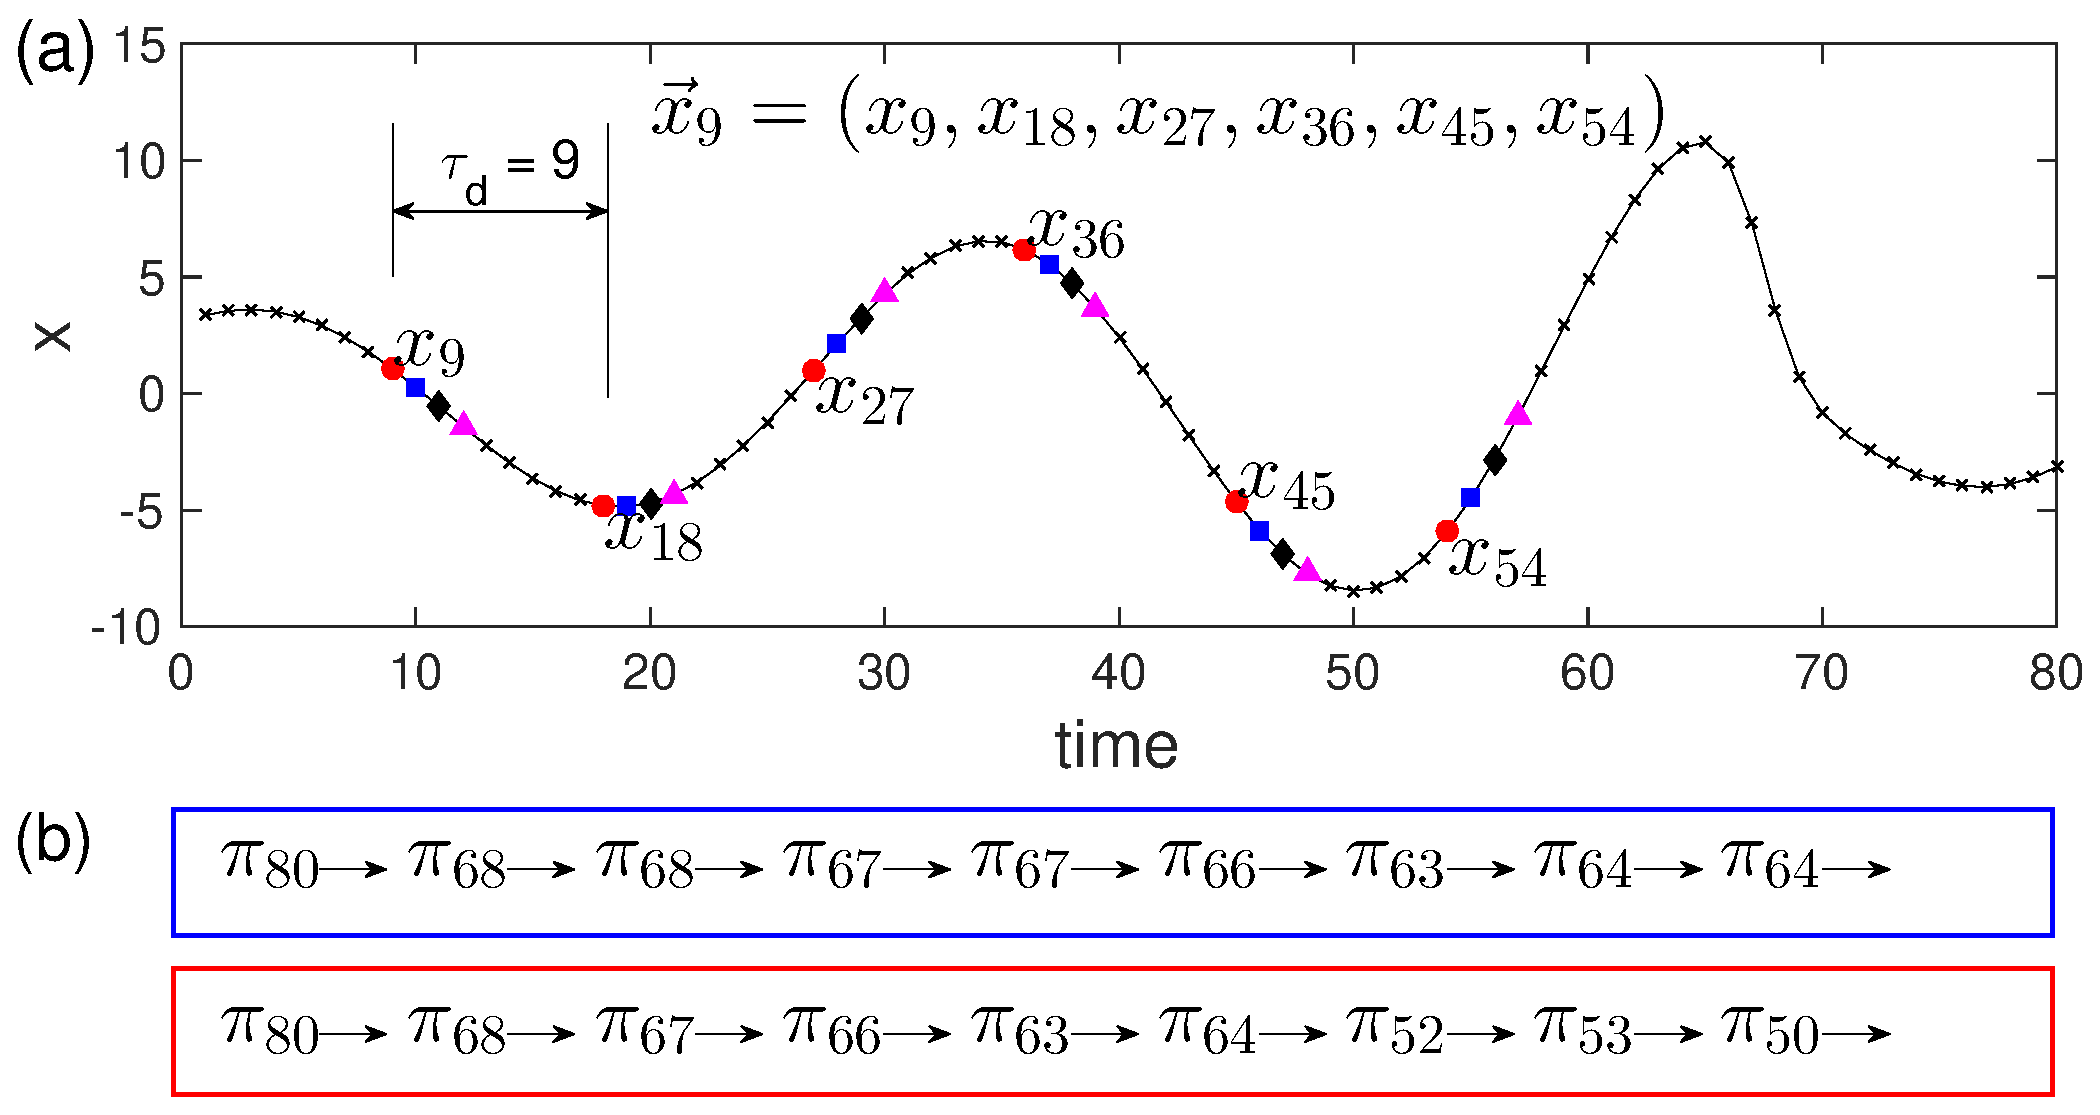
\includegraphics[width=1.3\columnwidth]{timeseriesOPexample.eps}
\caption{(Color online) Illustrative example showing ordinal pattern definitions and evolution. \textcolor{red}{Panel} (a) shows an embedding vector $\vec{x}_{9}$ with embedding parameters $\tau_d = 9$ and $D = 6$. (b) The resulting series of ordinal patterns before (top) and after (bottom) removal of all self-transitions. \label{fig:OPexample}}
\end{figure*}

Now, let us transfer the above idea from one to two series of ordinal patterns $\pi_i^{X}$ and $\pi_j^{Y}$ constructed from two possibly interacting systems $X$ and $Y$, respectively, as schematically shown in Fig.~\ref{fig:patternSeriesCond}. For $X$ exhibiting an ordinal pattern $\pi_i$ at some time $t$, we compute the time-lagged co-occurrence frequencies with all ordinal patterns of $Y$ to be observed at time $t+\tau$, i.e., $p(\pi_{j}^{Y}(\tau) | \pi_i^{X})$. When $\tau = 0$, we study the simultaneous co-occurrence of ordinal patterns in both sequences. In turn, non-zero delays $\tau$ capture possible indications of causal relationships among the two systems since it commonly takes some time for the driven process to respond properly to the driving system. An example of $p(\pi_{j}^{Y}(\tau) | \pi_i^{X})$ for two unidirectionally ($X \to Y$) coupled linear stochastic systems \cite{LiPRE2018}
\begin{equation} \label{eq:B}
A: \left \{ \begin{aligned}
x_{t+1} &= -0.3 x_{t} + \varepsilon_t, \\
y_{t+1} &= 0.3 y_{t} - 0.9 x_{t} + \eta_t,
\end{aligned}
\right.
\end{equation}
(with $\{ \varepsilon_t \}$ and $\{ \eta_t \}$ being independent and identically distributed (i.i.d.) Gaussian \textcolor{red}{white noise processes with} zero mean and unit variance) with delay $\tau = 1$ is shown in Fig.~\ref{fig:conditionTranOP}. Figure~\ref{fig:conditionTranOP}(a, b) reveals that both cases of $\tau = -1$ and $\tau = 0$ result in rather homogeneous values of $p(\pi_{j}^{Y}(\tau) | \pi_i^{X})$. By contrast, for $\tau=1$, $p(\pi_{j}^{Y}(\tau) | \pi_i^{X})$ presents markedly non-uniform co-occurrence frequencies among the $D!$ ordinal patterns of $Y$ as shown in Fig.~\ref{fig:conditionTranOP}(c). Furthermore, this heterogeneous pattern co-occurrence has been observed for all reference patterns $\pi_i^{X}$ ($i = 1, \dots, D!$) in $X$, as shown in the two-dimensional plots in Fig.~\ref{fig:conditionTranOP}(d-f). More specifically, the heterogeneous time-lagged conditional co-occurrence frequencies of $\pi_j^{Y}$ given the reference pattern $\pi_i^{X}$ for different delays $\tau$ as shown in Fig.~\ref{fig:conditionTranOP}(a-c) are respectively represented by one column in Fig.~\ref{fig:conditionTranOP}(d-f). 

\begin{figure}
	\centering
	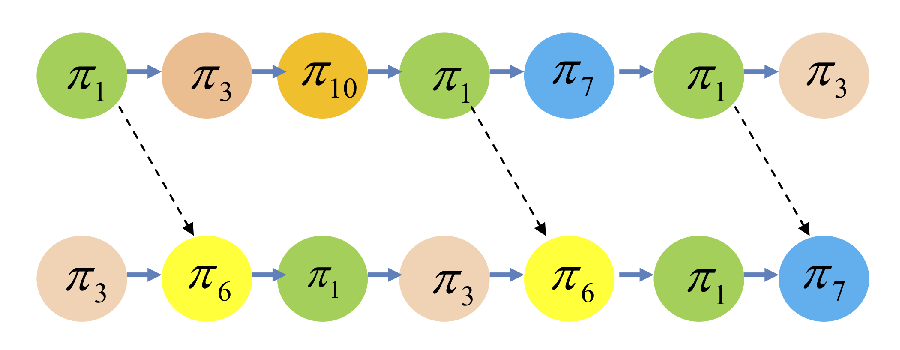
\includegraphics[width=\columnwidth]{patternSeriesCondition.eps}
\caption{(Color online) Schematic illustration of the OPTN analysis for two series of ordinal patterns with a unidirectional coupling $X \to Y$ with a coupling delay of $1$. The time-lagged conditional co-occurrences of the patterns $\pi_i^{X}$ and $\pi_{j}^{Y}(\tau)$ are indicated by dashed arrows. In this example, we observe two cases of occurrences of $\pi_6$ in the $Y$ series when $X$ presents the pattern $\pi_1$ at the previous time step.  \label{fig:patternSeriesCond}}
\end{figure}

\begin{figure*}
	\centering
 	\includegraphics[width=2\columnwidth]{cond_allPatterns.eps}
\caption{(Color online) Graph representation of time-lagged conditional co-occurrence frequencies for the ordinal patterns $\pi_{j}(\tau)$ of the $Y$ series when $X$ has the same randomly chosen ordinal pattern $\pi_i^{X}$ for $D = 5$. \textcolor{red}{(a-c)} The pattern $\pi_i^{X}$ is \textcolor{red}{considered fixed and} placed in the center while the different patterns $\pi_{j}^{Y}$ are \textcolor{red}{varied and} aligned on the unit circle. The thickness of each connecting line corresponds to the time-lagged occurrence frequency of $\pi_j^{Y}$ under the condition that $X$ has pattern $\pi_i^{X}$. \textcolor{red}{Panels} (a-c) are for one reference ordinal pattern $\pi_i^{X}$ \textcolor{red}{with} (a) $p(\pi_{j}^{Y}(\tau=-1) | \pi_{i}^{X}) $, (b) $p(\pi_j^{Y}(\tau=0) | \pi_i^{X})$, and (c) $p(\pi_{j}^{Y}(\tau=1) | \pi_i^{X})$. Panels (d-f) give the corresponding two-dimensional plots for all patterns of $\pi_i^{Y}$ under the condition that $X$ has reference pattern $\pi_i^{X}, i = 1, \dots, D!$. Note that the missing patterns have been indicated by white dots, which are frequently found in the case of $\tau = 1$. The color bar represents the co-occurrence frequencies between patterns. 
\label{fig:conditionTranOP}}
\end{figure*}

From the described construction of OPTNs for the case of two time series, it is obvious that the resulting networks exhibit two distinct types of nodes, corresponding to the ordinal patterns $\pi_i^X$ of $X$ and $\pi_j^Y$ of $Y$, respectively, and exclusively (weighted and directed) links from any $\pi_i^X$ to any $\pi_j^Y$ based on the corresponding conditional co-occurrence frequencies. Hence, this type of network constitutes a weighted and directed bipartite network. Given that specific network properties tailored to describing the topological characteristics of such networks are rather limited as \textcolor{red}{compared} to unweighted, undirected, and unipartite graphs, in what follows we will introduce a suite of network characteristics that are specifically designed to capture different aspects of the underlying heterogeneity of link weights.

\section{Complexity measures for bipartite OPTNs} \label{sec:measures}

Based on our qualitative observations as shown in Fig.~\ref{fig:conditionTranOP}, in the following we propose a suite of measures to quantitatively characterize the heterogeneous co-occurrence of ordinal patterns in two time series. All these measures will make use of the time-lagged co-occurrence frequencies between ordinal patterns in the two time series under study.

\textcolor{red}{\subsection{Standard deviation of conditional co-occurrence frequencies}}
First, we note that for one reference pattern $\pi_i^{X}$ of $X$, the heterogeneity of the \emph{conditional} frequencies of patterns $\pi_{j}^{Y}$ in $Y$ at a time lag $\tau$ can be simply characterized by their corresponding standard deviation
\begin{equation}
\sigma_i^{X} (\tau) = \sqrt{\frac{\sum_{j = 1}^{D!} [p(\pi_{j}^{Y}(\tau) | \pi_i^{X}) - \overline{p(\pi_{j}^{Y}(\tau) | \pi_i^{X})}]^{2} }{D!}}, 
\label{eq:sigmaX}
\end{equation}
where $\overline{\bullet}$ denotes here the average over all patterns $\pi_{j}^{Y}$ in $Y$, i.e., $\overline{p(\pi_{j}^{Y}(\tau) | \pi_i^{X})}$ gives the mean probability of all patterns $\pi_{j}^{Y}(\tau)$ in the series $Y$ to occur at a time-lag $\tau$ under the condition that the series $X$ has exhibited the pattern $\pi_i^{X}$. In the case of no interdependency between $X$ and $Y$, $p(\pi_{j}^{Y}(\tau) | \pi_i^{X})$ will be independent of $\pi_i^{X}$ and, hence, solely reflect the marginal distribution of the ordinal patterns $\pi_j^{Y}$, so that $\overline{p(\pi_{j}^{Y}(\tau) | \pi_i^{X})}=1/D!$ because of the normalization of probabilities. In such a case, any non-zero value of $\sigma_i^{X}$ simply originates from the heterogeneity of the frequency distribution of ordinal patterns in $Y$. If this distribution is homogeneous, the numerator of Eq.~\eqref{eq:sigmaX} will be (close to) zero. In turn, if there is dependency between $Y$ and $X$, $\overline{p(\pi_{j}^{Y}(\tau) | \pi_i^{X})}\neq 1/D!$ and, hence, $\sigma_i^{X}(\tau)$ will differ from the aforementioned benchmark (independence) case. Hence, any significant deviation of $\sigma_i^{X}(\tau)$ from this benchmark, which can be computed by replacing in Eq.~\eqref{eq:sigmaX} $\overline{p(\pi_{j}^{Y}(\tau) | \pi_i^{X})}$ by $\pi_j^{Y}$, will indicate the presence of (time-lagged) coupling between both systems in the (causal) sense of $X$ determining the behavior of $Y$.

While the above considerations have focused on a single ordinal pattern $\pi_i^{X}$ in $X$ only, we obtain a general measure for the corresponding dependency between $X$ and $Y$ by summing up the values found for all ordinal patterns $\pi_i^{X}$ as
\begin{equation}
\sigma_{X\to Y} (\tau) = \sum_{i=1}^{D!} \sigma_{i}^{X} (\tau). 
\end{equation}

\textcolor{red}{\subsection{Shannon entropy of conditional co-occurrence frequencies}}
Our second characteristic property is based on a similar rationale as a measure recently proposed in ref.~\cite{McCullough2017b}. Here, we first \textcolor{red}{characterize the heterogeneity of per-node} ordinal pattern co-occurrence by the Shannon entropy
\begin{equation} \label{eq:localH}
H_{X \to Y}^{\pi_i}(\tau) = - \sum_{j=1}^{D!} p(\pi_{j}^{Y}(\tau) | \pi_i^{X}) \log_2 p(\pi_{j}^{Y}(\tau) | \pi_i^{X}), 
\end{equation}
where the summation runs over all possible patterns of $\pi_j^{Y}(\tau)$. Note that for each pattern $\pi_i^{X}$ and delay $\tau$, a normalization is introduced by $\sum_{j=1}^{D!} p(\pi_{j}^{Y}(\tau) | \pi_i^{X}) = 1$. Since patterns $\pi_i$ can have different empirical frequencies $p(\pi_i^{X})$, we further compute the expectation value of the co-occurrence entropy of the whole bipartite OPTN as 
\begin{equation}  \label{eq:globalH}
H_{X \to Y}(\tau) = \sum_{i=1}^{D!} p(\pi_i^{X}) H_{X \to Y}^{\pi_i}(\tau), 
\end{equation}
which we call global ordinal pattern co-occurrence entropy. 

For a memoryless and stationary stochastic process, we may expect $p(\pi_i^{X} )= \frac{1}{D!}$ for any pattern order $D$. Accordingly, the local (per-node) co-occurrence entropy of Eq.~\eqref{eq:localH} simplifies as 
\begin{equation}
p(\pi_{j}^{Y}(\tau) | \pi_i^{X}) \log_2 p(\pi_{j}^{Y}(\tau) | \pi_i^{X}) = \frac{1}{D!} \log_2 \frac{1}{D!}. 
\end{equation}
Therefore, the global co-occurrence entropy (Eq.~\eqref{eq:globalH}) has a maximal value $H_{X \to Y} = \log_2 D!$ if all $D!$ patterns are distributed uniformly in both, $X$ and $Y$. For example, ${\color{red}H_{X \to Y}^{\text{max}}} \approx 6.9$ when $D = 6$ for two series of ordinal patterns that are obtained from two i.i.d. noise processes. We note that this observation might be used for obtaining a proper re-normalization of $H_{X \to Y}(\tau)$, which shall however not \textcolor{red}{be} further pursued here.

\textcolor{red}{\subsection{Kullback-Leibler divergence of conditional co-occurrence frequencies}}
Finally, we propose a third measure to capture possible causal influences of $X$ on $Y$, which quantifies how much more heterogeneous the co-occurrence frequencies $p(\pi_{j}^{Y} | \pi_i^{X})$ are in comparison with the marginal distribution $p(\pi_j^{Y})$ (without prior knowledge of the driving process). For this purpose, we compute the node-wise Kullback-Leibler divergence (KLD) in the following way: 
\begin{equation} \label{eq:localKLD}
\text{KLD}^{\pi_i}(\tau) = \sum_{j=1}^{D!} p(\pi_{j}^{Y}(\tau) | \pi_i^{X}) \log_2 \frac{p(\pi_{j}^{Y}(\tau) | \pi_i^{X})}{p(\pi_j^{Y})}, 
\end{equation}
which appears to be closer to the Granger-type idea of causality than the two previous measures. Here, we use the KLD to distinguish between two probability distributions $p(\pi_{j}^{Y} | \pi_i^{X})$ and $p(\pi_j^{Y})$, the value of which vanishes if and only if the ordinal pattern series $\{\pi_i^{X}\}$ and $\{\pi_j^{Y}\}$ are independent, while any positive value suggests a possible directed influence from $X$ to $Y$. As a corresponding global characteristic, the expected KLD of the whole network is calculated as
\begin{equation}  \label{eq:globalKLD} 
\text{KLD}_{X \to Y}(\tau) = \sum_{i=1}^{D!} p(\pi_i^{X}) \text{KLD}^{\pi_i}(\tau), \
\end{equation}
where the summation runs over all patterns $\pi_i^{X}$ of $X$. 

\textcolor{red}{\subsection{Relationship with existing measures}}

\textcolor{red}{The three statistical characteristics of co-occurrence frequencies introduced above should be seen as representatives of a larger class of nonlinear measures based on symbolic sequences of ordinal patterns, some of which have already been used in the existing literature. In this spirit, we may emphasize that entropic characteristics like $H_{X\to Y}(\tau)$ and KLD are based on the same rationale as other information-theoretic measures like conditional mutual information or transfer entropy. These as well as closely related measures have been originally defined for general symbolic sequences and, hence, can also be applied to sequences of ordinal patterns.}

\textcolor{red}{Two notable conceptually related characteristics previously used for similar purposes of detecting directional coupling among time series include the permutation conditonal mutual information (PCMI)~\cite{LiNI2010} and (symbolic) transfer entropy ((S)TE)~\cite{schreiber_prl2000,Staniek2008}. Although both exhibit certain similarities with our co-occurrence entropy and KLD, they differ in important details. The PCMI $I_{X\to Y}(\tau)$ can be written as the conditional mutual information between the symbols $\pi^Y(\tau)$ and $\pi^X$ given $\pi^Y$. A similar idea applies to the (S)TE; in fact, the simplest version of (S)TE taking only one past time step into account would be fully equivalent to the PCMI. Both (S)TE and PCMI are thus based on the idea of predictive (Granger) causality, i.e., to use knowledge about the past of both processes to predict the future of one of them.}

\textcolor{red}{More specifically, the time-delayed conditional mutual information underlying PCMI quantifies the interaction information from $X$ to $Y$ by the difference between $p(\pi_j^{Y}(\tau); \pi_k^{Y} | \pi_i^{X})$  and $p(\pi_j^{Y}(\tau); \pi_k^{Y})$. Similarly, S(TE) characterizes the coupling between two series by the amount of uncertainty reduced in the prediction of future values of $\pi^{Y}(\tau)$ (knowing the past values of $\pi^{Y}$) due to the knowledge of $\pi^{X}$ as the possible causal effect. Accordingly, the information transfer from $X$ to $Y$ is expressed in terms of the dissimilarity between the two probabilities $p(\pi_j^{Y}(\tau) | \pi_k^{Y}, \pi_i^{X})$  and $p(\pi_j^{Y}(\tau) | \pi_k^{Y})$.}

\textcolor{red}{Other than PCMI and (S)TE, $H_{X\to Y}$ is defined as the weighted-average permutation entropy of $Y$ under the respective condition of the previous occurrence of each possible symbol $\pi_i^X$ in $X$, where the weights are given by the probabilities of $\pi_i^X$. In other words, both $H_{X\to Y}$ and also KLD do not involve any conditioning on the permutation $\pi_j^Y$ observed at the current point in time, but just take the past symbol in one series to statistically evaluate the next one in the other series. That is, our three measures provide estimates for the coupling strength between two time series at a given time lag, which can be used to infer causality in the sense of a cause preceding the effect, but not in the predictive sense of causality as PCMI and (S)TE.}

\textcolor{red}{Further differences between the different measures exist regarding the choice of the parameter $\tau$. In PCMI~\cite{LiNI2010}, $\tau$ has been suggested not to be smaller than the embedding dimension $D$. In turn, in STE~\cite{Staniek2008} $\tau$ is treated as an algorithmic parameter which is commonly taken as $\tau = 1$, which is considered to be always applicable as long as a meaningful natural sampling rate of the time series is given. According to our discussions presented in the previous subsections, our measures interpret $\tau$ in a somewhat different way, i.e., as a continuous parameter that has to be systematically varied in order to identify the correct coupling delay, thereby treating $\tau$ explicitly as an unknown variable.}


\section{Numerical examples} \label{sec:res}
In \textcolor{red}{the following} section, we demonstrate that the time-lagged ordinal pattern co-occurrence complexity measures introduced in section~\textcolor{red}{\ref{sec:measures}} can capture causal interactions in both, unidirectional and bidirectional coupling configurations. In order to illustrate this, we consider examples from two typical classes of time-discrete dynamical systems: simple stochastic processes and chaotic maps. 

\subsection{Coupled stochastic processes} \label{sec:GCs}
We first test our measures regarding their capability to correctly identify coupling directions and delays among simple one-dimensional stochastic processes. For this purpose, we study two examples in a unidirectional coupling configuration and two others in a bidirectional setting. Moreover, we consider cases with a single delay term versus such with more than one delay, as well as nonlinear model versions obtained by static nonlinear transformations of the first subsystem as proposed in ref.~\cite{LiPRE2018}.

In all considered models, we generate time series $\{ x_t \}$ and $\{ y_t \}$ of length $N=10^{5}$, which are then used to construct ordinal pattern representations with the embedding parameters $D = 5$ and $\tau_d = 100$. We have checked that our results do not change qualitatively if other parameter combinations are chosen (not shown). The relevance of all inferred interaction delays has been confirmed by switching the roles of $X$ and $Y$ (for instance, a positive delay $\tau$ from $X$ to $Y$ should coincide with a negative delay $-\tau$ when exchanging the two systems). 

The results presented in the following are based on averages over 20 independent realizations of the considered processes. {\color{red}We emphasize that the differences between the individual realizations are in general very small. Hence, in the following figures we will omit error bars indicating the corresponding ensemble standard deviations, since they appear negligible in comparison with the overall found values of all considered OPTN based complexity measures.}

\subsubsection{Unidirectional coupling}

We start with the system of two coupled linear stochastic systems from Eq.~\eqref{eq:B}. A nonlinear transformation $f(x) = \left[\frac{x + | x |}{2}\right]^{5}$ is applied to each realization of the first system $X$, and the resulting realization of the transformed system $\tilde{X}$ is denoted as $\{\tilde{x}_t\}$. 

Based on the resulting sequences of ordinal patterns, we compute the three measures $\sigma_{X \to Y}(\tau)$, $H_{X \to Y}(\tau)$ and $\text{KLD}(\tau)$ and show the corresponding results in Fig.~\ref{fig:stdHeqB}. We clearly find at $\tau = 1$ a unique maximum of $\sigma_{X \to Y}(\tau)$ and $\text{KLD}(\tau)$ (Fig.~\ref{fig:stdHeqB}(a,e)) while $H_{X\to Y}(\tau)$ presents a minimum (Fig.~\ref{fig:stdHeqB}(c)). Thus, all three measures consistently suggest that there is an interaction from $X$ to $Y$ at a delay $\tau = 1$. Almost identical results are obtained if the system $X$ is replaced by its nonlinearly transformed counterpart $\tilde{X}$ (Fig.~\ref{fig:stdHeqB}(b,d,f)). 

\begin{figure}
	\centering
	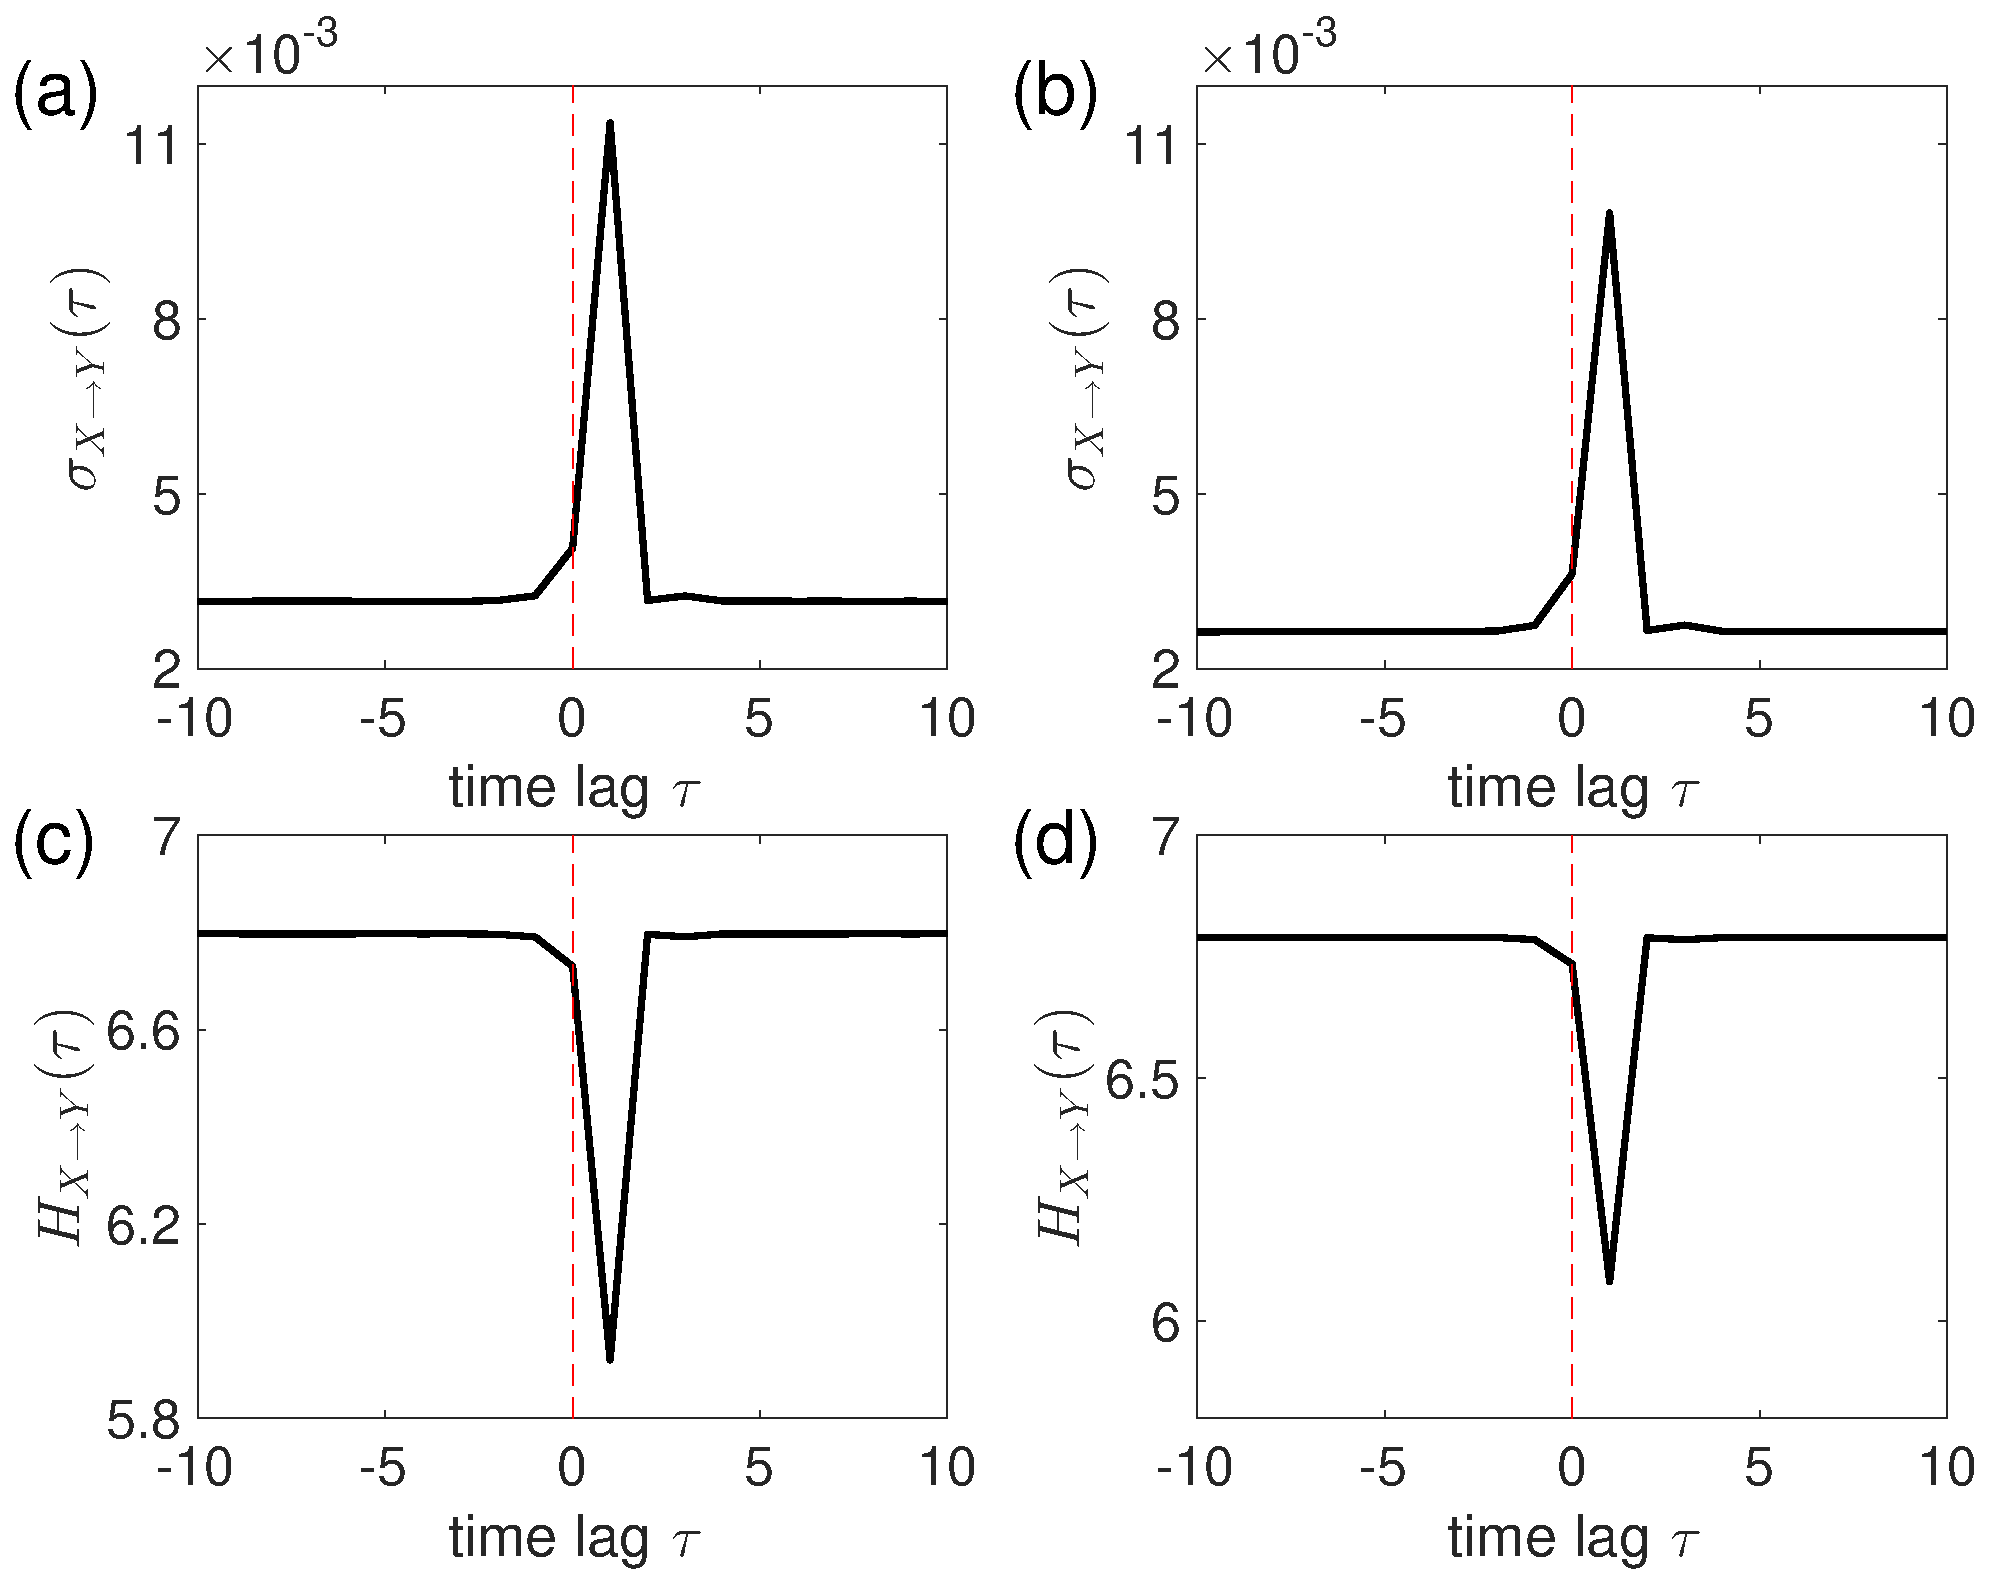
\includegraphics[width=\columnwidth]{E_B.eps}
	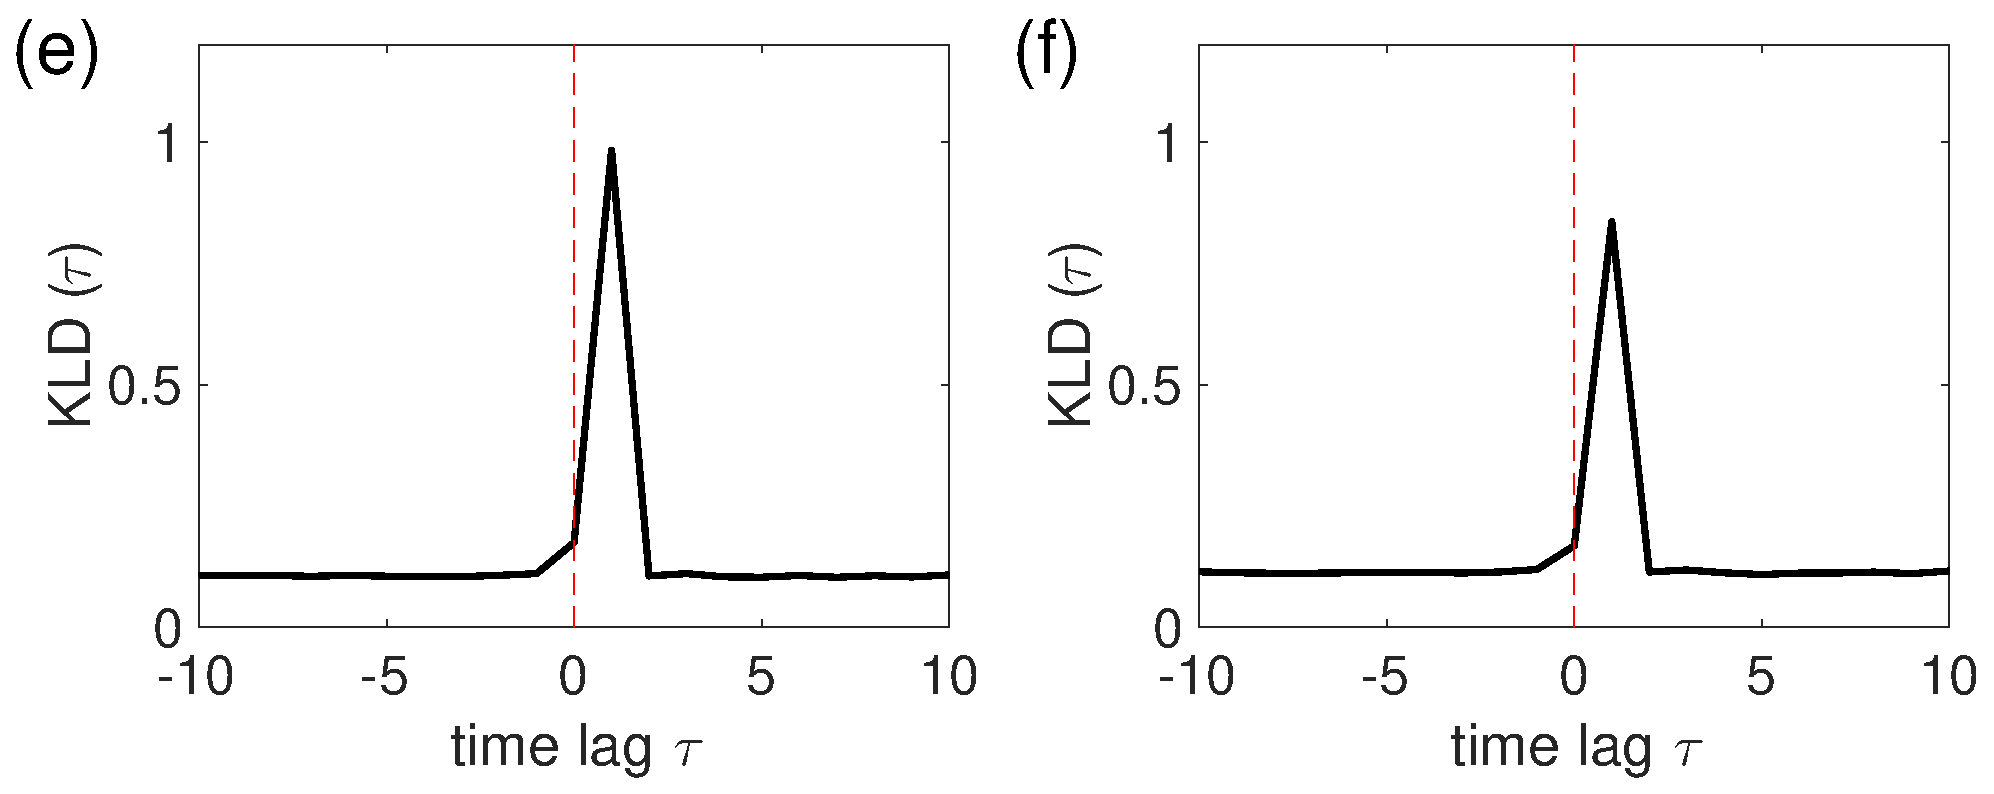
\includegraphics[width=\columnwidth]{KL_B.eps}
\caption{(Color online) Values of three ordinal pattern co-occurrence complexity measures in dependence on the mutual delay $\tau$ for realizations of Eq.~\eqref{eq:B}: (a,b) $\sigma_{X\to Y}(\tau)$, (c,d) $H_{X \to Y}(\tau)$, (e,f) $\text{KLD}(\tau)$. \textcolor{red}{Panels} (a,c,e) show the results for realizations from the linear model, while (b,d,f) correspond to the nonlinear transformation of the first subsystem as described in the text. The vertical red dashed lines indicate the values for vanishing mutual delay ($\tau=0$).
\label{fig:stdHeqB}}
\end{figure}

When introducing more interaction delays from $X$ to $Y$, $\sigma_{X\to Y}(\tau)$, $H_{X \to Y}(\tau)$ and $\text{KLD}(\tau)$ exhibit additional maxima and minima, respectively, at various values of $\tau$. To illustrate this, we generate time series from the following linear system~\cite{LiPRE2018}:
\begin{equation} \label{eq:C}
B: \left \{ \begin{aligned}
x_{t+1} &= - \sum_{k=0}^{7} c_k x_{t-k} + \varepsilon_t, \\
y_{t+1} &= - \sum_{k=0}^{7} c_k y_{t-k} + 100 \sum_{k=0}^{8} c_k x_{t-k} + \eta_t,
\end{aligned}
\right.
\end{equation}
where $\varepsilon_t$ and $\eta_t$ are again independent Gaussian random variables. In this model, there are nine interaction terms from $X$ to $Y$ at different delays. By taking the coefficients $\{ c_k \}$ from the polynomial $\sum_{k=0}^{8} c_k z^{k} = [(1 - r e^{-2\pi i f}z)(1 - r e^{2\pi i f} z)]^{4}$ with $f = 0.1$ and $r = 0.8$ \textcolor{red}{as studied in ref.}~\cite{LiPRE2018}, it is ensured that the evolution of $Y$ is influenced more by the interaction terms at smaller delays than those with larger delays. A nonlinearly transformed signal $\tilde{X}$ is obtained by setting $\tilde{x}_{t} = x_{t}^{5}$. 

In comparison with the previous case of a system with only one interaction delay $\tau$ (Fig.~\ref{fig:stdHeqB}), the presence of multiple interaction delays is clearly identified by all three measures (Fig.~\ref{fig:stdHeqC}). However, since these interactions occur at subsequent delays, the corresponding effects partially cancel each other, resulting in a succession of local maxima and minima of these measures. Hence, not all individual delays are identified by our approach in the considered setting. Notably, the nonlinearly transformed version of the model shows again results that are almost equivalent to those of the underlying linear version.

\begin{figure}
	\centering
	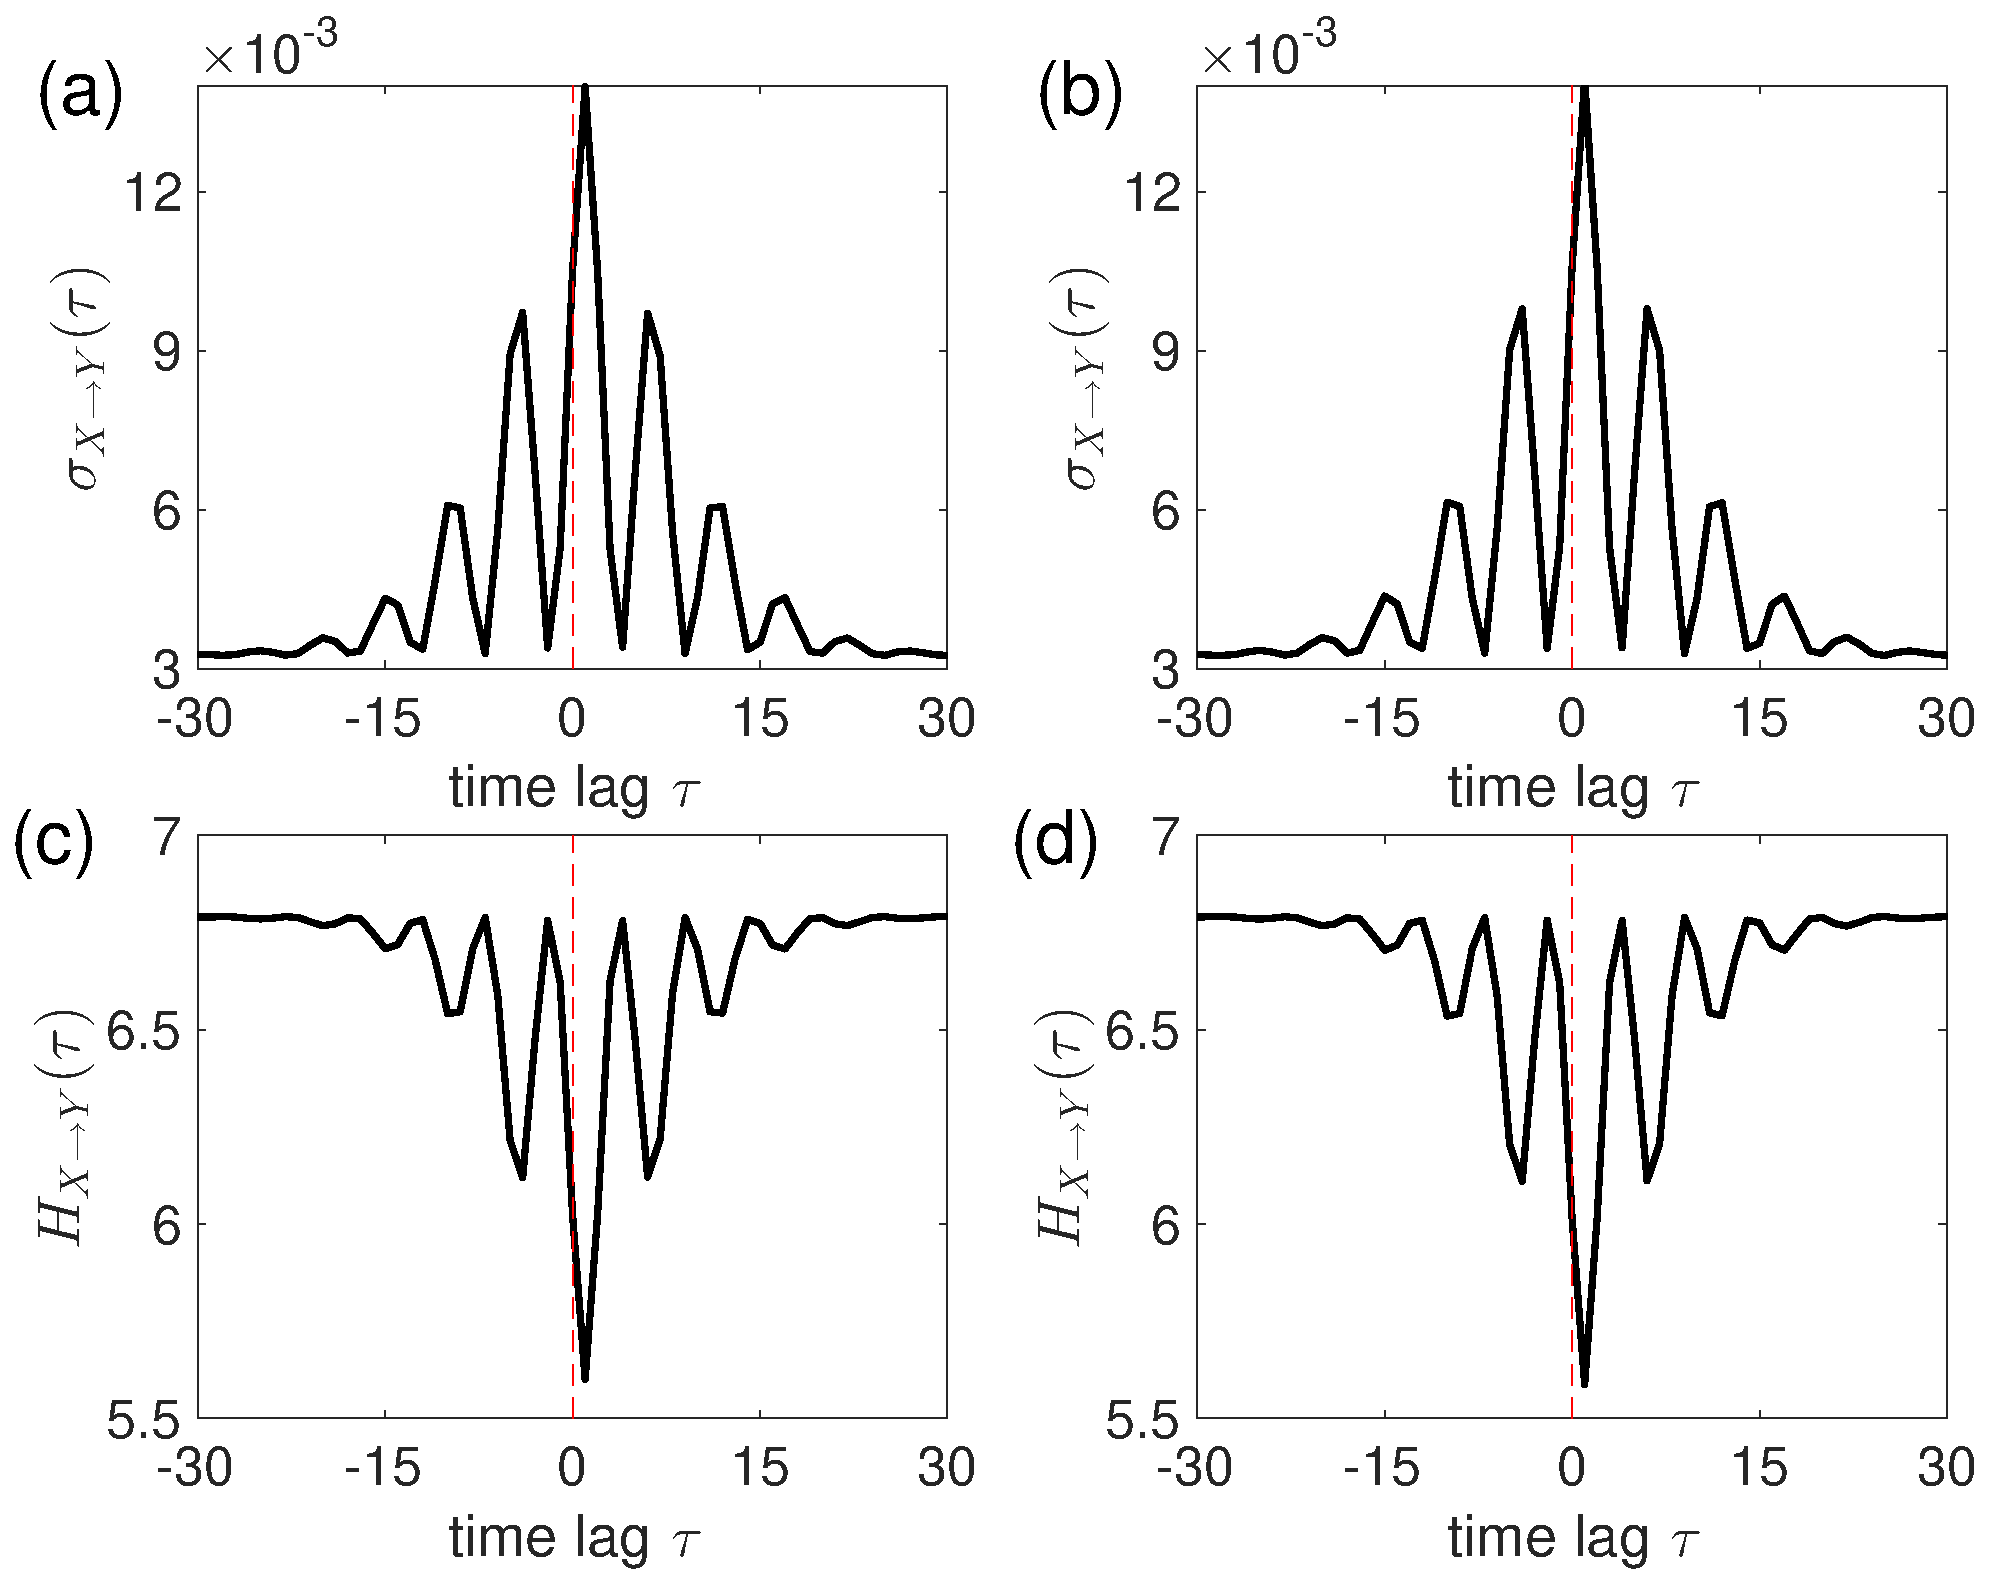
\includegraphics[width=\columnwidth]{E_C.eps}
	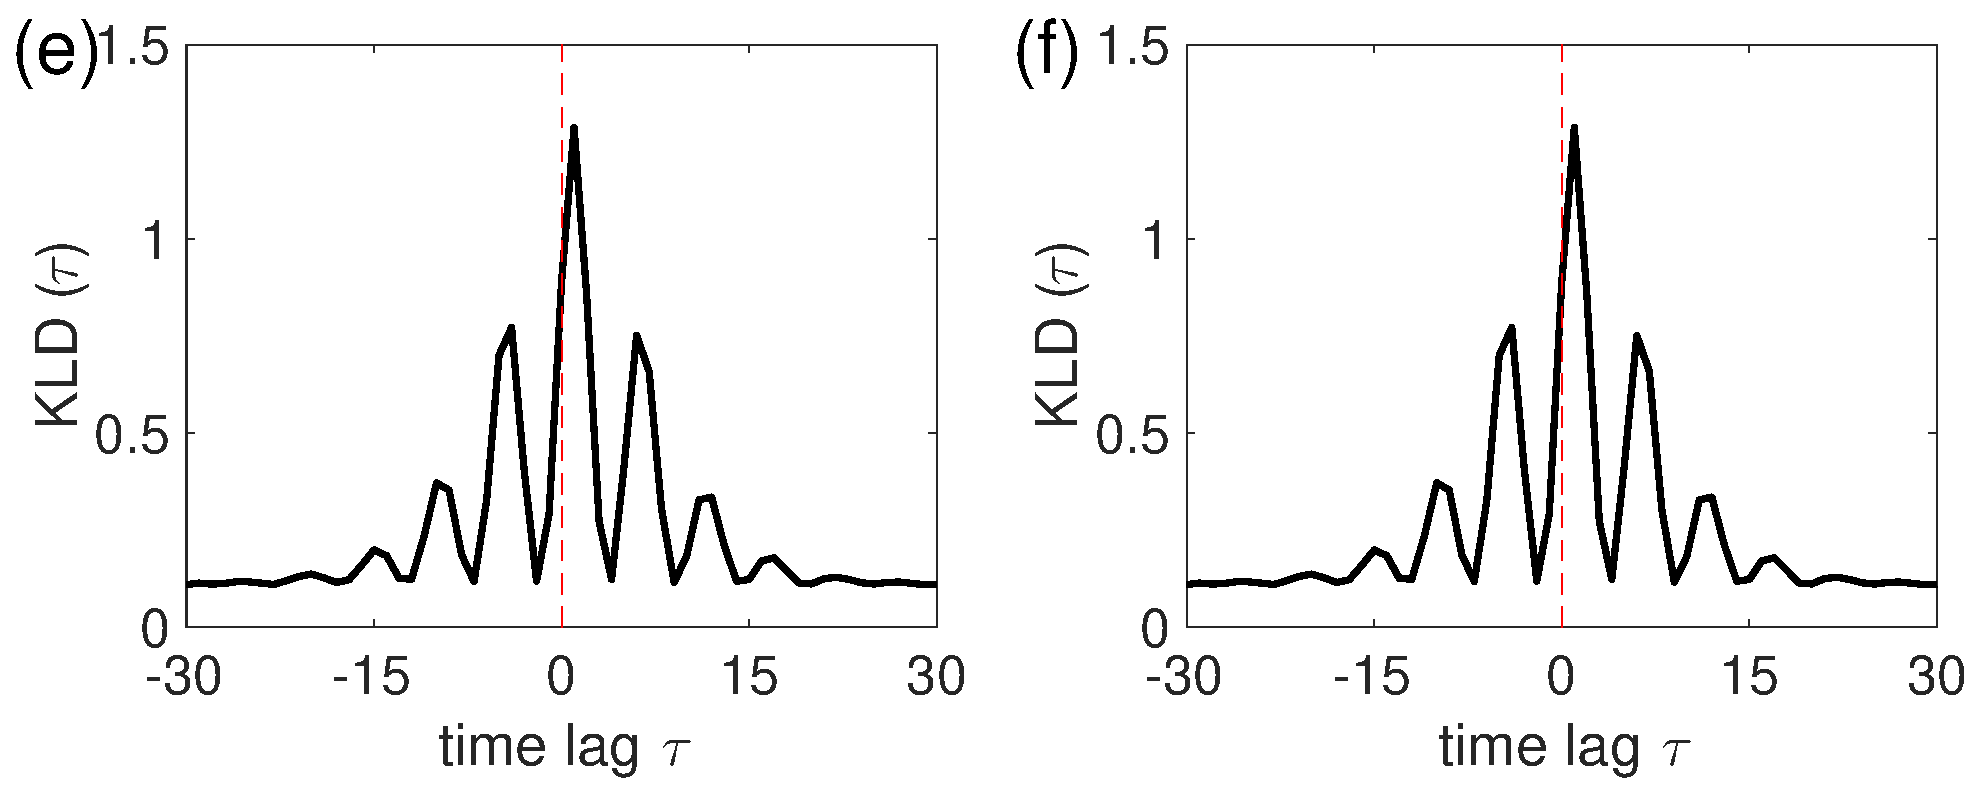
\includegraphics[width=\columnwidth]{KL_C.eps}
\caption{(Color online) Same as in Fig.~\ref{fig:stdHeqB} but for Eq.~\eqref{eq:C}.  \label{fig:stdHeqC}}
\end{figure}

\subsubsection{Bidirectional coupling}

Next, we consider a symmetric bidirectional interaction with a delay of $\tau = 1$ from $X$ to $Y$ and from $Y$ to $X$. The corresponding numerical model reads as follows: 
\begin{equation} \label{eq:D}
C: \left \{ \begin{aligned}
x_{t+1} &= - 0.5 y_{t} + \varepsilon_t, \\
y_{t+1} &= - 0.5 x_{t} + \eta_t, 
\end{aligned}
\right.
\end{equation}
where $\{ \varepsilon_t \}$ and $\{ \eta_t \}$ are again i.i.d standard Gaussian random variables. The nonlinearly transformed signal $\tilde{X}$ is obtained by \textcolor{red}{setting} $\tilde{x}_{t} = x_{t}^{2}$. In this case, $X$ influences $Y$ at a delay $\tau = 1$ while $Y$ influences $X$ at the same delay. As shown in Fig.~\ref{fig:stdHeqD}(a,c,e), both delays are correctly identified by $\sigma_{X \to Y}(\tau)$, $H_{X \to Y}(\tau)$ and $\text{KLD}(\tau)$. For the nonlinearly transformed case, this result is essentially reproduced. In all cases, the corresponding measures exhibit two large peaks/troughs at the positive time lag $\tau = 1$ and the negative time delay $\tau = -1 $. This indicates that the employed coupling is bidirectional and symmetric in both the linear and nonlinear systems. 

\begin{figure}
	\centering
	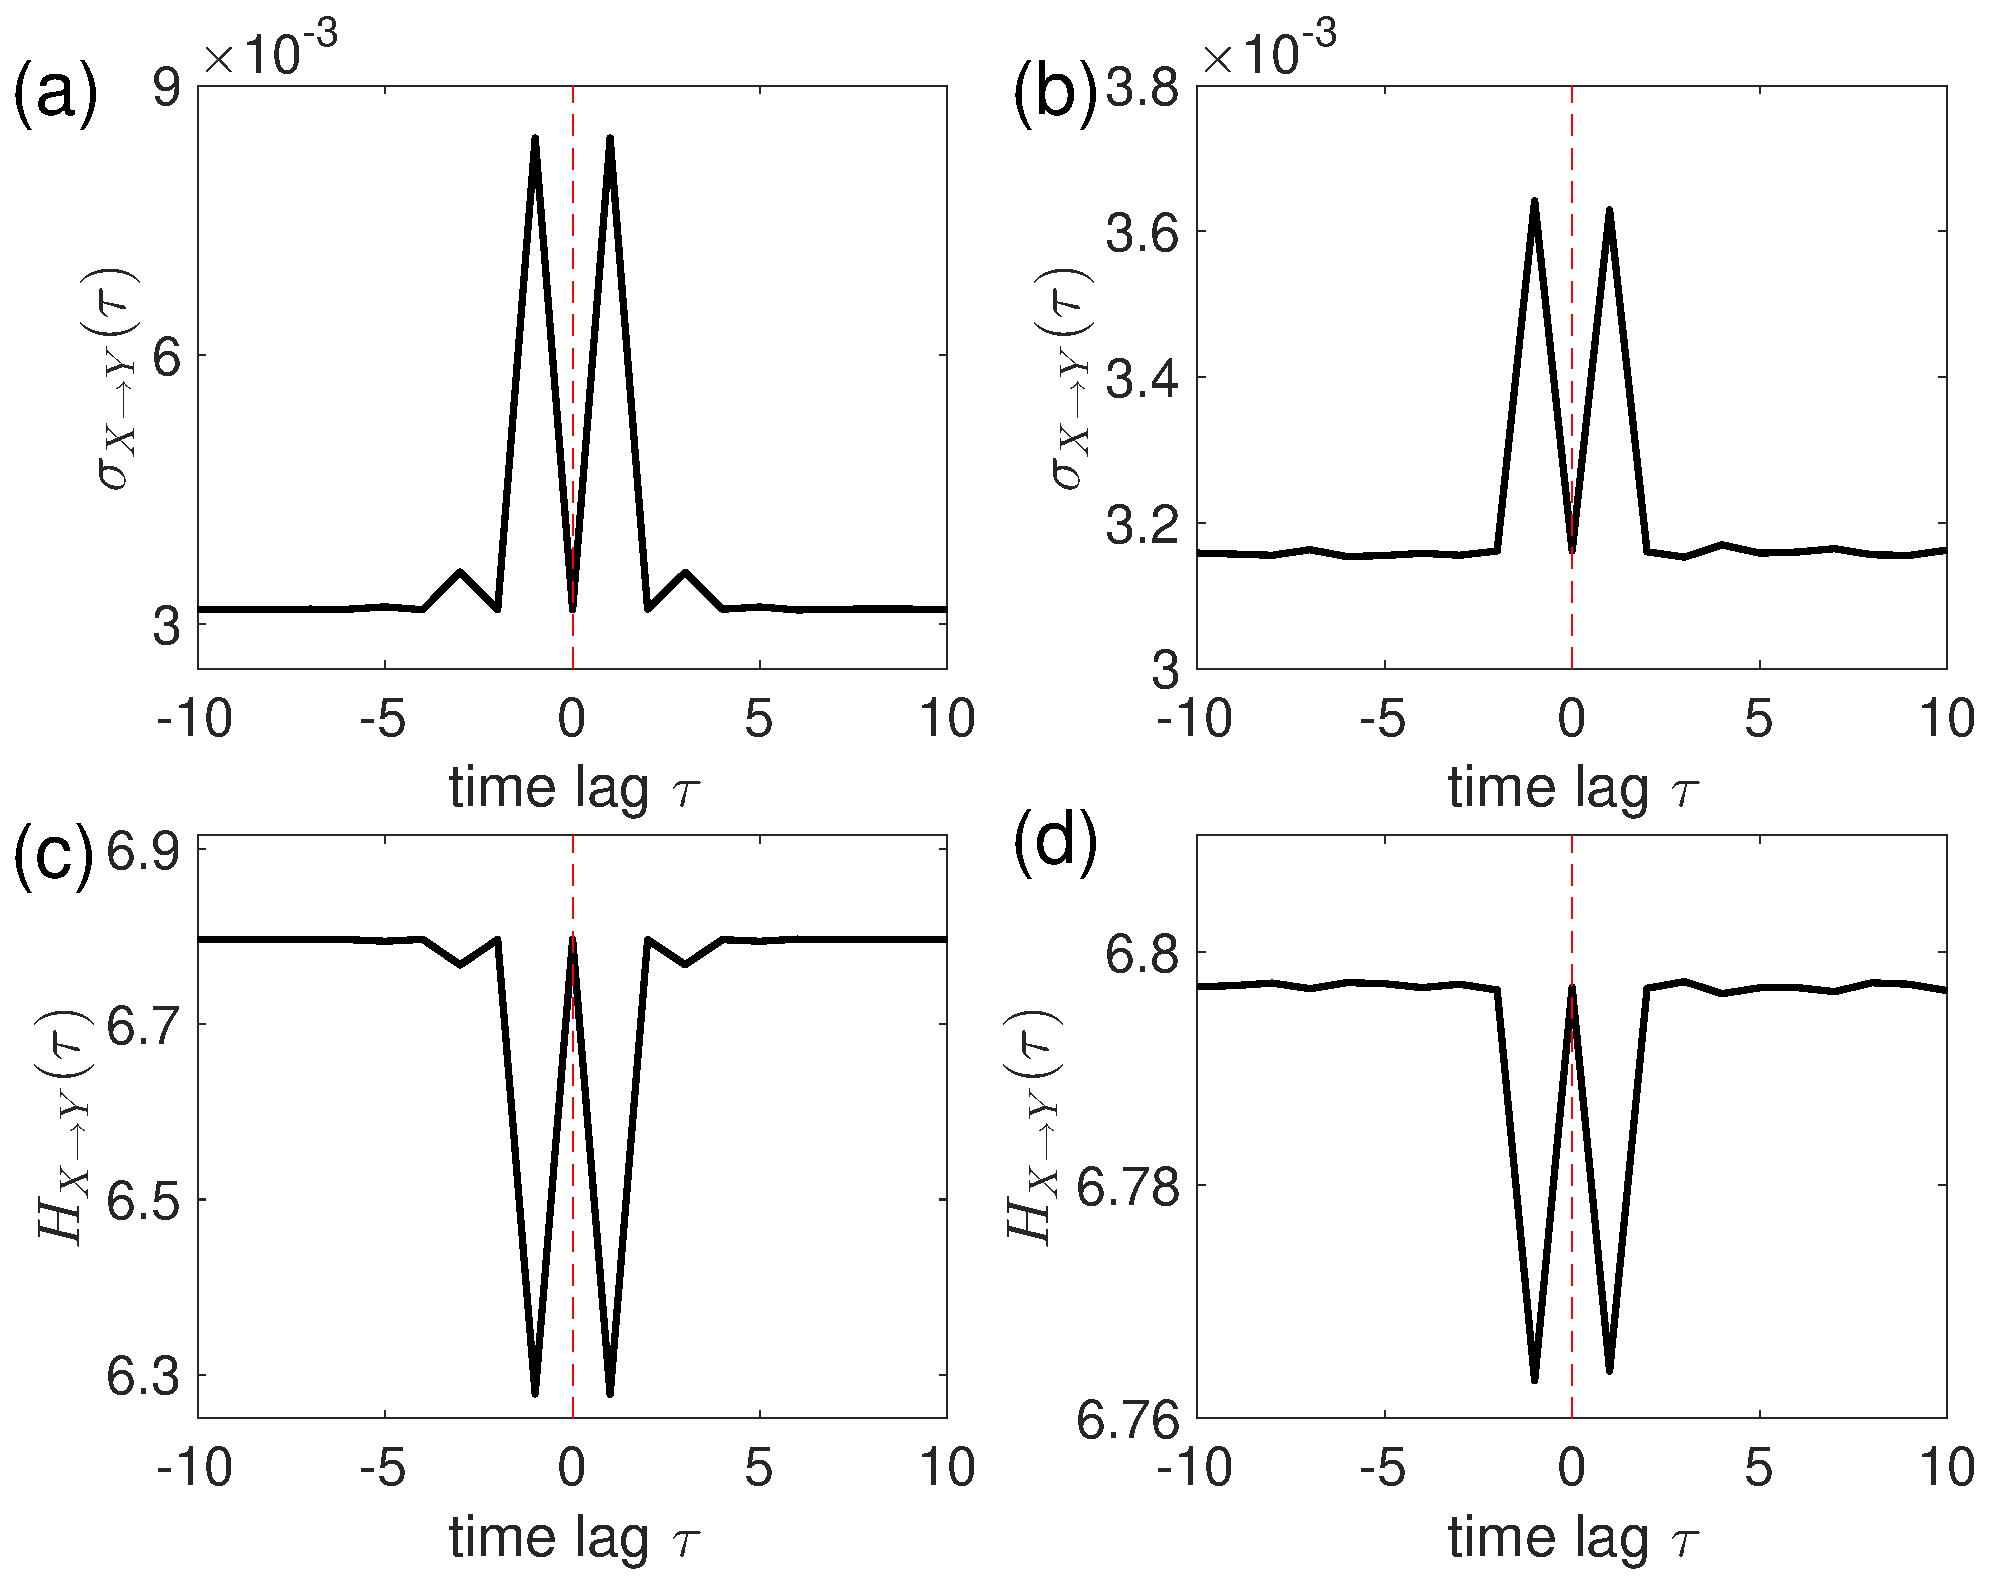
\includegraphics[width=\columnwidth]{E_D.eps}
	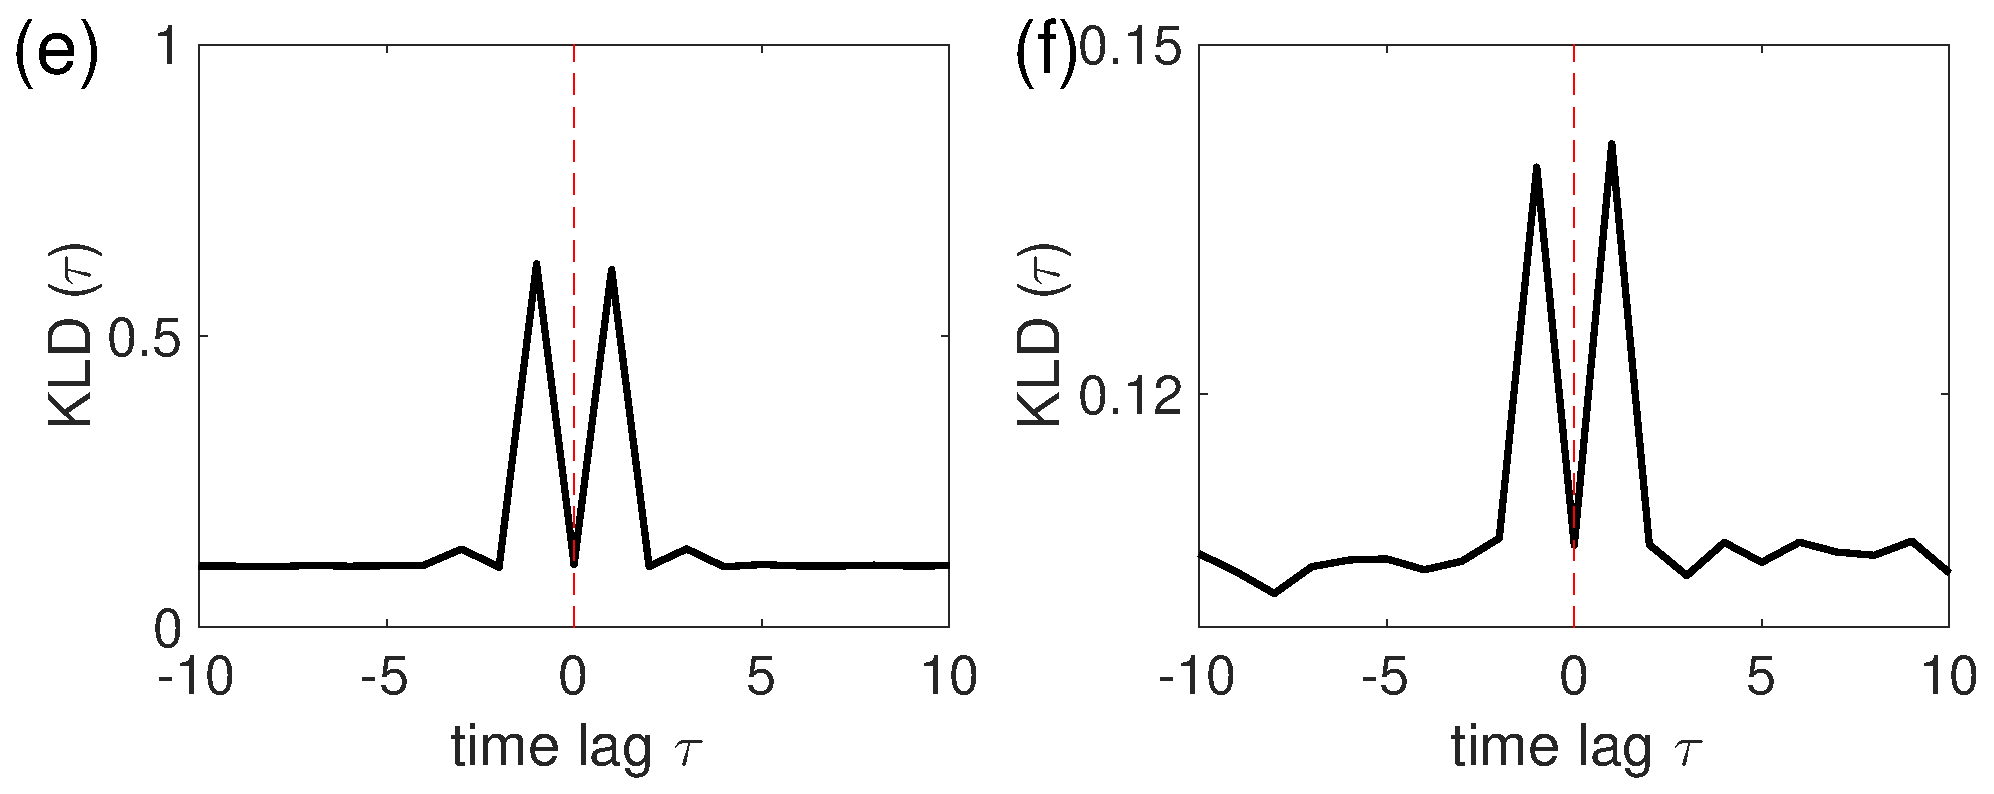
\includegraphics[width=\columnwidth]{KL_D.eps}
\caption{(Color online) Same as in Fig.~\ref{fig:stdHeqB} but for Eq.~\eqref{eq:D}.   \label{fig:stdHeqD}}
\end{figure}

As a final example of coupled stochastic processes, we consider a more challenging case of asymmetric bidirectional interactions between $X$ and $Y$. More specifically, $X$ influences $Y$ at a delay $\tau = 2$ while the interaction from $Y$ to $X$ appears at a delay $\tau = 1$. The corresponding linear stochastic model reads as follows: 
\begin{equation} \label{eq:E}
D: \left \{ \begin{aligned}
x_{t+1} &= 0.3 y_{t} + \varepsilon_t, \\
y_{t+1} &= 0.5 x_{t-1} + \eta_t, 
\end{aligned}
\right.
\end{equation}
where $\{ \epsilon_t \}$ and $\{ \eta_t \}$ are again realizations of i.i.d. Gaussian noise. The nonlinearly transformed $\tilde{X}$ is defined as $\tilde{x}_{t} = \tanh{10 x_t}$. As in the previous three examples, in both the linear and nonlinear cases, the curves of $\sigma_{X \to Y}(\tau)$, $H_{X\to Y}(\tau)$ and $\text{KLD}(\tau)$ correctly identify two delays at $\tau = -1$ and $\tau = 2$ as shown in Fig.~\ref{fig:stdHeqE}. This correctly suggests that $X (\tilde{X})$ affects $Y$ at a delay of $\tau = 2$ while $Y$ influences $X$ ($\tilde{X}$) at $\tau = 1$. 

\begin{figure}
	\centering
	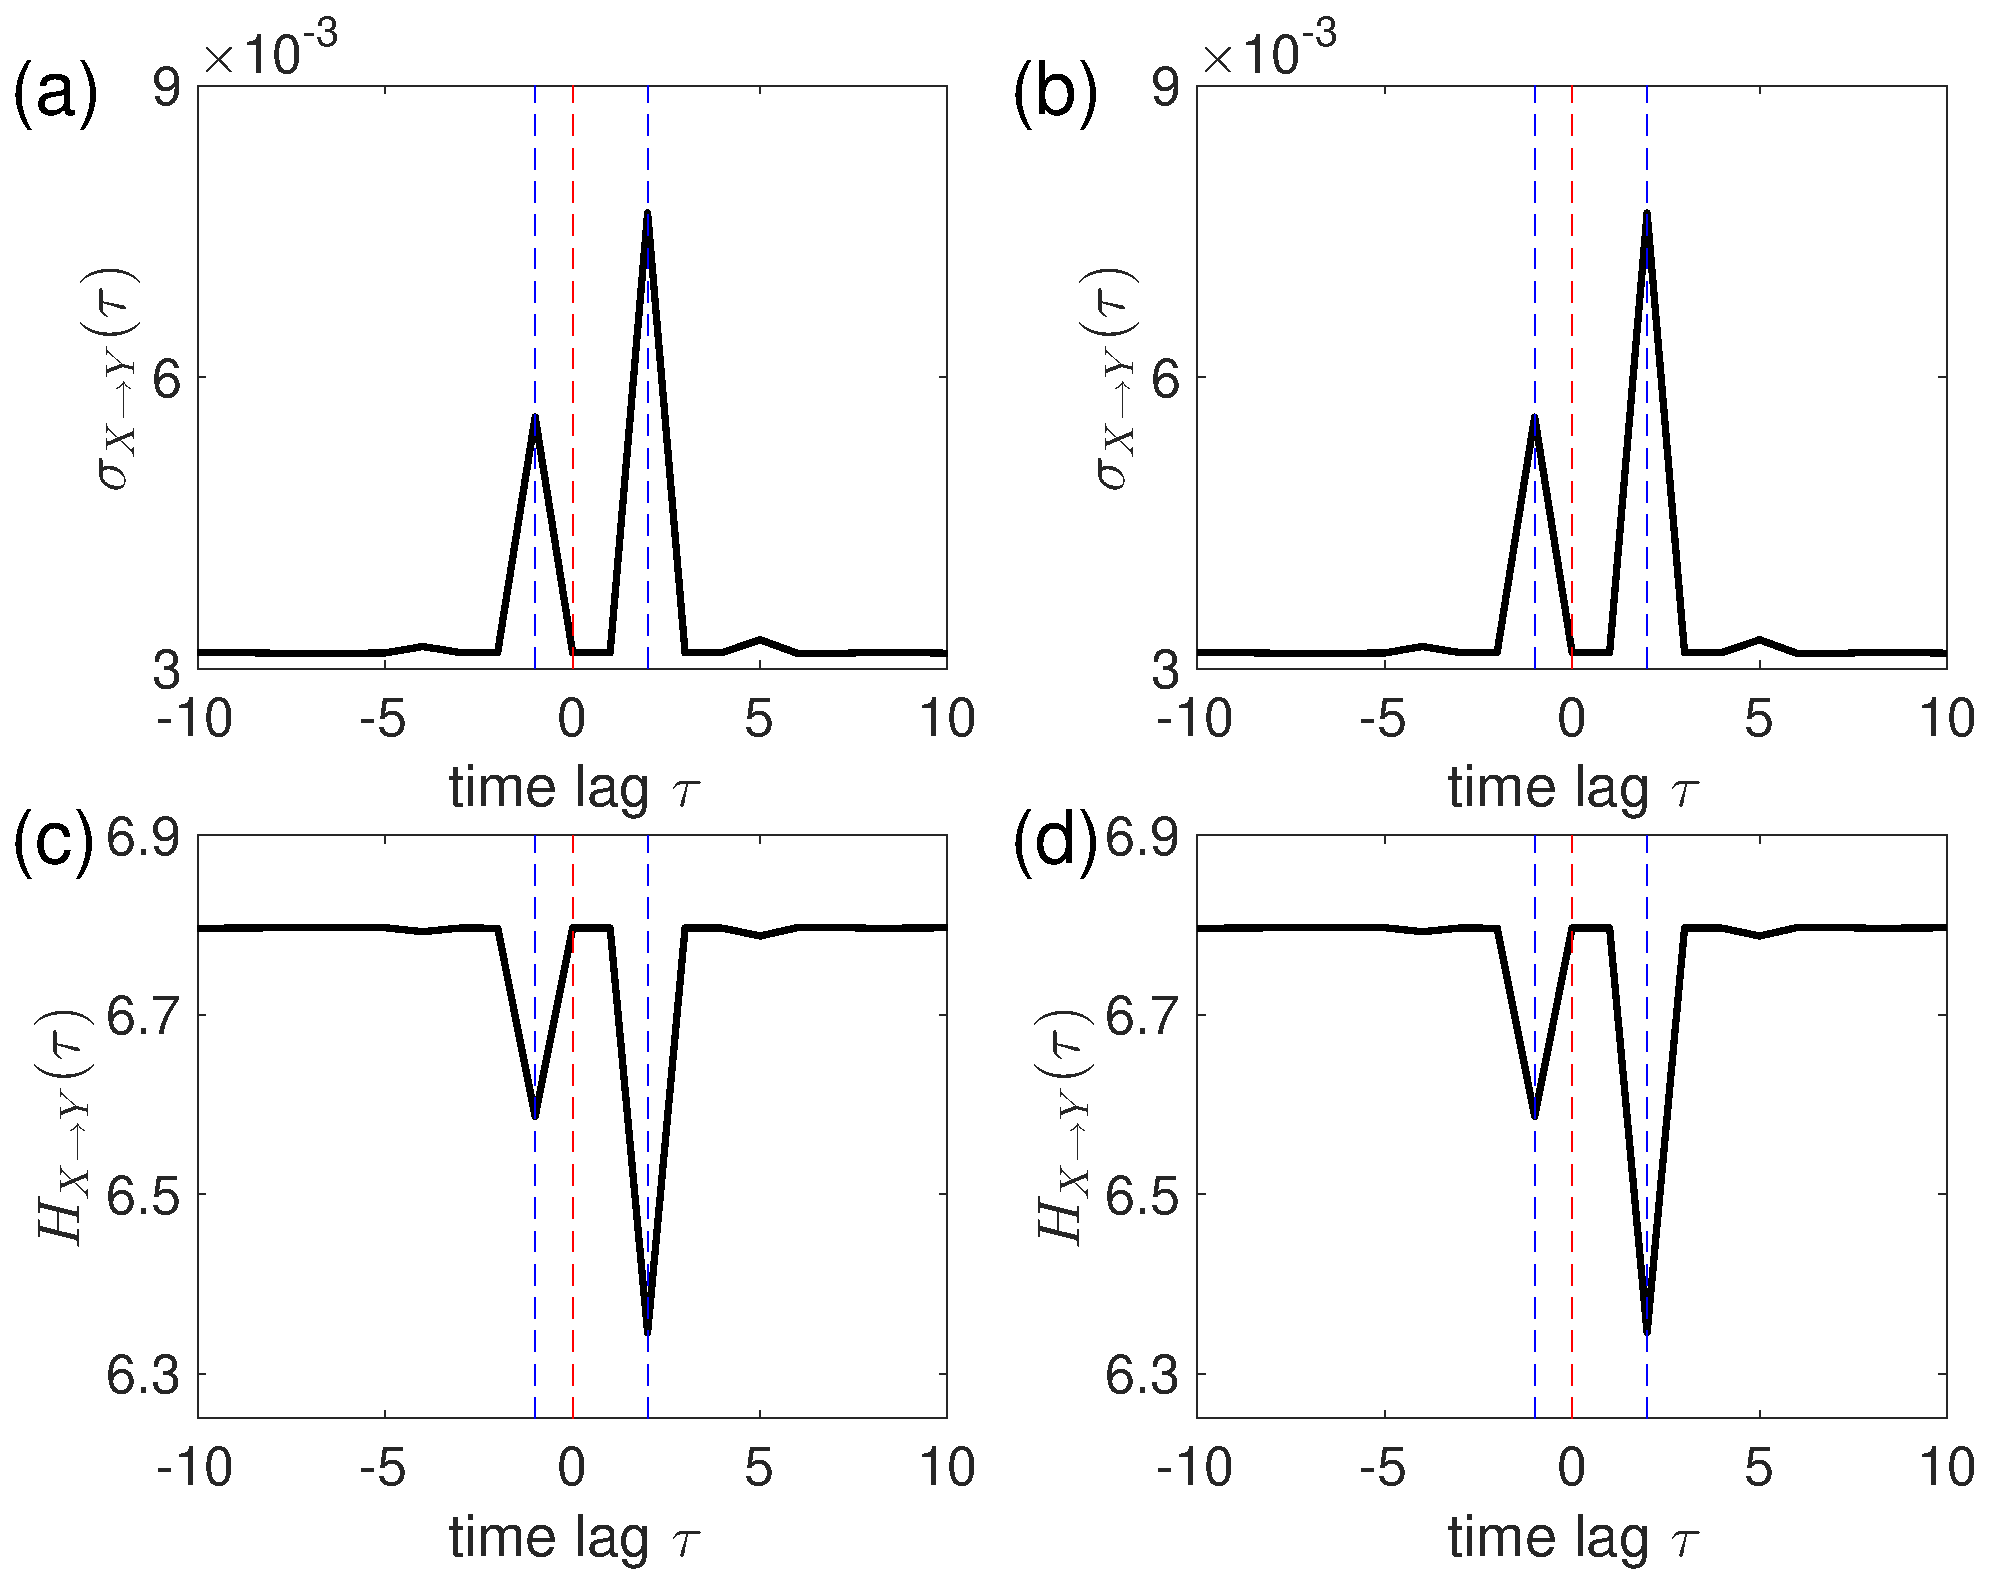
\includegraphics[width=\columnwidth]{E_E.eps}
	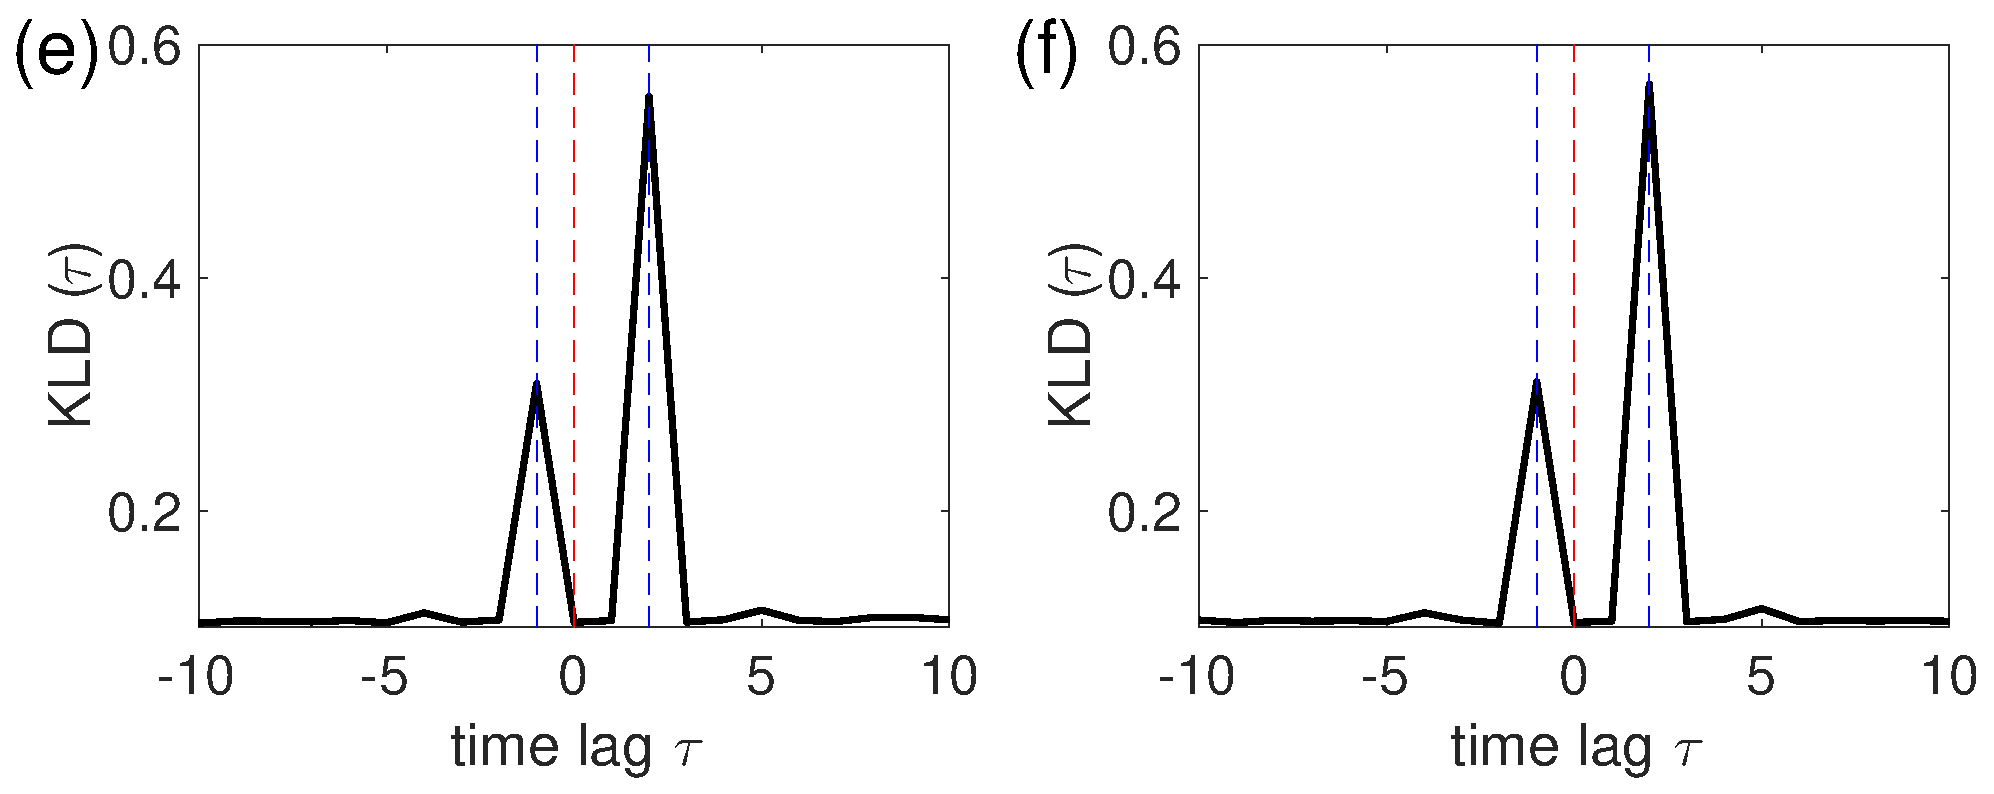
\includegraphics[width=\columnwidth]{KL_E.eps}
\caption{(Color online) Same as in Fig.~\ref{fig:stdHeqD} but for Eq.~\eqref{eq:E}. The two employed delays of $\tau = -1$ and $\tau = 2$ are additionally highlighted by vertical blue dashed lines. \label{fig:stdHeqE}}
\end{figure}

\subsection{Coupled nonlinear chaotic maps} \label{sec:henon}

As an additional numerical example, we further illustrate the performance of the proposed ordinal pattern co-occurrence complexity measures for detecting the coupling direction between two unidirectionally coupled identical nonlinear chaotic H\'enon maps~\cite{RomanoPRE2007}. In this case, the driving system $X$ reads 
\begin{equation} \label{eq:HX}
X: \left \{ \begin{aligned}
x_{t + 1}^{(1)} &= 1.4 - x^{(1)}_t x^{(1)}_t + b_1 x^{(2)}_t, \\
x_{t + 1}^{(2)} &= x_{t}^{(1)},
\end{aligned}
\right.
\end{equation}
while the response system $Y$ is given as 
\begin{equation} \label{eq:HY}
Y: \left \{ \begin{aligned}
y^{(1)}_{t + 1} &= 1.4 - [\mu x^{(1)}_t y^{(1)}_t+ (1 - \mu) y^{(1)}_t y^{(1)}_t] + b_2 y^{(2)}_t, \\
y^{(2)}_{t + 1} &= y^{(1)}_t,
\end{aligned}
\right.
\end{equation}
with $\mu$ being the coupling strength and $b_1 = b_2 = 0.3$. Following ref.~\cite{RomanoPRE2007}, we restrict our discussion to values of the coupling strength within the interval $\mu \in [0, 0.6]$, since the coupling direction cannot be identified in the presence of identical synchronization which sets in at approximately $\mu = 0.65$. Mimicking the common situation in case of real-world observational time series, we assume that we have only observed the two scalar time series $\{ x^{(1)}_t \}_{t=1}^{N}$ (system $X$) and $\{ y^{(1)}_t  \}_{t=1}^{N}$ (system $Y$) instead of the full system. The resulting series are transformed into corresponding ordinal patterns using the embedding dimension $D = 5$ and time delay $\tau_d = 100$, i.e., the same parameters as for the stochastic processes in the examples discussed in Sec.~\ref{sec:GCs}. Again, we note that the results described in the following do not change qualitatively when other reasonable choices of embedding parameters are used (not shown). 

We choose four representative coupling strengths ($\mu = 0.2, 0.3, 0.4$ and $0.5$) and show the corresponding results in Fig.~\ref{fig:stdHeqXY}. The maximum values of $\sigma_{X \to Y}$ and $\text{KLD}(\tau)$ and the minimum values of $H_{X \to Y}$ become more pronounced when the coupling strength $\mu$ increases. Our numerical results demonstrate a monotonic increase in the amplitudes of the maxima of $\sigma_{X \to Y}$ and $\text{KLD}(\tau)$ along with a monotonic decrease in the minima of $H_{X\to Y}$ when increasing the coupling strength $\mu$, which are indicated by the left (black) vertical axes of Fig.~\ref{fig:stdHeqXY}(b,d,f). Furthermore, we observe that the positions of local maxima of $\sigma_{X \to Y}$ and $\text{KLD}(\tau)$ as well as the local minima of $H_{X\to Y}$ get gradually closer to zero, which originates from the synchronization process among the two coupled systems. Notably, the positions of these maxima/minima are shifted towards zero time lag when $X$ and $Y$ are identically synchronized. We define an index $X \to Y$ to capture the coupling direction by the positions of global maxima $\tau_{max}$ of $\sigma_{X \to Y}(\tau)$ and $\text{KLD}(\tau)$ (global minima $\tau_{min}$ of $H_{X \to Y}(\tau)$), where a positive value of this index reflects a coupling direction from $X$ to $Y$. When increasing the coupling strength $\mu$ as shown by the right (blue) vertical axes in Fig.~\ref{fig:stdHeqXY}(b,d,f), we conclude that the unidirectional coupling direction from $X$ to $Y$ has been well captured by the positive values of this coupling direction index. We note that the fluctuations of this index at rather weak interactions ($\mu \in [0, 0.02]$) are due to the imprecise identification of the maxima of $\sigma_{X\to Y}(\tau)$ and $\text{KLD}(\tau)$ (minima of $H_{X\to Y}(\tau)$). In turn, the index $X \to Y$ drops to zero values when $\mu \gtrsim 0.52$ because the coupling strength gets close to the complete synchronization regime \cite{RomanoPRE2007}. 

\begin{figure}
	\centering
	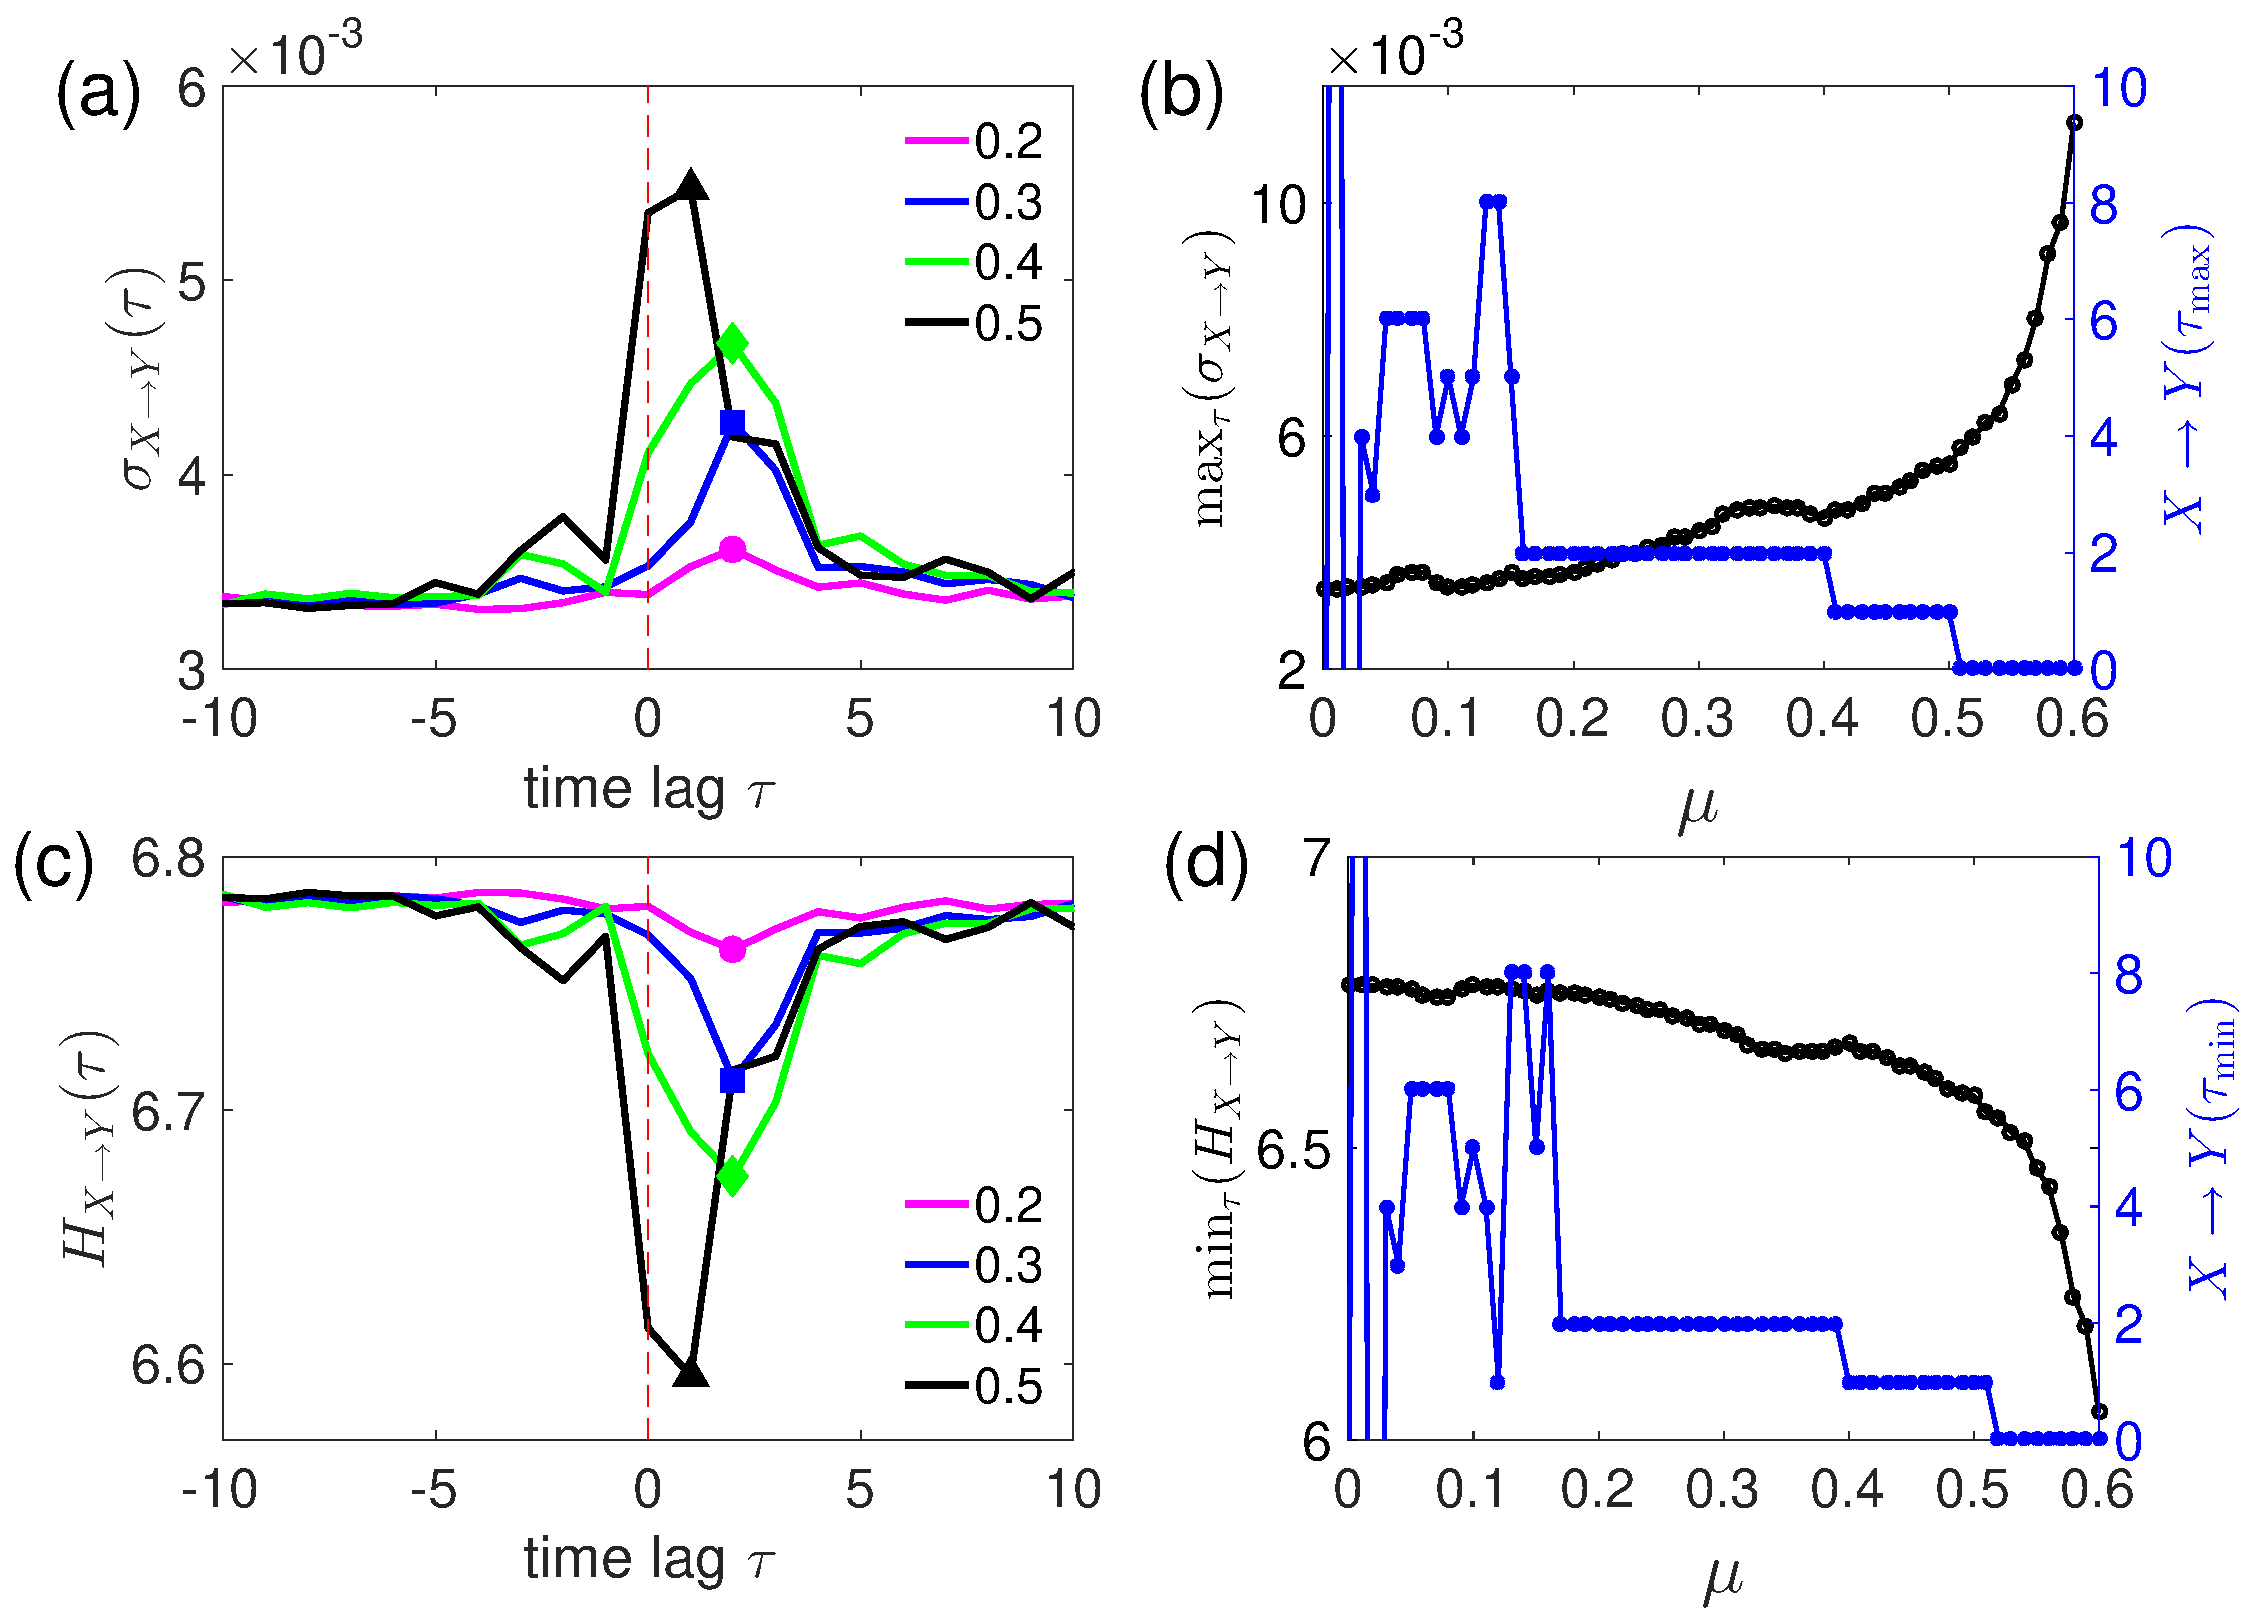
\includegraphics[width=\columnwidth]{henonMaps.eps}
	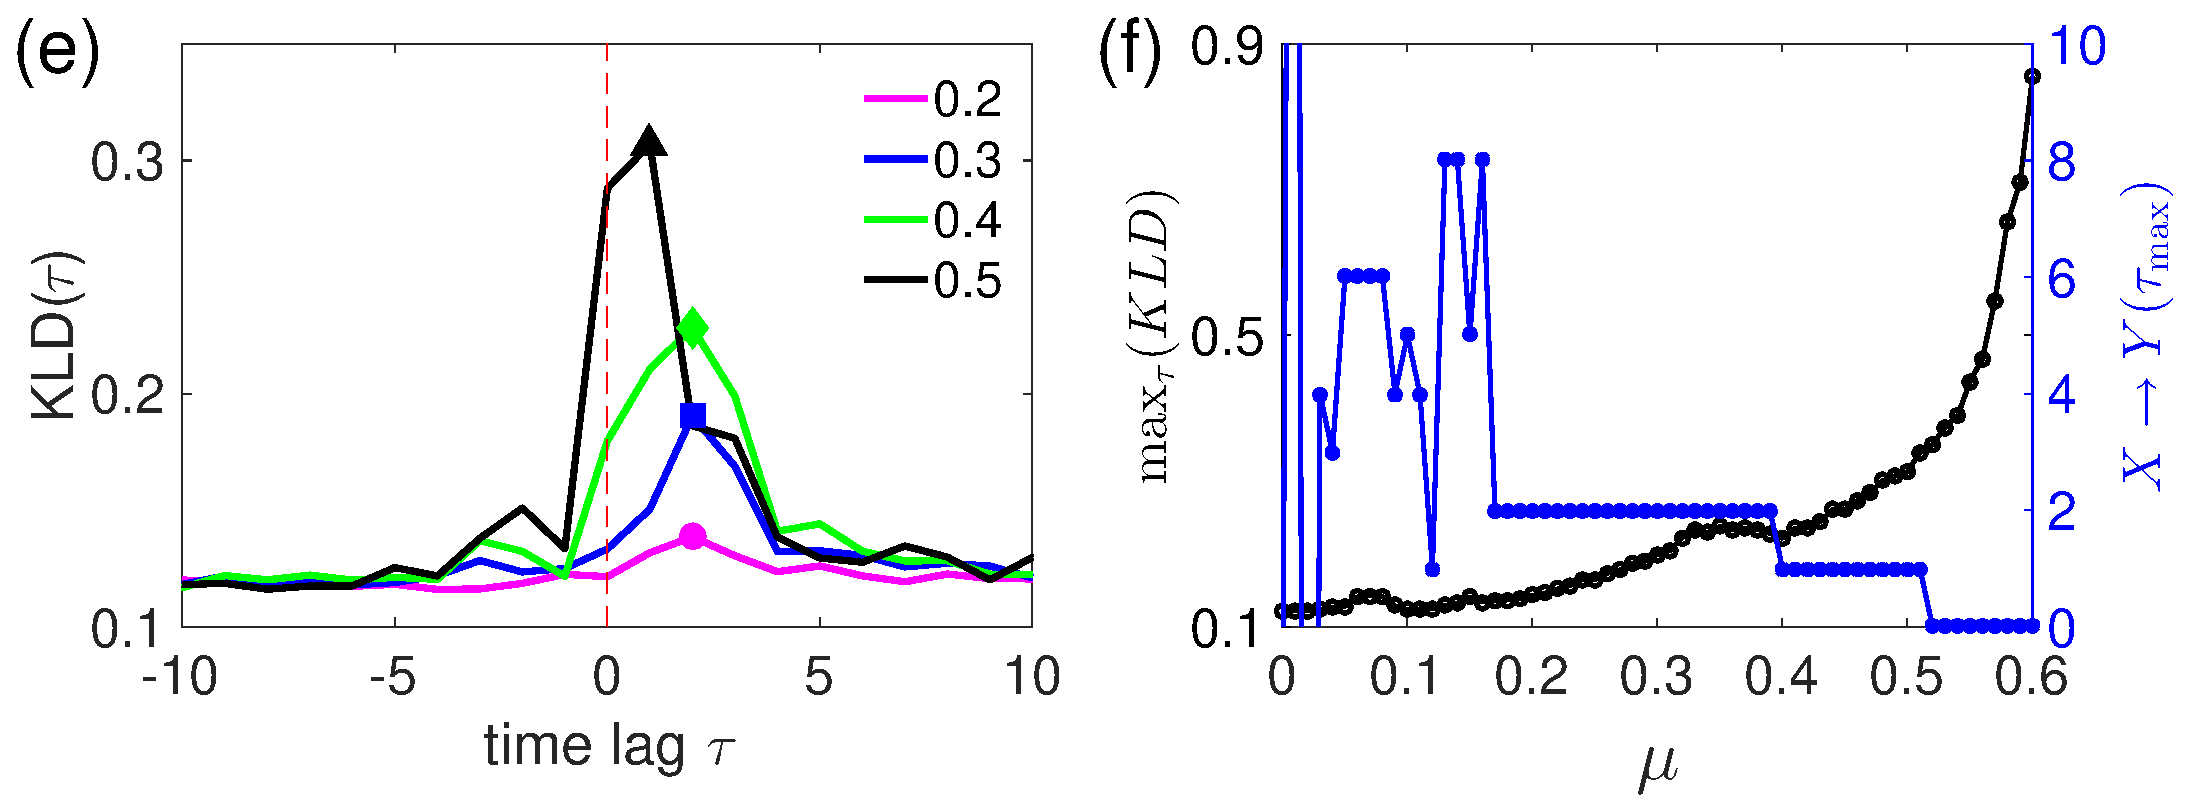
\includegraphics[width=\columnwidth]{henon_KL.eps}
\caption{(Color online) (a,c,e) Same as in Fig.~\ref{fig:stdHeqB}\textcolor{red}{(a,c,e)} but for the case of unidirectionally coupled H\'enon maps (Eqs.~\eqref{eq:HX} and \eqref{eq:HY}). We show four cases of coupling strengths $\mu = 0.2, 0.3, 0.4$ and $0.5$ as indicated by the legends. The corresponding maximum/minimum values of the three measures $\sigma_{X \to Y}$ (a), $H_{X \to Y}$ (c), and $\text{KLD}$ (e) are annotated by different types of symbols. (b,d,f) The left vertical axes indicate the maximum/minimum values of the corresponding ordinal pattern co-occurrence complexity measures while the right one provides the values of the coupling direction index $X \to Y$ (i.e., the positions of the respective maxima/minima of the three considered measures). \label{fig:stdHeqXY}}
\end{figure}


\subsection{Sample size dependence of complexity measures}

{\color{red}So far, we have shown that all three OPTN based complexity measures have been able to extract the coupling directions in our numerical examples correctly. As discussed above, $\sigma_{X\to Y}(\tau)$ is expected to be zero, while $H_{X\to Y}(\tau)$ converges to a maximal value $H_{X \to Y} = \log_2 D!$ if all $D!$ patterns are independently and uniformly distributed in both $X$ and $Y$, where independence corresponds to two uncoupled systems. These empirical expectations may be altered by non-uniform marginal probability distributions of the different patterns.}

{\color{red}In contrast to the two other measures, we do expect zero values of $\text{KLD}(\tau)$ for uncoupled systems even }if the marginal frequency distributions of the corresponding ordinal patterns are \textcolor{red}{non-uniform or} not exactly the same, \textcolor{red}{since} the KLD measure (Eqs.~\ref{eq:localKLD},\ref{eq:globalKLD}) is defined such that it should \textcolor{red}{always} asymptotically approach zero in the case of uncoupled systems. In turn, we expect positive non-zero values of KLD for two coupled systems, in particular at the positions of the true interaction delays. However, due to the finite length of any given pair of time series, one may observe small non-zero KLD values in the case of non-causal delays, as has been shown in our numerical results discussed above (cf.\ Figs.~\ref{fig:stdHeqB}-\ref{fig:stdHeqE}). 

{\color{red}In order to further study such finite sample size effects on the obtained complexity measures, we reconsider the coupled stochastic processes from Sec.~\ref{sec:GCs} and choose two specific time lags $\tau$, one corresponding to the position of the maximal values of $\sigma$ and KLD (minimal value of $H$) indicating some relevant interaction, while the other is coinciding with the position of some non-causal delay with small $\sigma$ and KLD value (large value of $H$). In the following, we report the numerical results for the KLD measure only since this discriminator should not be affected by non-uniform pattern frequency distributions. However, similar results can be obtained for the other two measures (i.e., $\sigma_{X\to Y}$ and $H_{X\to Y}$), as it is shown in Figs.~S1 and S2 in the Supplementary Materials (SM) accompanying this manuscript.}

For all four previously studied systems, we observe different asymptotic behaviors of KLD at the two \textcolor{red}{selected} delays. Notably, when increasing the time series length $N$, the KLD values at the \textcolor{red}{actual interaction} delays show convergence to non-zero values, while dropping \textcolor{red}{towards} zero approximately as $1/N$ at the non-causal delays. This feature is clearly visible for all four stochastic processes with both, unidirectional and bidirectional coupling as shown in Fig. \ref{fig:sampleSizeBCDE}. 
\begin{figure}
	\centering
	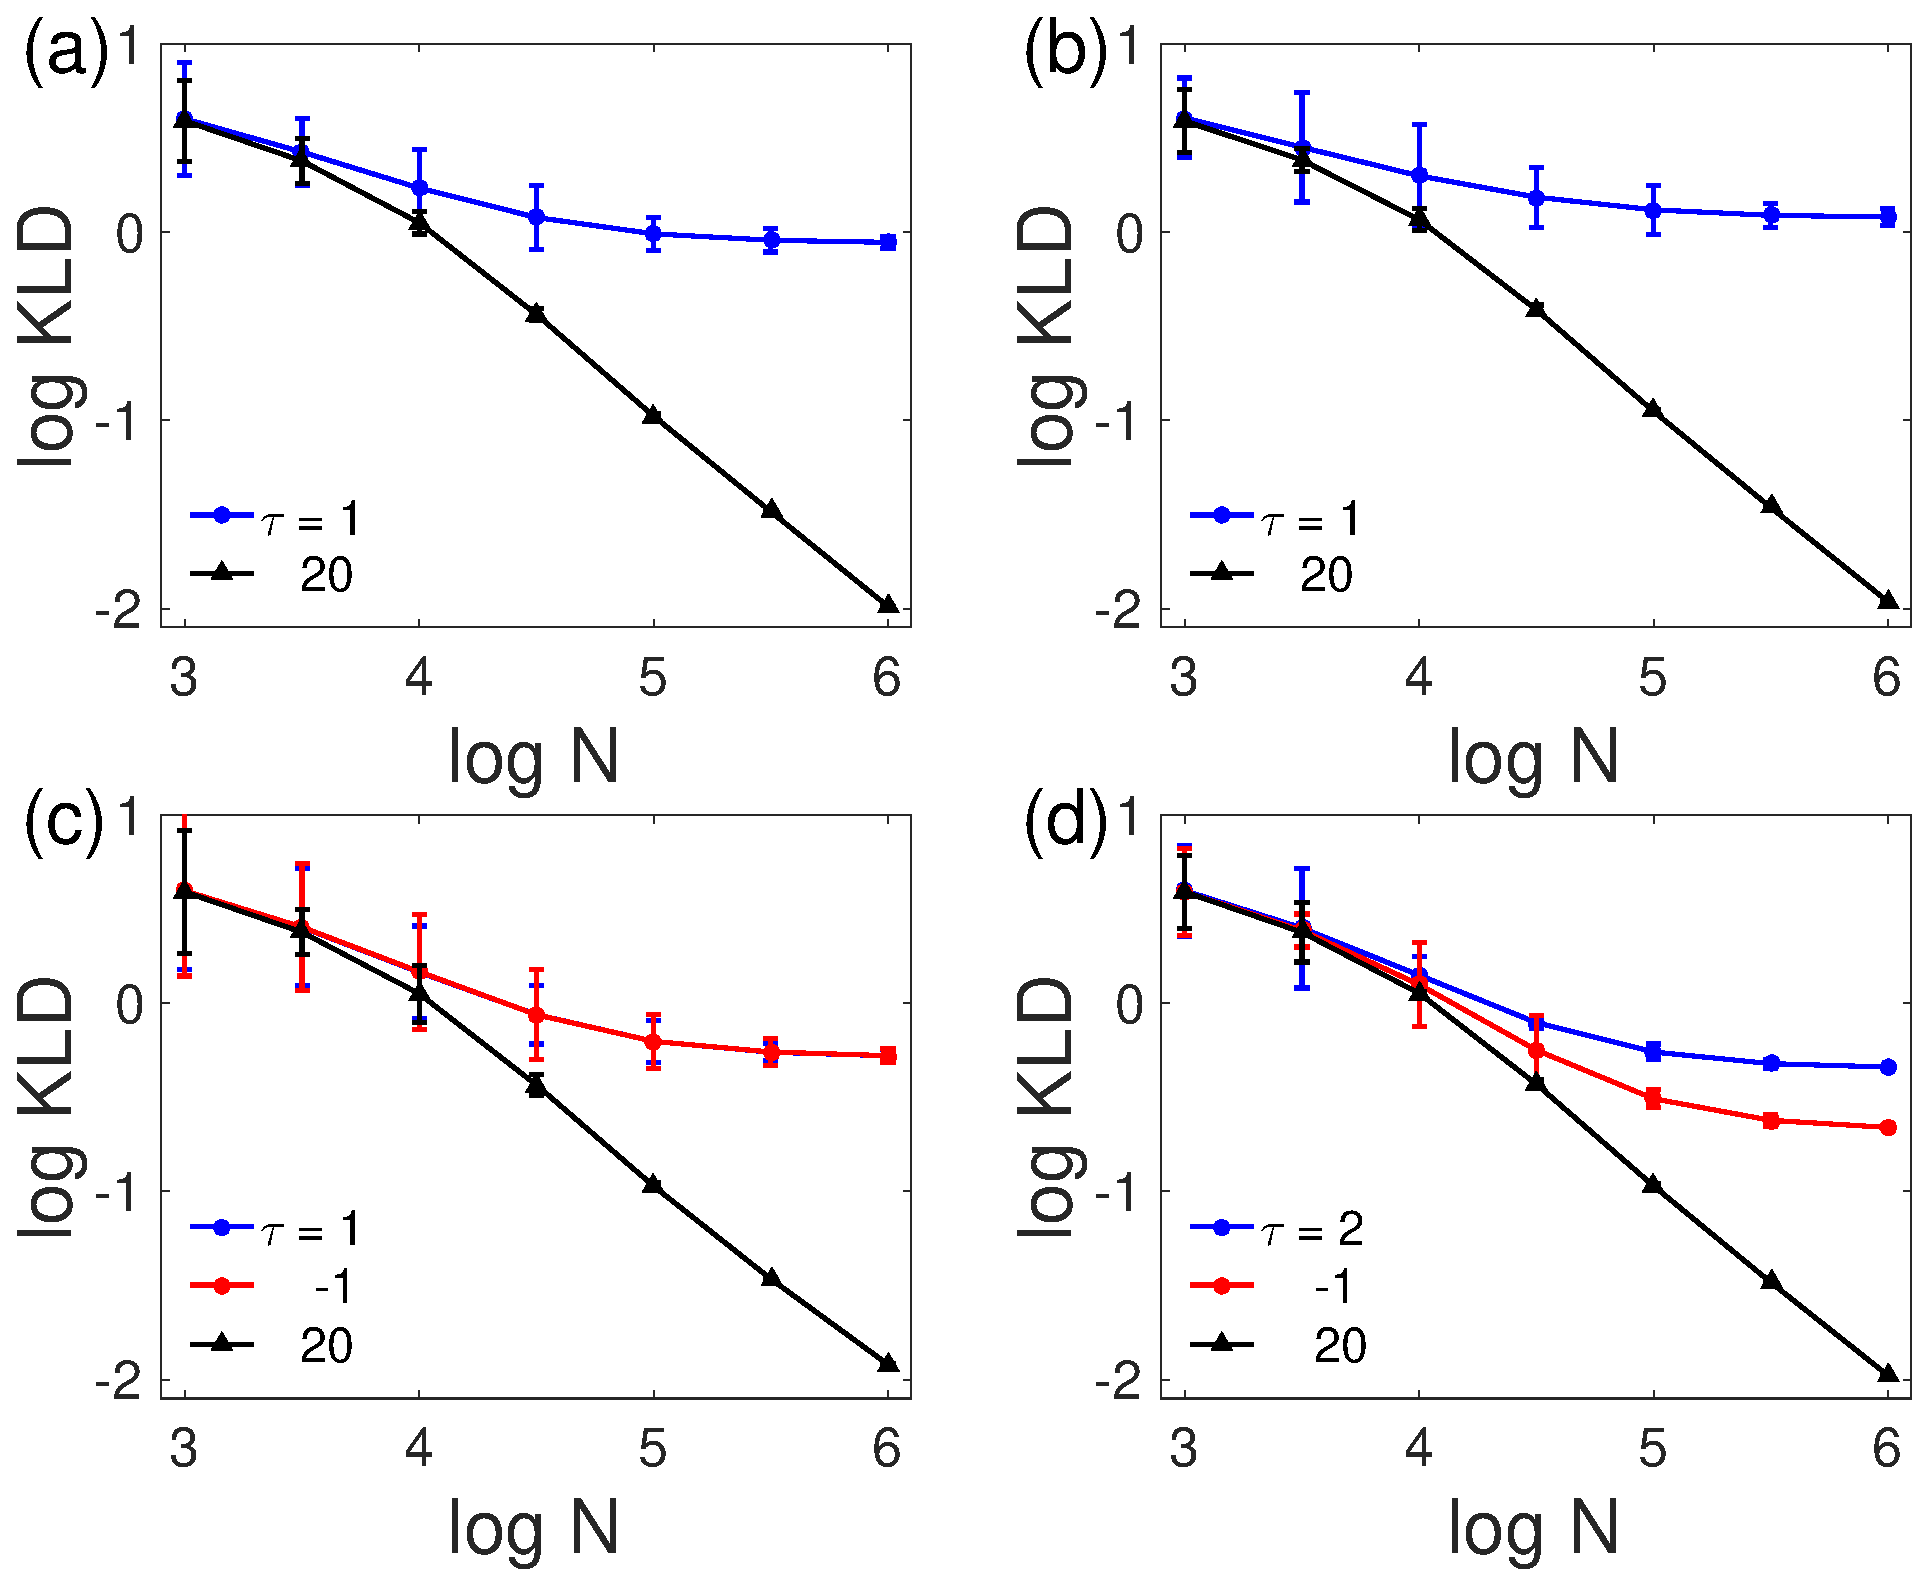
\includegraphics[width=\columnwidth]{kld_lengthBCDE.eps}
\caption{(Color online) Double logarithmic plot \textcolor{red}{(logarithms with respect to base 10)} of the dependence of KLD on the sample size $N$ for the optimal (causal) lags (blue/red) and some non-causal lag (black) for the four cases of coupled linear-stochastic systems: (a) Eq.~\eqref{eq:B} (unidirectional), (b) Eq.~\eqref{eq:C} (unidirectional), (c) Eq.~\eqref{eq:D} (symmetric bidirectional), (d) Eq.~\eqref{eq:E} (asymmetric bidirectional). In (c,d), the values for both causal delays are shown. Errorbars correspond to the standard deviation (linear scale) over 20 independent realizations.  \label{fig:sampleSizeBCDE}}
\end{figure}

{\color{red}In all cases, our convergence results are reliable if the time series length is larger than $N \gtrsim 10^4$, which may exceed the typical lengths of real-world observational time series. The main reason for this is the selected pattern order of $D=5$, which calls for $D!=120$ different nodes and, hence, $(D!)^2=14,400$ possible pairs of patterns for which mutual co-occurrence frequencies need to be estimated from the available data. For smaller pattern orders, much earlier convergence is found (see Figs.~S3--S5 in the SM), which may however come at the cost of less accuracy in the task of discriminating between actual and possibly spurious interaction delays.}  

Qualitatively equivalent results \textcolor{red}{are} obtained for the two coupled chaotic H\'enon maps from Sec.~\ref{sec:henon} as shown in Fig.~\ref{fig:sampleSizeHenon}. Here, we have again studied four different values of the coupling strength, $\mu = 0.2$, $0.3$, $0.4$ and $0.5$, and chosen the coupling delays based on the results of Fig.~\ref{fig:stdHeqXY}, corresponding to the respective maximum KLD values on the one hand, and some non-causal delay with low value of KLD on the other hand. {\color{red}As for the previously considered cases of coupled stochastic processes, the convergence results are reliable for time series of length $N \gtrsim 10^4$. A special case arises for} the rather weak coupling \textcolor{red}{of} $\mu = 0.2$, \textcolor{red}{where} the different convergence behavior of KLD \textcolor{red}{gets only} visible for $N \gtrsim 10^6$. {\color{red}Similar results have been obtained for $\sigma_{X\to Y}$ and $H_{X\to Y}$, as shown in Figs.~S6 and S7 in the SM. Again, reducing the pattern order leads to faster convergence of all three OPTN based measures for the true coupling delays, but on the cost of generally larger uncertainty (see Figs.~S8--S10 in the SM for the corresponding results for $D=4$).}
\begin{figure}
	\centering
	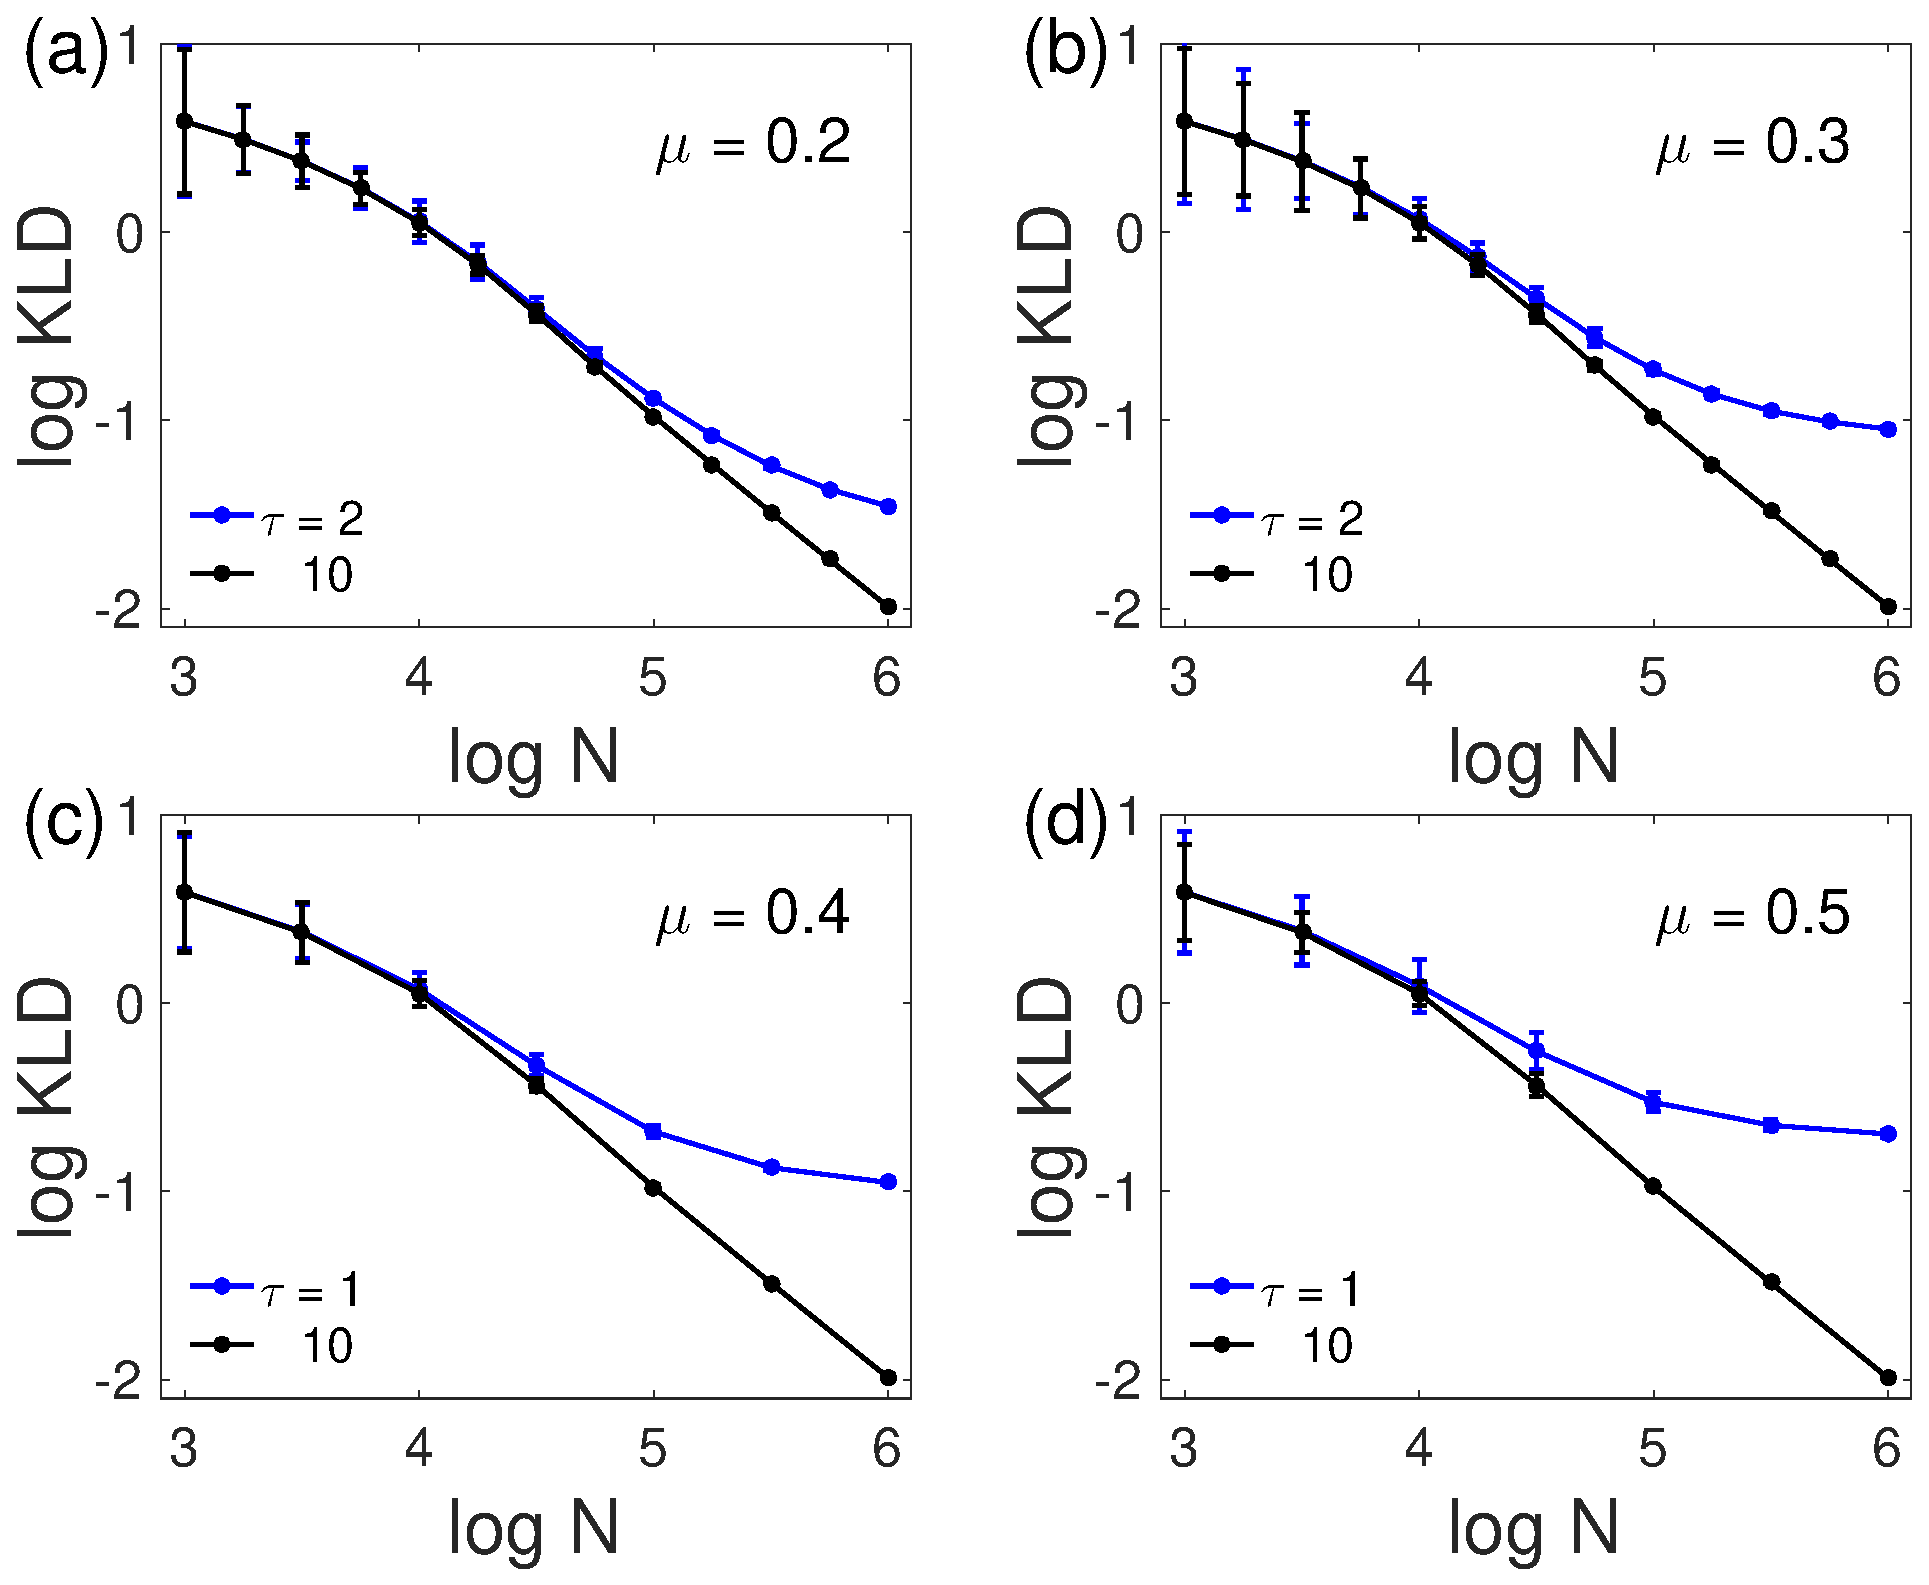
\includegraphics[width=\columnwidth]{kld_lengthHenon.eps}
\caption{(Color online) Same as in Fig. \ref{fig:sampleSizeBCDE} but for the two coupled H\'enon maps at four different coupling strengths $\mu$: (a) $\mu=0.2$ (b) $0.3$, (c) $0.4$, and (d) $0.5$. The blue lines show the behavior at the delay corresponding to maximum KLD, while the black ones show the values for a non-causal delay of $\tau=10$. \label{fig:sampleSizeHenon}}
\end{figure}

Taken together, we conclude that the small non-zero KLD values \textcolor{red}{(as well as differences of the other two OPTN complexity measures from their asymptotic values)} at non-causal delays are indeed due to the finite length of the studied time series. This suggests a straightforward strategy for obtaining confidence bounds for the computed {\color{red}complexity} values by comparing them with those for surrogate data constructed by shuffling or bootstrapping the underlying time series individually. We leave a more detailed exploration of this idea as a subject of future work.


\section{Real-world example}  \label{sec:exp}
In this section, we apply the proposed methodology to characterize the statistical interdependence between temperature records from two distant meteorological stations. Specifically, we study two long-term daily temperature records from Oxford (Great Britain) and Vienna (Austria) as previously investigated in ref.~\cite{Rybski2003} by means of phase synchronization measures. The data used here are publicly available via the KNMI Climate Explorer (\url{http://climexp.knmi.nl}) and cover the period from 1 January 1901 to 31 December 2010. Missing values have been ignored in the subsequent analysis, and the mean annual cycles (estimated by the mean temperature values of each station for a given calendar day) have been subtracted from both records to avoid the otherwise dominating effect of this regular variability mode. 

In general, temperature records like those used here are characterized by some irregular alternation between colder and warmer phases due to \textcolor{red}{synoptic circulation} patterns (corresponding to high and low pressure centers, respectively), which in the case of western-to-central Europe travel in the majority of situations in eastward direction~{\color{red}\cite{Hannachi2012,Esteban2006}}. According to the typical spatial extent of such pressure systems, it is likely that both considered sites experience similar variability patterns \textcolor{red}{(due to spatial autocorrelations in the surface air temperature field or so-called long-distance teleconnections)}, yet with some mutual delay. Indeed, Rybski \emph{et~al.}~\cite{Rybski2003} reported phase synchronization between both stations with the record obtained in Oxford leading that from Vienna by on average 1 day. It should be noted, however, that one should not expect a simple strong linear correlation between both series, since the typical climatology at both sites is clearly different (i.e., more marine -- and, hence, variable -- versus more continental -- and, hence, persistent) and potentially affected by different circulation regimes.

Taking the two temperature series as described above, we construct the corresponding bipartite OPTN. Subsequently, we compute the transition complexity measures $\sigma_{X\to Y}$, $H_{X\to Y}$ and $\text{KLD}_{X\to Y}$ for different time lags, which are shown in Fig.~\ref{fig:stdHeqTemp}(a)-(c). When mutually shifting both series with respect to each other by several days in any of the two possible directions, we find a marked yet relatively slow decrease of $\sigma_{X\to Y} (\tau)$, $H_{X\to Y} (\tau)$ and $\text{KLD}_{X\to Y}$, which can most likely be explained by the known persistence of air temperature time series~{\color{red}\cite{Bunde1998}}, together with the expectation that the actual delay should be time-dependent and, thus, distributed over several values. Altogether, the most significant values of all three measures are attained at a mutual delay of $\tau=1$ day, with the values at $\tau=2$ days being only slightly less prominent. In summary, our analysis identifies an interaction delay between the respective local temperature variations of 1 to 2 days (with Oxford leading Vienna), which is consistent with the previous results of phase synchronization analysis~\cite{Rybski2003}. 

\textcolor{red}{In order to put the estimated coupling delay into a meteorological context, we note that the actual travel direction and speed of synoptic-scale atmospheric patterns over Europe varies greatly over the year~\cite{Esteban2006}. However, westwind patterns are generally most frequently observed. Given a distance between the two stations in Oxford and Vienna of about 1,300 km, we may associate the inferred coupling delay of 1 to 2 days with a typical zonal (westward) propagation speed of such atmospheric patterns over Western and Central Europe of the order of 30 to 60 km/h, which appears not unreasonable given everyday experience. Of course, the actual values at specific points in time and space will vary greatly (e.g., storms travel with much larger speed, while we may observe almost no zonal dynamics in case of northerly or southerly winds, or even eastward propagation in relatively rare cases). This great variety of synoptic weather situations thus leads to a strongly time-dependent travel time of an air parcel starting at Oxford until reaching its closest distance to Vienna, which explains our observation of not a single sharply defined coupling delay, but rather some broad distribution of possible delays.}

\begin{figure}
	\centering
	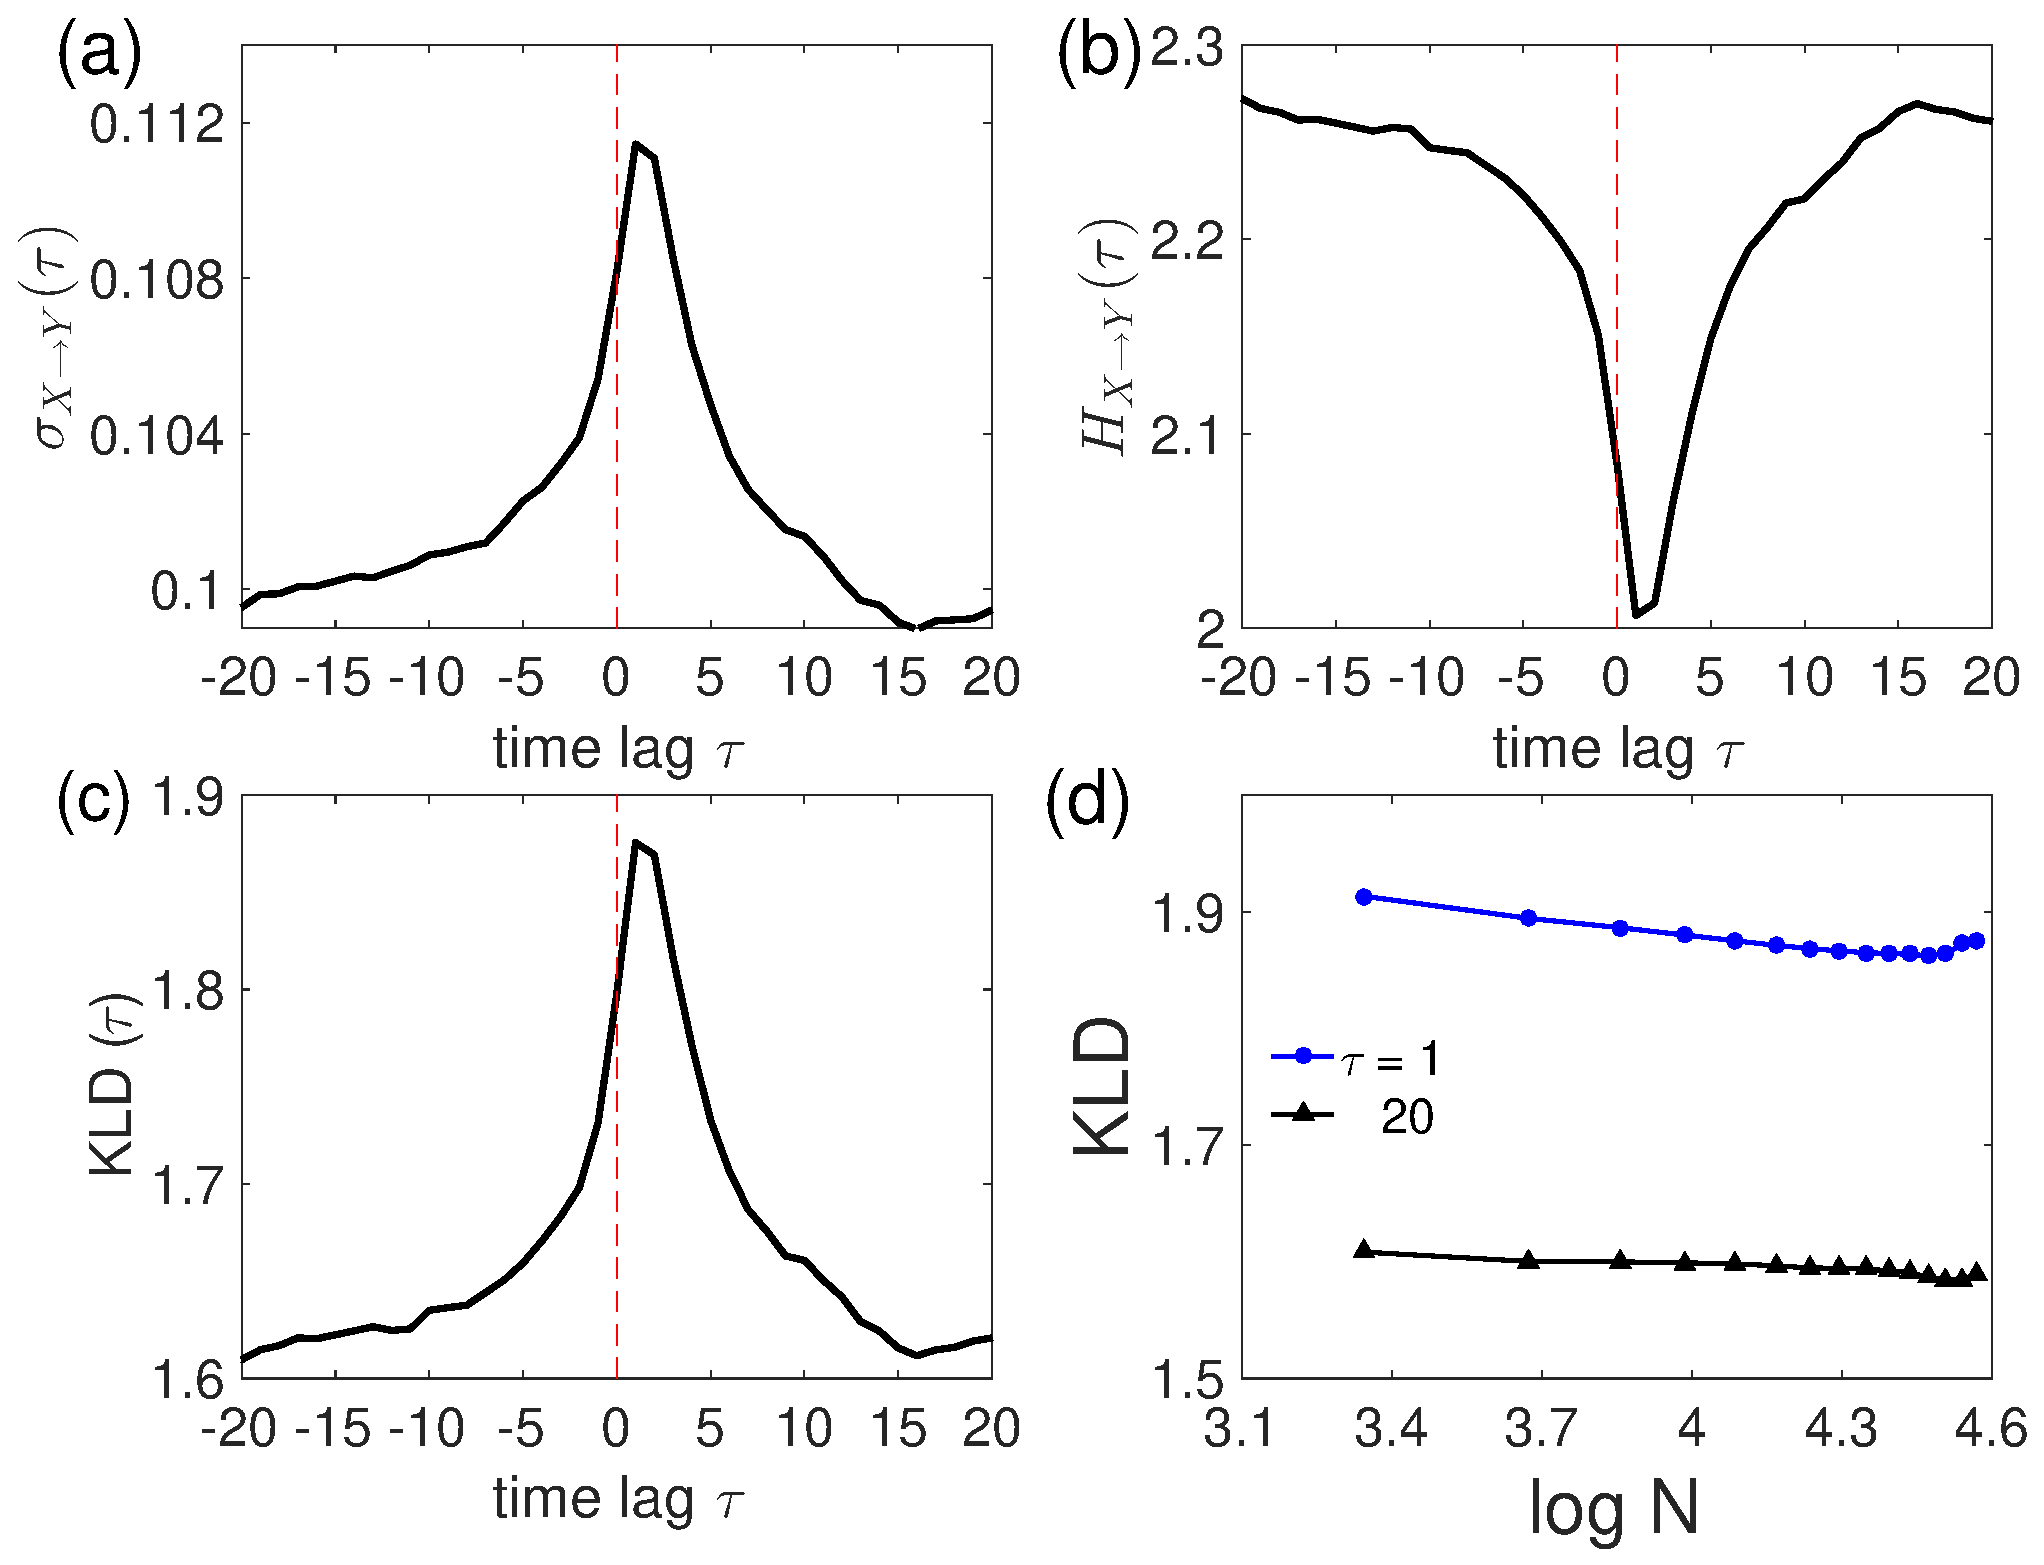
\includegraphics[width=\columnwidth]{E_temperature.eps}
\caption{(Color online) OPTN based statistical coupling indicators between the daily surface air temperature records from Oxford ($X$) and Vienna ($Y$): (a) mean squared deviations of the conditional co-occurrence frequencies of ordinal patterns $\sigma_{X\to Y} (\tau)$, (b) global ordinal pattern co-occurrence entropy $H_{X\to Y}(\tau)$, and (c) Kullback-Leibler divergence $\text{KLD}(\tau)$. Dashed red vertical lines indicate the values for possible instantaneous interactions. (d) Dependence of KLD on the sample length $N$ at the optimal delay ($\tau=1$ day, blue) and some arbitrarily chosen large delay ($\tau=20$ days, black). 
\label{fig:stdHeqTemp}}
\end{figure}

In addition to the identification of the expected interaction delay between both temperature records, we have again studied the effect of the time series length on the estimated OPTN based coupling indicators for the example of KLD. For this purpose, pairs of time series values have been selected at random to form subsamples of arbitrary sizes. This kind of cross-validation procedure demonstrates the saturation of the obtained estimates at sufficiently large sample sizes (Fig.~\ref{fig:stdHeqTemp}(d)). Most importantly, the KLD values at the optimal interaction delay of $\tau=1$ day are consistently larger than those at any other delay that would not be justified by the underlying meteorological processes. However, there is a non-zero statistical relationship between both records even at a delay of 20 days, which is manifested in the saturation of KLD for this delay with increasing time series length $N$ instead of a gradual decrease as previously observed in our numerical model examples. {\color{red}Similar results have been obtained for $\sigma_{X\to Y}$ and $H_{X\to Y}$, as shown in Fig.~S11 in the SM.}

\section{Conclusions} \label{sec:con}

In summary, we have proposed to infer coupling direction and strength among pairs of dynamical systems by computing complexity measures \textcolor{red}{based upon} the resulting bipartite ordinal {\color{red}partition} transition networks (OPTNs). More specifically, we have estimated three quantitative characteristics capturing different aspects of the heterogeneity of conditional frequencies of occurrences in one time series relative to the second one. The first two measures, $\sigma_{X\to Y}$ and $H_{X\to Y}$, both characterize the degree to which the ordinal pattern distribution in one series can be attributed to prior information from the ordinal patterns of the second one. By contrast, the Kullback-Leibler divergence (KLD) between the conditional probability distribution of ordinal patterns $p(\pi_{j}^{Y} | \pi_i^{X})$ and the corresponding marginals $p(\pi_j^{Y})$ directly characterizes the presence of interdependence between the two underlying systems $X$ and $Y$. 

In order to identify the direction and relevant delay of coupling, we have performed a time-lagged analysis using all three measures, where the ordinal pattern series have been shifted relative \textcolor{red}{to} each other by a given time delay $\tau$ prior to evaluating the associated empirical co-occurrence frequencies. Numerical results for unidirectionally and bidirectionally coupled stochastic processes and H\'enon maps have demonstrated the existence of pronounced signatures at the respective interaction delays, capturing the prescribed coupling directions successfully. In the particular case of coupling analysis for two temperature records from Oxford and Vienna, the ordinal pattern co-occurrence complexity measures have consistently identified interactions at a delay of 1 to 2 days, which suggests that these measures can be useful for analyzing interactions among real-world (noisy) time series. Follow-up studies should take up this problem to address more systematically the effect of observational noise on coupling identification using OPTN based complexity measures as compared to other existing statistical approaches serving similar purposes. The present work has provided a proof-of-concept that concepts from ordinal time series analysis, combined with ideas from complex network theory, can provide complementary tools for coupling analysis. However, we have not attempted to study the performance of these measures along with that of other existing techniques, which remains a subject of future studies.

Further open challenges along these lines of research include, but are not limited to characterizing dynamic variations of the coupling direction, i.e., situations where coupling changes its strength and possibly even direction as time evolves. A sliding window technique may be an option for such studies, however, the construction of proper OPTNs could be affected by the window sizes (relative to the time scales at which the coupling changes), which requires reliable estimation of the considered OPTN complexity measures. In addition, the generalization of the proposed measures to the case of more than two interacting processes is interesting, since complex interaction schemes are frequently observed across a vast range of scientific disciplines. Along with such examples, for instance, distinguishing direct from indirect coupling among three of more mutually coupled systems is still a subject of active research, which could be extended to further applications of OPTNs. 

\section*{Supplementary Material}
See supplementary material for the complete list of figures of the sample size dependence of complexity measures. 

\section*{Acknowledgement}
Parts of this work have been financially supported by the National Natural Science Foundation of China (Grant No. 11872182, 11875132, and 11835003) and the Natural Science Foundation of Shanghai (Grant No. 17ZR1444800 and 18ZR1411800). RVD acknowledges funding by the IRTG 1740/TRP 2011/50151-0 (funded by the DFG and FAPESP) and by the German Federal Ministry for Education and Research (BMBF) via the BMBF Young Investigators Group $\text{CoSy-CC}^2$: Complex Systems Approaches to Understanding Causes and Consequences of Past, Present and Future Climate Change (grant no. 01LN1306A).

%\bibliographystyle{unsrt}
%\bibliography{PhysRep2018N,ref_Zhang,ref_reik}
%merlin.mbs aipnum4-1.bst 2010-07-25 4.21a (PWD, AO, DPC) hacked
%Control: key (0)
%Control: author (8) initials jnrlst
%Control: editor formatted (1) identically to author
%Control: production of article title (0) allowed
%Control: page (1) range
%Control: year (1) truncated
%Control: production of eprint (0) enabled
\begin{thebibliography}{49}%
\makeatletter
\providecommand \@ifxundefined [1]{%
 \@ifx{#1\undefined}
}%
\providecommand \@ifnum [1]{%
 \ifnum #1\expandafter \@firstoftwo
 \else \expandafter \@secondoftwo
 \fi
}%
\providecommand \@ifx [1]{%
 \ifx #1\expandafter \@firstoftwo
 \else \expandafter \@secondoftwo
 \fi
}%
\providecommand \natexlab [1]{#1}%
\providecommand \enquote  [1]{``#1''}%
\providecommand \bibnamefont  [1]{#1}%
\providecommand \bibfnamefont [1]{#1}%
\providecommand \citenamefont [1]{#1}%
\providecommand \href@noop [0]{\@secondoftwo}%
\providecommand \href [0]{\begingroup \@sanitize@url \@href}%
\providecommand \@href[1]{\@@startlink{#1}\@@href}%
\providecommand \@@href[1]{\endgroup#1\@@endlink}%
\providecommand \@sanitize@url [0]{\catcode `\\12\catcode `\$12\catcode
  `\&12\catcode `\#12\catcode `\^12\catcode `\_12\catcode `\%12\relax}%
\providecommand \@@startlink[1]{}%
\providecommand \@@endlink[0]{}%
\providecommand \url  [0]{\begingroup\@sanitize@url \@url }%
\providecommand \@url [1]{\endgroup\@href {#1}{\urlprefix }}%
\providecommand \urlprefix  [0]{URL }%
\providecommand \Eprint [0]{\href }%
\providecommand \doibase [0]{http://dx.doi.org/}%
\providecommand \selectlanguage [0]{\@gobble}%
\providecommand \bibinfo  [0]{\@secondoftwo}%
\providecommand \bibfield  [0]{\@secondoftwo}%
\providecommand \translation [1]{[#1]}%
\providecommand \BibitemOpen [0]{}%
\providecommand \bibitemStop [0]{}%
\providecommand \bibitemNoStop [0]{.\EOS\space}%
\providecommand \EOS [0]{\spacefactor3000\relax}%
\providecommand \BibitemShut  [1]{\csname bibitem#1\endcsname}%
\let\auto@bib@innerbib\@empty
%</preamble>
\bibitem [{\citenamefont {Bradley}\ and\ \citenamefont
  {Kantz}(2015)}]{Bradley2015c}%
  \BibitemOpen
  \bibfield  {author} {\bibinfo {author} {\bibfnamefont {E.}~\bibnamefont
  {Bradley}}\ and\ \bibinfo {author} {\bibfnamefont {H.}~\bibnamefont
  {Kantz}},\ }\bibfield  {title} {\enquote {\bibinfo {title} {{Nonlinear
  time-series analysis revisited}},}\ }\href {\doibase 10.1063/1.4917289}
  {\bibfield  {journal} {\bibinfo  {journal} {Chaos}\ }\textbf {\bibinfo
  {volume} {25}},\ \bibinfo {pages} {097610} (\bibinfo {year} {2015})},\
  \Eprint {http://arxiv.org/abs/1503.07493} {arXiv:1503.07493} \BibitemShut
  {NoStop}%
\bibitem [{\citenamefont {Kantz}\ and\ \citenamefont
  {Schreiber}(2004)}]{Kantz97}%
  \BibitemOpen
  \bibfield  {author} {\bibinfo {author} {\bibfnamefont {H.}~\bibnamefont
  {Kantz}}\ and\ \bibinfo {author} {\bibfnamefont {T.}~\bibnamefont
  {Schreiber}},\ }\href@noop {} {\emph {\bibinfo {title} {Nonlinear Time Series
  Analysis}}},\ \bibinfo {edition} {2nd}\ ed.\ (\bibinfo  {publisher}
  {Cambridge University Press, Cambridge},\ \bibinfo {year} {2004})\BibitemShut
  {NoStop}%
\bibitem [{\citenamefont {Zou}\ \emph {et~al.}(2019)\citenamefont {Zou},
  \citenamefont {Donner}, \citenamefont {Marwan}, \citenamefont {Donges},\ and\
  \citenamefont {Kurths}}]{ZouPR2018}%
  \BibitemOpen
  \bibfield  {author} {\bibinfo {author} {\bibfnamefont {Y.}~\bibnamefont
  {Zou}}, \bibinfo {author} {\bibfnamefont {R.~V.}\ \bibnamefont {Donner}},
  \bibinfo {author} {\bibfnamefont {N.}~\bibnamefont {Marwan}}, \bibinfo
  {author} {\bibfnamefont {J.~F.}\ \bibnamefont {Donges}}, \ and\ \bibinfo
  {author} {\bibfnamefont {J.}~\bibnamefont {Kurths}},\ }\bibfield  {title}
  {\enquote {\bibinfo {title} {Complex network approaches to nonlinear time
  series analysis},}\ }\href {\doibase 10.1016/j.physrep.2018.10.005}
  {\bibfield  {journal} {\bibinfo  {journal} {Physics Reports}\ }\textbf
  {\bibinfo {volume} {787}},\ \bibinfo {pages} {1--97} (\bibinfo {year}
  {2019})}\BibitemShut {NoStop}%
\bibitem [{\citenamefont {Marwan}\ \emph {et~al.}(2009)\citenamefont {Marwan},
  \citenamefont {Donges}, \citenamefont {Zou}, \citenamefont {Donner},\ and\
  \citenamefont {Kurths}}]{Marwan2009}%
  \BibitemOpen
  \bibfield  {author} {\bibinfo {author} {\bibfnamefont {N.}~\bibnamefont
  {Marwan}}, \bibinfo {author} {\bibfnamefont {J.~F.}\ \bibnamefont {Donges}},
  \bibinfo {author} {\bibfnamefont {Y.}~\bibnamefont {Zou}}, \bibinfo {author}
  {\bibfnamefont {R.~V.}\ \bibnamefont {Donner}}, \ and\ \bibinfo {author}
  {\bibfnamefont {J.}~\bibnamefont {Kurths}},\ }\bibfield  {title} {\enquote
  {\bibinfo {title} {{Complex network approach for recurrence analysis of time
  series}},}\ }\href {\doibase 10.1016/j.physleta.2009.09.042} {\bibfield
  {journal} {\bibinfo  {journal} {Phys. Lett. A}\ }\textbf {\bibinfo {volume}
  {373}},\ \bibinfo {pages} {4246--4254} (\bibinfo {year} {2009})},\ \Eprint
  {http://arxiv.org/abs/0907.3368} {arXiv:0907.3368} \BibitemShut {NoStop}%
\bibitem [{\citenamefont {Donner}\ \emph {et~al.}(2010)\citenamefont {Donner},
  \citenamefont {Zou}, \citenamefont {Donges}, \citenamefont {Marwan},\ and\
  \citenamefont {Kurths}}]{Donner2010NJP}%
  \BibitemOpen
  \bibfield  {author} {\bibinfo {author} {\bibfnamefont {R.~V.}\ \bibnamefont
  {Donner}}, \bibinfo {author} {\bibfnamefont {Y.}~\bibnamefont {Zou}},
  \bibinfo {author} {\bibfnamefont {J.~F.}\ \bibnamefont {Donges}}, \bibinfo
  {author} {\bibfnamefont {N.}~\bibnamefont {Marwan}}, \ and\ \bibinfo {author}
  {\bibfnamefont {J.}~\bibnamefont {Kurths}},\ }\bibfield  {title} {\enquote
  {\bibinfo {title} {Recurrence networks -- {A} novel paradigm for nonlinear
  time series analysis},}\ }\href {\doibase 10.1088/1367-2630/12/3/033025}
  {\bibfield  {journal} {\bibinfo  {journal} {New J. Phys.}\ }\textbf {\bibinfo
  {volume} {12}},\ \bibinfo {pages} {033025} (\bibinfo {year}
  {2010})}\BibitemShut {NoStop}%
\bibitem [{\citenamefont {Lacasa}\ \emph {et~al.}(2008)\citenamefont {Lacasa},
  \citenamefont {Luque}, \citenamefont {Ballesteros}, \citenamefont {Luque},\
  and\ \citenamefont {Nuno}}]{Lacasa2008}%
  \BibitemOpen
  \bibfield  {author} {\bibinfo {author} {\bibfnamefont {L.}~\bibnamefont
  {Lacasa}}, \bibinfo {author} {\bibfnamefont {B.}~\bibnamefont {Luque}},
  \bibinfo {author} {\bibfnamefont {F.}~\bibnamefont {Ballesteros}}, \bibinfo
  {author} {\bibfnamefont {J.}~\bibnamefont {Luque}}, \ and\ \bibinfo {author}
  {\bibfnamefont {J.~C.}\ \bibnamefont {Nuno}},\ }\bibfield  {title} {\enquote
  {\bibinfo {title} {{From time series to complex networks: The visibility
  graph}},}\ }\href {\doibase 10.1073/pnas.0709247105} {\bibfield  {journal}
  {\bibinfo  {journal} {Proc. Natl. Acad. Sci.}\ }\textbf {\bibinfo {volume}
  {105}},\ \bibinfo {pages} {4972--4975} (\bibinfo {year} {2008})},\ \Eprint
  {http://arxiv.org/abs/0810.0920} {arXiv:0810.0920} \BibitemShut {NoStop}%
\bibitem [{\citenamefont {Nicolis}, \citenamefont {Cantu},\ and\ \citenamefont
  {Nicolis}(2005)}]{Nicolis2005}%
  \BibitemOpen
  \bibfield  {author} {\bibinfo {author} {\bibfnamefont {G.}~\bibnamefont
  {Nicolis}}, \bibinfo {author} {\bibfnamefont {A.~G.}\ \bibnamefont {Cantu}},
  \ and\ \bibinfo {author} {\bibfnamefont {C.}~\bibnamefont {Nicolis}},\
  }\bibfield  {title} {\enquote {\bibinfo {title} {{Dynamical aspects of
  interaction networks}},}\ }\href {\doibase 10.1142/S0218127405014167}
  {\bibfield  {journal} {\bibinfo  {journal} {Int. J. Bifurc. Chaos}\ }\textbf
  {\bibinfo {volume} {15}},\ \bibinfo {pages} {3467--3480} (\bibinfo {year}
  {2005})}\BibitemShut {NoStop}%
\bibitem [{\citenamefont {McCullough}\ \emph {et~al.}(2015)\citenamefont
  {McCullough}, \citenamefont {Small}, \citenamefont {Stemler},\ and\
  \citenamefont {Iu}}]{McCullough2015}%
  \BibitemOpen
  \bibfield  {author} {\bibinfo {author} {\bibfnamefont {M.}~\bibnamefont
  {McCullough}}, \bibinfo {author} {\bibfnamefont {M.}~\bibnamefont {Small}},
  \bibinfo {author} {\bibfnamefont {T.}~\bibnamefont {Stemler}}, \ and\
  \bibinfo {author} {\bibfnamefont {H.~H.-H.}\ \bibnamefont {Iu}},\ }\bibfield
  {title} {\enquote {\bibinfo {title} {{Time lagged ordinal partition networks
  for capturing dynamics of continuous dynamical systems}},}\ }\href {\doibase
  10.1063/1.4919075} {\bibfield  {journal} {\bibinfo  {journal} {Chaos}\
  }\textbf {\bibinfo {volume} {25}},\ \bibinfo {pages} {053101} (\bibinfo
  {year} {2015})},\ \Eprint {http://arxiv.org/abs/arXiv:1501.06656v1}
  {arXiv:arXiv:1501.06656v1} \BibitemShut {NoStop}%
\bibitem [{\citenamefont {Zhang}\ and\ \citenamefont
  {Small}(2006)}]{Zhang2006}%
  \BibitemOpen
  \bibfield  {author} {\bibinfo {author} {\bibfnamefont {J.}~\bibnamefont
  {Zhang}}\ and\ \bibinfo {author} {\bibfnamefont {M.}~\bibnamefont {Small}},\
  }\bibfield  {title} {\enquote {\bibinfo {title} {{Complex Network from
  Pseudoperiodic Time Series: Topology versus Dynamics}},}\ }\href {\doibase
  10.1103/PhysRevLett.96.238701} {\bibfield  {journal} {\bibinfo  {journal}
  {Phys. Rev. Lett.}\ }\textbf {\bibinfo {volume} {96}},\ \bibinfo {pages}
  {238701} (\bibinfo {year} {2006})}\BibitemShut {NoStop}%
\bibitem [{\citenamefont {Donges}\ \emph {et~al.}(2011)\citenamefont {Donges},
  \citenamefont {Donner}, \citenamefont {Trauth}, \citenamefont {Marwan},
  \citenamefont {Schellnhuber},\ and\ \citenamefont {Kurths}}]{Donges2011PNAS}%
  \BibitemOpen
  \bibfield  {author} {\bibinfo {author} {\bibfnamefont {J.~F.}\ \bibnamefont
  {Donges}}, \bibinfo {author} {\bibfnamefont {R.~V.}\ \bibnamefont {Donner}},
  \bibinfo {author} {\bibfnamefont {M.~H.}\ \bibnamefont {Trauth}}, \bibinfo
  {author} {\bibfnamefont {N.}~\bibnamefont {Marwan}}, \bibinfo {author}
  {\bibfnamefont {H.~J.}\ \bibnamefont {Schellnhuber}}, \ and\ \bibinfo
  {author} {\bibfnamefont {J.}~\bibnamefont {Kurths}},\ }\bibfield  {title}
  {\enquote {\bibinfo {title} {Nonlinear detection of paleoclimate-variability
  transitions possibly related to human evolution},}\ }\href {\doibase
  10.1073/pnas.1117052108} {\bibfield  {journal} {\bibinfo  {journal} {Proc.
  Natl. Acad. Sci. USA}\ }\textbf {\bibinfo {volume} {108}},\ \bibinfo {pages}
  {20422--20427} (\bibinfo {year} {2011})}\BibitemShut {NoStop}%
\bibitem [{\citenamefont {Elsner}, \citenamefont {Jagger},\ and\ \citenamefont
  {Fogarty}(2009)}]{Elsner2009}%
  \BibitemOpen
  \bibfield  {author} {\bibinfo {author} {\bibfnamefont {J.~B.}\ \bibnamefont
  {Elsner}}, \bibinfo {author} {\bibfnamefont {T.~H.}\ \bibnamefont {Jagger}},
  \ and\ \bibinfo {author} {\bibfnamefont {E.~a.}\ \bibnamefont {Fogarty}},\
  }\bibfield  {title} {\enquote {\bibinfo {title} {{Visibility network of
  United States hurricanes}},}\ }\href {\doibase 10.1029/2009GL039129}
  {\bibfield  {journal} {\bibinfo  {journal} {Geophys. Res. Lett.}\ }\textbf
  {\bibinfo {volume} {36}},\ \bibinfo {pages} {L16702} (\bibinfo {year}
  {2009})}\BibitemShut {NoStop}%
\bibitem [{\citenamefont {Schleussner}\ \emph {et~al.}(2015)\citenamefont
  {Schleussner}, \citenamefont {Divine}, \citenamefont {Donges}, \citenamefont
  {Miettinen},\ and\ \citenamefont {Donner}}]{schleussner2015indications}%
  \BibitemOpen
  \bibfield  {author} {\bibinfo {author} {\bibfnamefont {C.-F.}\ \bibnamefont
  {Schleussner}}, \bibinfo {author} {\bibfnamefont {D.~V.}\ \bibnamefont
  {Divine}}, \bibinfo {author} {\bibfnamefont {J.~F.}\ \bibnamefont {Donges}},
  \bibinfo {author} {\bibfnamefont {A.}~\bibnamefont {Miettinen}}, \ and\
  \bibinfo {author} {\bibfnamefont {R.~V.}\ \bibnamefont {Donner}},\ }\bibfield
   {title} {\enquote {\bibinfo {title} {{Indications for a North Atlantic ocean
  circulation regime shift at the onset of the Little Ice Age}},}\ }\href
  {\doibase 10.1007/s00382-015-2561-x} {\bibfield  {journal} {\bibinfo
  {journal} {Clim. Dyn.}\ }\textbf {\bibinfo {volume} {45}},\ \bibinfo {pages}
  {3623--3633} (\bibinfo {year} {2015})}\BibitemShut {NoStop}%
\bibitem [{\citenamefont {Liu}, \citenamefont {Zhou},\ and\ \citenamefont
  {Yuan}(2010)}]{Liu2009}%
  \BibitemOpen
  \bibfield  {author} {\bibinfo {author} {\bibfnamefont {C.}~\bibnamefont
  {Liu}}, \bibinfo {author} {\bibfnamefont {W.-X.}\ \bibnamefont {Zhou}}, \
  and\ \bibinfo {author} {\bibfnamefont {W.-K.}\ \bibnamefont {Yuan}},\
  }\bibfield  {title} {\enquote {\bibinfo {title} {Statistical properties of
  visibility graph of energy dissipation rates in three-dimensional fully
  developed turbulence},}\ }\href {\doibase 10.1016/j.physa.2010.02.043}
  {\bibfield  {journal} {\bibinfo  {journal} {Physica A}\ }\textbf {\bibinfo
  {volume} {389}},\ \bibinfo {pages} {2675--2681} (\bibinfo {year}
  {2010})}\BibitemShut {NoStop}%
\bibitem [{\citenamefont {G{\'{o}}rski}\ \emph {et~al.}(2015)\citenamefont
  {G{\'{o}}rski}, \citenamefont {Litak}, \citenamefont {Mosdorf},\ and\
  \citenamefont {Rysak}}]{Gorski2015}%
  \BibitemOpen
  \bibfield  {author} {\bibinfo {author} {\bibfnamefont {G.}~\bibnamefont
  {G{\'{o}}rski}}, \bibinfo {author} {\bibfnamefont {G.}~\bibnamefont {Litak}},
  \bibinfo {author} {\bibfnamefont {R.}~\bibnamefont {Mosdorf}}, \ and\
  \bibinfo {author} {\bibfnamefont {A.}~\bibnamefont {Rysak}},\ }\bibfield
  {title} {\enquote {\bibinfo {title} {{Two phase flow bifurcation due to
  turbulence: transition from slugs to bubbles}},}\ }\href {\doibase
  10.1140/epjb/e2015-60245-8} {\bibfield  {journal} {\bibinfo  {journal} {Eur.
  Phys. J. B}\ }\textbf {\bibinfo {volume} {88}},\ \bibinfo {pages} {239}
  (\bibinfo {year} {2015})}\BibitemShut {NoStop}%
\bibitem [{\citenamefont {Gao}\ \emph {et~al.}(2015)\citenamefont {Gao},
  \citenamefont {Yang}, \citenamefont {Fang}, \citenamefont {Zou},
  \citenamefont {Xia},\ and\ \citenamefont {Du}}]{Gao2015a}%
  \BibitemOpen
  \bibfield  {author} {\bibinfo {author} {\bibfnamefont {Z.-K.}\ \bibnamefont
  {Gao}}, \bibinfo {author} {\bibfnamefont {Y.-X.}\ \bibnamefont {Yang}},
  \bibinfo {author} {\bibfnamefont {P.-C.}\ \bibnamefont {Fang}}, \bibinfo
  {author} {\bibfnamefont {Y.}~\bibnamefont {Zou}}, \bibinfo {author}
  {\bibfnamefont {C.-Y.}\ \bibnamefont {Xia}}, \ and\ \bibinfo {author}
  {\bibfnamefont {M.}~\bibnamefont {Du}},\ }\bibfield  {title} {\enquote
  {\bibinfo {title} {{Multiscale complex network for analyzing experimental
  multivariate time series}},}\ }\href {\doibase 10.1209/0295-5075/109/30005}
  {\bibfield  {journal} {\bibinfo  {journal} {EPL (Europhysics Lett.}\ }\textbf
  {\bibinfo {volume} {109}},\ \bibinfo {pages} {30005} (\bibinfo {year}
  {2015})}\BibitemShut {NoStop}%
\bibitem [{\citenamefont {Gao}\ \emph {et~al.}(2016)\citenamefont {Gao},
  \citenamefont {Yang}, \citenamefont {Cai}, \citenamefont {Zhang},\ and\
  \citenamefont {Jin}}]{Gao2016b}%
  \BibitemOpen
  \bibfield  {author} {\bibinfo {author} {\bibfnamefont {Z.-K.}\ \bibnamefont
  {Gao}}, \bibinfo {author} {\bibfnamefont {Y.-X.}\ \bibnamefont {Yang}},
  \bibinfo {author} {\bibfnamefont {Q.}~\bibnamefont {Cai}}, \bibinfo {author}
  {\bibfnamefont {S.-S.}\ \bibnamefont {Zhang}}, \ and\ \bibinfo {author}
  {\bibfnamefont {N.-D.}\ \bibnamefont {Jin}},\ }\bibfield  {title} {\enquote
  {\bibinfo {title} {{Multivariate weighted recurrence network inference for
  uncovering oil-water transitional flow behavior in a vertical pipe}},}\
  }\href {\doibase 10.1063/1.4954271} {\bibfield  {journal} {\bibinfo
  {journal} {Chaos}\ }\textbf {\bibinfo {volume} {26}},\ \bibinfo {pages}
  {063117} (\bibinfo {year} {2016})}\BibitemShut {NoStop}%
\bibitem [{\citenamefont {Manshour}, \citenamefont {{Rahimi Tabar}},\ and\
  \citenamefont {Peinke}(2015)}]{Manshour2015a}%
  \BibitemOpen
  \bibfield  {author} {\bibinfo {author} {\bibfnamefont {P.}~\bibnamefont
  {Manshour}}, \bibinfo {author} {\bibfnamefont {M.~R.}\ \bibnamefont {{Rahimi
  Tabar}}}, \ and\ \bibinfo {author} {\bibfnamefont {J.}~\bibnamefont
  {Peinke}},\ }\bibfield  {title} {\enquote {\bibinfo {title} {{Fully developed
  turbulence in the view of horizontal visibility graphs}},}\ }\href {\doibase
  10.1088/1742-5468/2015/08/P08031} {\bibfield  {journal} {\bibinfo  {journal}
  {J. Stat. Mech. Theory Exp.}\ }\textbf {\bibinfo {volume} {2015}},\ \bibinfo
  {pages} {P08031} (\bibinfo {year} {2015})}\BibitemShut {NoStop}%
\bibitem [{\citenamefont {{Ram{\'{i}}rez {\'{A}}vila}}\ \emph
  {et~al.}(2013)\citenamefont {{Ram{\'{i}}rez {\'{A}}vila}}, \citenamefont
  {Gapelyuk}, \citenamefont {Marwan}, \citenamefont {Stepan}, \citenamefont
  {Kurths}, \citenamefont {Walther},\ and\ \citenamefont
  {Wessel}}]{Ramirez2013}%
  \BibitemOpen
  \bibfield  {author} {\bibinfo {author} {\bibfnamefont {G.~M.}\ \bibnamefont
  {{Ram{\'{i}}rez {\'{A}}vila}}}, \bibinfo {author} {\bibfnamefont
  {A.}~\bibnamefont {Gapelyuk}}, \bibinfo {author} {\bibfnamefont
  {N.}~\bibnamefont {Marwan}}, \bibinfo {author} {\bibfnamefont
  {H.}~\bibnamefont {Stepan}}, \bibinfo {author} {\bibfnamefont
  {J.}~\bibnamefont {Kurths}}, \bibinfo {author} {\bibfnamefont
  {T.}~\bibnamefont {Walther}}, \ and\ \bibinfo {author} {\bibfnamefont
  {N.}~\bibnamefont {Wessel}},\ }\bibfield  {title} {\enquote {\bibinfo {title}
  {{Classifying healthy women and preeclamptic patients from cardiovascular
  data using recurrence and complex network methods}},}\ }\href {\doibase
  10.1016/j.autneu.2013.05.003} {\bibfield  {journal} {\bibinfo  {journal}
  {Auton. Neurosci. Basic Clin.}\ }\textbf {\bibinfo {volume} {178}},\ \bibinfo
  {pages} {103--110} (\bibinfo {year} {2013})}\BibitemShut {NoStop}%
\bibitem [{\citenamefont {Subramaniyam}, \citenamefont {Donges},\ and\
  \citenamefont {Hyttinen}(2015)}]{Subramaniyam2015}%
  \BibitemOpen
  \bibfield  {author} {\bibinfo {author} {\bibfnamefont {N.~P.}\ \bibnamefont
  {Subramaniyam}}, \bibinfo {author} {\bibfnamefont {J.~F.}\ \bibnamefont
  {Donges}}, \ and\ \bibinfo {author} {\bibfnamefont {J.}~\bibnamefont
  {Hyttinen}},\ }\bibfield  {title} {\enquote {\bibinfo {title} {{Signatures of
  chaotic and stochastic dynamics uncovered with $\epsilon$ -recurrence
  networks}},}\ }\href {\doibase 10.1098/rspa.2015.0349} {\bibfield  {journal}
  {\bibinfo  {journal} {Proc. R. Soc. A Math. Phys. Eng. Sci.}\ }\textbf
  {\bibinfo {volume} {471}},\ \bibinfo {pages} {20150349} (\bibinfo {year}
  {2015})}\BibitemShut {NoStop}%
\bibitem [{\citenamefont {Flanagan}\ and\ \citenamefont
  {Lacasa}(2016)}]{Flanagan2016}%
  \BibitemOpen
  \bibfield  {author} {\bibinfo {author} {\bibfnamefont {R.}~\bibnamefont
  {Flanagan}}\ and\ \bibinfo {author} {\bibfnamefont {L.}~\bibnamefont
  {Lacasa}},\ }\bibfield  {title} {\enquote {\bibinfo {title} {{Irreversibility
  of financial time series: A graph-theoretical approach}},}\ }\href {\doibase
  10.1016/j.physleta.2016.03.011} {\bibfield  {journal} {\bibinfo  {journal}
  {Phys. Lett. A}\ }\textbf {\bibinfo {volume} {380}},\ \bibinfo {pages}
  {1689--1697} (\bibinfo {year} {2016})},\ \Eprint
  {http://arxiv.org/abs/1601.01980} {arXiv:1601.01980} \BibitemShut {NoStop}%
\bibitem [{\citenamefont {Zou}\ \emph {et~al.}(2014{\natexlab{a}})\citenamefont
  {Zou}, \citenamefont {Small}, \citenamefont {Liu},\ and\ \citenamefont
  {Kurths}}]{Zou2014a}%
  \BibitemOpen
  \bibfield  {author} {\bibinfo {author} {\bibfnamefont {Y.}~\bibnamefont
  {Zou}}, \bibinfo {author} {\bibfnamefont {M.}~\bibnamefont {Small}}, \bibinfo
  {author} {\bibfnamefont {Z.~H.}\ \bibnamefont {Liu}}, \ and\ \bibinfo
  {author} {\bibfnamefont {J.}~\bibnamefont {Kurths}},\ }\bibfield  {title}
  {\enquote {\bibinfo {title} {{Complex network approach to characterize the
  statistical features of the sunspot series}},}\ }\href {\doibase
  10.1088/1367-2630/16/1/013051} {\bibfield  {journal} {\bibinfo  {journal}
  {New J. Phys.}\ }\textbf {\bibinfo {volume} {16}},\ \bibinfo {pages} {013051}
  (\bibinfo {year} {2014}{\natexlab{a}})}\BibitemShut {NoStop}%
\bibitem [{\citenamefont {Zou}\ \emph {et~al.}(2014{\natexlab{b}})\citenamefont
  {Zou}, \citenamefont {Donner}, \citenamefont {Marwan}, \citenamefont
  {Small},\ and\ \citenamefont {Kurths}}]{Zou2014}%
  \BibitemOpen
  \bibfield  {author} {\bibinfo {author} {\bibfnamefont {Y.}~\bibnamefont
  {Zou}}, \bibinfo {author} {\bibfnamefont {R.~V.}\ \bibnamefont {Donner}},
  \bibinfo {author} {\bibfnamefont {N.}~\bibnamefont {Marwan}}, \bibinfo
  {author} {\bibfnamefont {M.}~\bibnamefont {Small}}, \ and\ \bibinfo {author}
  {\bibfnamefont {J.}~\bibnamefont {Kurths}},\ }\bibfield  {title} {\enquote
  {\bibinfo {title} {{Long-term changes in the north–south asymmetry of solar
  activity: a nonlinear dynamics characterization using visibility graphs}},}\
  }\href {\doibase 10.5194/npg-21-1113-2014} {\bibfield  {journal} {\bibinfo
  {journal} {Nonlinear Process. Geophys.}\ }\textbf {\bibinfo {volume} {21}},\
  \bibinfo {pages} {1113--1126} (\bibinfo {year}
  {2014}{\natexlab{b}})}\BibitemShut {NoStop}%
\bibitem [{\citenamefont {Schnakenberg}(1976)}]{Schnakenberg1976}%
  \BibitemOpen
  \bibfield  {author} {\bibinfo {author} {\bibfnamefont {J.}~\bibnamefont
  {Schnakenberg}},\ }\bibfield  {title} {\enquote {\bibinfo {title} {{Network
  theory of microscopic and macroscopic behavior of master equation
  systems}},}\ }\href {\doibase 10.1103/RevModPhys.48.571} {\bibfield
  {journal} {\bibinfo  {journal} {Rev. Mod. Phys.}\ }\textbf {\bibinfo {volume}
  {48}},\ \bibinfo {pages} {571--585} (\bibinfo {year} {1976})}\BibitemShut
  {NoStop}%
\bibitem [{\citenamefont {Kulp}\ \emph
  {et~al.}(2016{\natexlab{a}})\citenamefont {Kulp}, \citenamefont {Chobot},
  \citenamefont {Freitas},\ and\ \citenamefont {Sprechini}}]{KulpChaos2016}%
  \BibitemOpen
  \bibfield  {author} {\bibinfo {author} {\bibfnamefont {C.~W.}\ \bibnamefont
  {Kulp}}, \bibinfo {author} {\bibfnamefont {J.~M.}\ \bibnamefont {Chobot}},
  \bibinfo {author} {\bibfnamefont {H.~R.}\ \bibnamefont {Freitas}}, \ and\
  \bibinfo {author} {\bibfnamefont {G.~D.}\ \bibnamefont {Sprechini}},\
  }\bibfield  {title} {\enquote {\bibinfo {title} {Using ordinal partition
  transition networks to analyze ecg data},}\ }\href {\doibase
  10.1063/1.4959537} {\bibfield  {journal} {\bibinfo  {journal} {Chaos}\
  }\textbf {\bibinfo {volume} {26}},\ \bibinfo {pages} {073114} (\bibinfo
  {year} {2016}{\natexlab{a}})}\BibitemShut {NoStop}%
\bibitem [{\citenamefont {Kulp}\ \emph
  {et~al.}(2016{\natexlab{b}})\citenamefont {Kulp}, \citenamefont {Chobot},
  \citenamefont {Niskala},\ and\ \citenamefont {Needhammer}}]{KulpChaos2016b}%
  \BibitemOpen
  \bibfield  {author} {\bibinfo {author} {\bibfnamefont {C.~W.}\ \bibnamefont
  {Kulp}}, \bibinfo {author} {\bibfnamefont {J.~M.}\ \bibnamefont {Chobot}},
  \bibinfo {author} {\bibfnamefont {B.~J.}\ \bibnamefont {Niskala}}, \ and\
  \bibinfo {author} {\bibfnamefont {C.~J.}\ \bibnamefont {Needhammer}},\
  }\bibfield  {title} {\enquote {\bibinfo {title} {Using forbidden ordinal
  patterns to detect determinism in irregularly sampled time series},}\ }\href
  {\doibase 10.1063/1.4941674} {\bibfield  {journal} {\bibinfo  {journal}
  {Chaos}\ }\textbf {\bibinfo {volume} {26}},\ \bibinfo {pages} {023107}
  (\bibinfo {year} {2016}{\natexlab{b}})}\BibitemShut {NoStop}%
\bibitem [{\citenamefont {McCullough}\ \emph {et~al.}(2016)\citenamefont
  {McCullough}, \citenamefont {Sakellariou}, \citenamefont {Stemler},\ and\
  \citenamefont {Small}}]{McCulloughChaos2016}%
  \BibitemOpen
  \bibfield  {author} {\bibinfo {author} {\bibfnamefont {M.}~\bibnamefont
  {McCullough}}, \bibinfo {author} {\bibfnamefont {K.}~\bibnamefont
  {Sakellariou}}, \bibinfo {author} {\bibfnamefont {T.}~\bibnamefont
  {Stemler}}, \ and\ \bibinfo {author} {\bibfnamefont {M.}~\bibnamefont
  {Small}},\ }\bibfield  {title} {\enquote {\bibinfo {title} {{Counting
  forbidden patterns in irregularly sampled time series. I.} the effects of
  under-sampling, random depletion, and timing jitter},}\ }\href {\doibase
  10.1063/1.4968551} {\bibfield  {journal} {\bibinfo  {journal} {Chaos}\
  }\textbf {\bibinfo {volume} {26}},\ \bibinfo {pages} {123103} (\bibinfo
  {year} {2016})}\BibitemShut {NoStop}%
\bibitem [{\citenamefont {Sakellariou}\ \emph {et~al.}(2016)\citenamefont
  {Sakellariou}, \citenamefont {McCullough}, \citenamefont {Stemler},\ and\
  \citenamefont {Small}}]{SakellariouChaos2016}%
  \BibitemOpen
  \bibfield  {author} {\bibinfo {author} {\bibfnamefont {K.}~\bibnamefont
  {Sakellariou}}, \bibinfo {author} {\bibfnamefont {M.}~\bibnamefont
  {McCullough}}, \bibinfo {author} {\bibfnamefont {T.}~\bibnamefont {Stemler}},
  \ and\ \bibinfo {author} {\bibfnamefont {M.}~\bibnamefont {Small}},\
  }\bibfield  {title} {\enquote {\bibinfo {title} {{Counting forbidden patterns
  in irregularly sampled time series. II. Reliability in the presence of highly
  irregular sampling}},}\ }\href {\doibase 10.1063/1.4970483} {\bibfield
  {journal} {\bibinfo  {journal} {Chaos}\ }\textbf {\bibinfo {volume} {26}},\
  \bibinfo {pages} {123104} (\bibinfo {year} {2016})}\BibitemShut {NoStop}%
\bibitem [{\citenamefont {Bandt}\ and\ \citenamefont
  {Pompe}(2002)}]{Bandt2002}%
  \BibitemOpen
  \bibfield  {author} {\bibinfo {author} {\bibfnamefont {C.}~\bibnamefont
  {Bandt}}\ and\ \bibinfo {author} {\bibfnamefont {B.}~\bibnamefont {Pompe}},\
  }\bibfield  {title} {\enquote {\bibinfo {title} {{Permutation Entropy: A
  Natural Complexity Measure for Time Series}},}\ }\href {\doibase
  10.1103/PhysRevLett.88.174102} {\bibfield  {journal} {\bibinfo  {journal}
  {Phys. Rev. Lett.}\ }\textbf {\bibinfo {volume} {88}},\ \bibinfo {pages}
  {174102} (\bibinfo {year} {2002})}\BibitemShut {NoStop}%
\bibitem [{\citenamefont {Daw}, \citenamefont {Finney},\ and\ \citenamefont
  {Tracy}(2003)}]{Daw2003}%
  \BibitemOpen
  \bibfield  {author} {\bibinfo {author} {\bibfnamefont {C.~S.}\ \bibnamefont
  {Daw}}, \bibinfo {author} {\bibfnamefont {C.~E.~A.}\ \bibnamefont {Finney}},
  \ and\ \bibinfo {author} {\bibfnamefont {E.~R.}\ \bibnamefont {Tracy}},\
  }\bibfield  {title} {\enquote {\bibinfo {title} {{A review of symbolic
  analysis of experimental data}},}\ }\href {\doibase 10.1063/1.1531823}
  {\bibfield  {journal} {\bibinfo  {journal} {Rev. Sci. Instrum.}\ }\textbf
  {\bibinfo {volume} {74}},\ \bibinfo {pages} {915--930} (\bibinfo {year}
  {2003})}\BibitemShut {NoStop}%
\bibitem [{\citenamefont {Finn}\ \emph {et~al.}(2003)\citenamefont {Finn},
  \citenamefont {Goettee}, \citenamefont {Toroczkai}, \citenamefont {Anghel},\
  and\ \citenamefont {Wood}}]{Finn2003}%
  \BibitemOpen
  \bibfield  {author} {\bibinfo {author} {\bibfnamefont {J.~M.}\ \bibnamefont
  {Finn}}, \bibinfo {author} {\bibfnamefont {J.~D.}\ \bibnamefont {Goettee}},
  \bibinfo {author} {\bibfnamefont {Z.}~\bibnamefont {Toroczkai}}, \bibinfo
  {author} {\bibfnamefont {M.}~\bibnamefont {Anghel}}, \ and\ \bibinfo {author}
  {\bibfnamefont {B.~P.}\ \bibnamefont {Wood}},\ }\bibfield  {title} {\enquote
  {\bibinfo {title} {{Estimation of entropies and dimensions by nonlinear
  symbolic time series analysis}},}\ }\href {\doibase 10.1063/1.1555471}
  {\bibfield  {journal} {\bibinfo  {journal} {Chaos}\ }\textbf {\bibinfo
  {volume} {13}},\ \bibinfo {pages} {444--456} (\bibinfo {year}
  {2003})}\BibitemShut {NoStop}%
\bibitem [{\citenamefont {Amig{\'{o}}}(2010)}]{Amigo2010}%
  \BibitemOpen
  \bibfield  {author} {\bibinfo {author} {\bibfnamefont {J.}~\bibnamefont
  {Amig{\'{o}}}},\ }\href {\doibase 10.1007/978-3-642-04084-9} {\emph {\bibinfo
  {title} {Permut. Complex. Dyn. Syst.}}}\ (\bibinfo  {publisher} {Spinger,
  Berlin/Heidelberg},\ \bibinfo {year} {2010})\BibitemShut {NoStop}%
\bibitem [{\citenamefont {McCullough}\ \emph {et~al.}(2017)\citenamefont
  {McCullough}, \citenamefont {Small}, \citenamefont {Iu},\ and\ \citenamefont
  {Stemler}}]{McCullough2017b}%
  \BibitemOpen
  \bibfield  {author} {\bibinfo {author} {\bibfnamefont {M.}~\bibnamefont
  {McCullough}}, \bibinfo {author} {\bibfnamefont {M.}~\bibnamefont {Small}},
  \bibinfo {author} {\bibfnamefont {H.~H.~C.}\ \bibnamefont {Iu}}, \ and\
  \bibinfo {author} {\bibfnamefont {T.}~\bibnamefont {Stemler}},\ }\bibfield
  {title} {\enquote {\bibinfo {title} {{Multiscale ordinal network analysis of
  human cardiac dynamics}},}\ }\href {\doibase 10.1098/rsta.2016.0292}
  {\bibfield  {journal} {\bibinfo  {journal} {Philos. Trans. R. Soc. A Math.
  Phys. Eng. Sci.}\ }\textbf {\bibinfo {volume} {375}},\ \bibinfo {pages}
  {20160292} (\bibinfo {year} {2017})}\BibitemShut {NoStop}%
\bibitem [{\citenamefont {Martínez}, \citenamefont {Herrera-Diestra},\ and\
  \citenamefont {Chavez}(2018)}]{Martinez2018}%
  \BibitemOpen
  \bibfield  {author} {\bibinfo {author} {\bibfnamefont {J.~H.}\ \bibnamefont
  {Martínez}}, \bibinfo {author} {\bibfnamefont {J.~L.}\ \bibnamefont
  {Herrera-Diestra}}, \ and\ \bibinfo {author} {\bibfnamefont {M.}~\bibnamefont
  {Chavez}},\ }\bibfield  {title} {\enquote {\bibinfo {title} {Detection of
  time reversibility in time series by ordinal patterns analysis},}\ }\href
  {\doibase 10.1063/1.5055855} {\bibfield  {journal} {\bibinfo  {journal}
  {Chaos}\ }\textbf {\bibinfo {volume} {28}},\ \bibinfo {pages} {123111}
  (\bibinfo {year} {2018})}\BibitemShut {NoStop}%
\bibitem [{\citenamefont {Zhang}\ \emph {et~al.}(2017)\citenamefont {Zhang},
  \citenamefont {Zhou}, \citenamefont {Tang}, \citenamefont {Guo},
  \citenamefont {Small},\ and\ \citenamefont {Zou}}]{zhangSciRep2017}%
  \BibitemOpen
  \bibfield  {author} {\bibinfo {author} {\bibfnamefont {J.~Y.}\ \bibnamefont
  {Zhang}}, \bibinfo {author} {\bibfnamefont {J.}~\bibnamefont {Zhou}},
  \bibinfo {author} {\bibfnamefont {M.}~\bibnamefont {Tang}}, \bibinfo {author}
  {\bibfnamefont {H.}~\bibnamefont {Guo}}, \bibinfo {author} {\bibfnamefont
  {M.}~\bibnamefont {Small}}, \ and\ \bibinfo {author} {\bibfnamefont
  {Y.}~\bibnamefont {Zou}},\ }\bibfield  {title} {\enquote {\bibinfo {title}
  {Constructing ordinal partition transition networks from multivariate time
  series},}\ }\href {\doibase 10.1038/s41598-017-08245-x} {\bibfield  {journal}
  {\bibinfo  {journal} {Scientific Reports}\ }\textbf {\bibinfo {volume} {7}},\
  \bibinfo {pages} {7795} (\bibinfo {year} {2017})}\BibitemShut {NoStop}%
\bibitem [{\citenamefont {Guo}\ \emph {et~al.}(2018)\citenamefont {Guo},
  \citenamefont {Zhang}, \citenamefont {Zou},\ and\ \citenamefont
  {Guan}}]{Guo2018}%
  \BibitemOpen
  \bibfield  {author} {\bibinfo {author} {\bibfnamefont {H.}~\bibnamefont
  {Guo}}, \bibinfo {author} {\bibfnamefont {J.-Y.}\ \bibnamefont {Zhang}},
  \bibinfo {author} {\bibfnamefont {Y.}~\bibnamefont {Zou}}, \ and\ \bibinfo
  {author} {\bibfnamefont {S.-G.}\ \bibnamefont {Guan}},\ }\bibfield  {title}
  {\enquote {\bibinfo {title} {{Cross and joint ordinal partition transition
  networks for multivariate time series analysis}},}\ }\href {\doibase
  10.1007/s11467-018-0805-0} {\bibfield  {journal} {\bibinfo  {journal} {Front.
  Phys.}\ }\textbf {\bibinfo {volume} {13}},\ \bibinfo {pages} {130508}
  (\bibinfo {year} {2018})}\BibitemShut {NoStop}%
\bibitem [{\citenamefont {Coufal}\ \emph {et~al.}(2017)\citenamefont {Coufal},
  \citenamefont {Jakubík}, \citenamefont {Jajcay}, \citenamefont {Hlinka},
  \citenamefont {Krakovsk\'a},\ and\ \citenamefont {Palu\v{s}}}]{Coufal2017}%
  \BibitemOpen
  \bibfield  {author} {\bibinfo {author} {\bibfnamefont {D.}~\bibnamefont
  {Coufal}}, \bibinfo {author} {\bibfnamefont {J.}~\bibnamefont {Jakubík}},
  \bibinfo {author} {\bibfnamefont {N.}~\bibnamefont {Jajcay}}, \bibinfo
  {author} {\bibfnamefont {J.}~\bibnamefont {Hlinka}}, \bibinfo {author}
  {\bibfnamefont {A.}~\bibnamefont {Krakovsk\'a}}, \ and\ \bibinfo {author}
  {\bibfnamefont {M.}~\bibnamefont {Palu\v{s}}},\ }\bibfield  {title} {\enquote
  {\bibinfo {title} {Detection of coupling delay: A problem not yet solved},}\
  }\href {\doibase 10.1063/1.4997757} {\bibfield  {journal} {\bibinfo
  {journal} {Chaos}\ }\textbf {\bibinfo {volume} {27}},\ \bibinfo {pages}
  {083109} (\bibinfo {year} {2017})}\BibitemShut {NoStop}%
\bibitem [{\citenamefont {Granger}(1969)}]{Granger1969}%
  \BibitemOpen
  \bibfield  {author} {\bibinfo {author} {\bibfnamefont {C.~W.~J.}\
  \bibnamefont {Granger}},\ }\bibfield  {title} {\enquote {\bibinfo {title}
  {Investigating causal relations by econometric models and cross-spectral
  methods},}\ }\href@noop {} {\bibfield  {journal} {\bibinfo  {journal}
  {Econometrica}\ }\textbf {\bibinfo {volume} {37}},\ \bibinfo {pages}
  {424--438} (\bibinfo {year} {1969})}\BibitemShut {NoStop}%
\bibitem [{\citenamefont {Ding}, \citenamefont {Chen},\ and\ \citenamefont
  {Bressler}(2007)}]{Ding_Book_2007}%
  \BibitemOpen
  \bibfield  {author} {\bibinfo {author} {\bibfnamefont {M.~Z.}\ \bibnamefont
  {Ding}}, \bibinfo {author} {\bibfnamefont {Y.~H.}\ \bibnamefont {Chen}}, \
  and\ \bibinfo {author} {\bibfnamefont {S.~L.}\ \bibnamefont {Bressler}},\
  }\bibfield  {title} {\enquote {\bibinfo {title} {{Granger Causality: Basic
  Theory and Application to Neuroscience}},}\ }in\ \href@noop {} {\emph
  {\bibinfo {booktitle} {Handb. Time Ser. Anal.}}},\ \bibinfo {editor} {edited
  by\ \bibinfo {editor} {\bibfnamefont {B.}~\bibnamefont {Schelter}}, \bibinfo
  {editor} {\bibfnamefont {M.}~\bibnamefont {Winterhalder}}, \ and\ \bibinfo
  {editor} {\bibfnamefont {J.}~\bibnamefont {Timmer}}}\ (\bibinfo  {publisher}
  {Wiley-VCH Verlag GmbH {\&} Co. KGaA},\ \bibinfo {year} {2007})\ pp.\
  \bibinfo {pages} {437--460}\BibitemShut {NoStop}%
\bibitem [{\citenamefont {Dhamala}, \citenamefont {Rangarajan},\ and\
  \citenamefont {Ding}(2008)}]{Dhamala_prl2008}%
  \BibitemOpen
  \bibfield  {author} {\bibinfo {author} {\bibfnamefont {M.}~\bibnamefont
  {Dhamala}}, \bibinfo {author} {\bibfnamefont {G.}~\bibnamefont {Rangarajan}},
  \ and\ \bibinfo {author} {\bibfnamefont {M.~Z.}\ \bibnamefont {Ding}},\
  }\bibfield  {title} {\enquote {\bibinfo {title} {{Estimating Granger
  Causality from Fourier and Wavelet Transforms of Time Series Data}},}\ }\href
  {\doibase 10.1103/PhysRevLett.100.018701} {\bibfield  {journal} {\bibinfo
  {journal} {Phys. Rev. Lett.}\ }\textbf {\bibinfo {volume} {100}},\ \bibinfo
  {pages} {018701} (\bibinfo {year} {2008})}\BibitemShut {NoStop}%
\bibitem [{\citenamefont {Takens}(1981)}]{Takens1981}%
  \BibitemOpen
  \bibfield  {author} {\bibinfo {author} {\bibfnamefont {F.}~\bibnamefont
  {Takens}},\ }\bibfield  {title} {\enquote {\bibinfo {title} {{Detecting
  strange attractors in turbulence}},}\ }in\ \href {\doibase
  10.1007/BFb0091924} {\emph {\bibinfo {booktitle} {Dynamical Systems and
  Turbulence, Warwick 1980}}},\ \bibinfo {series} {Lecture Notes in
  Mathematics}, Vol.\ \bibinfo {volume} {898},\ \bibinfo {editor} {edited by\
  \bibinfo {editor} {\bibfnamefont {D.}~\bibnamefont {Rand}}\ and\ \bibinfo
  {editor} {\bibfnamefont {L.-S.}\ \bibnamefont {Young}}}\ (\bibinfo
  {publisher} {Springer, New York},\ \bibinfo {year} {1981})\ pp.\ \bibinfo
  {pages} {366--381}\BibitemShut {NoStop}%
\bibitem [{\citenamefont {Li}\ \emph {et~al.}(2018)\citenamefont {Li},
  \citenamefont {Xiao}, \citenamefont {Zhou},\ and\ \citenamefont
  {Cai}}]{LiPRE2018}%
  \BibitemOpen
  \bibfield  {author} {\bibinfo {author} {\bibfnamefont {S.~T.}\ \bibnamefont
  {Li}}, \bibinfo {author} {\bibfnamefont {Y.~Y.}\ \bibnamefont {Xiao}},
  \bibinfo {author} {\bibfnamefont {D.}~\bibnamefont {Zhou}}, \ and\ \bibinfo
  {author} {\bibfnamefont {D.}~\bibnamefont {Cai}},\ }\bibfield  {title}
  {\enquote {\bibinfo {title} {Causal inference in nonlinear systems: Granger
  causality versus time-delayed mutual information},}\ }\href {\doibase
  10.1103/PhysRevE.97.052216} {\bibfield  {journal} {\bibinfo  {journal} {Phys.
  Rev. E}\ }\textbf {\bibinfo {volume} {97}},\ \bibinfo {pages} {052216}
  (\bibinfo {year} {2018})}\BibitemShut {NoStop}%
\bibitem [{\citenamefont {Li}\ and\ \citenamefont {Ouyang}(2010)}]{LiNI2010}%
  \BibitemOpen
  \bibfield  {author} {\bibinfo {author} {\bibfnamefont {X.}~\bibnamefont
  {Li}}\ and\ \bibinfo {author} {\bibfnamefont {G.}~\bibnamefont {Ouyang}},\
  }\bibfield  {title} {\enquote {\bibinfo {title} {Estimating coupling
  direction between neuronal populations with permutation conditional mutual
  information},}\ }\href {\doibase
  https://doi.org/10.1016/j.neuroimage.2010.05.003} {\bibfield  {journal}
  {\bibinfo  {journal} {NeuroImage}\ }\textbf {\bibinfo {volume} {52}},\
  \bibinfo {pages} {497 -- 507} (\bibinfo {year} {2010})}\BibitemShut {NoStop}%
\bibitem [{\citenamefont {Schreiber}(2000)}]{schreiber_prl2000}%
  \BibitemOpen
  \bibfield  {author} {\bibinfo {author} {\bibfnamefont {T.}~\bibnamefont
  {Schreiber}},\ }\bibfield  {title} {\enquote {\bibinfo {title} {{Measuring
  Information Transfer}},}\ }\href {\doibase 10.1103/PhysRevLett.85.461}
  {\bibfield  {journal} {\bibinfo  {journal} {Phys. Rev. Lett.}\ }\textbf
  {\bibinfo {volume} {85}},\ \bibinfo {pages} {461--464} (\bibinfo {year}
  {2000})}\BibitemShut {NoStop}%
\bibitem [{\citenamefont {Staniek}\ and\ \citenamefont
  {Lehnertz}(2008)}]{Staniek2008}%
  \BibitemOpen
  \bibfield  {author} {\bibinfo {author} {\bibfnamefont {M.}~\bibnamefont
  {Staniek}}\ and\ \bibinfo {author} {\bibfnamefont {K.}~\bibnamefont
  {Lehnertz}},\ }\bibfield  {title} {\enquote {\bibinfo {title} {{Symbolic
  Transfer Entropy}},}\ }\href {\doibase 10.1103/PhysRevLett.100.158101}
  {\bibfield  {journal} {\bibinfo  {journal} {Phys. Rev. Lett.}\ }\textbf
  {\bibinfo {volume} {100}},\ \bibinfo {pages} {158101} (\bibinfo {year}
  {2008})}\BibitemShut {NoStop}%
\bibitem [{\citenamefont {Romano}\ \emph {et~al.}(2007)\citenamefont {Romano},
  \citenamefont {Thiel}, \citenamefont {Kurths},\ and\ \citenamefont
  {Grebogi}}]{RomanoPRE2007}%
  \BibitemOpen
  \bibfield  {author} {\bibinfo {author} {\bibfnamefont {M.~C.}\ \bibnamefont
  {Romano}}, \bibinfo {author} {\bibfnamefont {M.}~\bibnamefont {Thiel}},
  \bibinfo {author} {\bibfnamefont {J.}~\bibnamefont {Kurths}}, \ and\ \bibinfo
  {author} {\bibfnamefont {C.}~\bibnamefont {Grebogi}},\ }\bibfield  {title}
  {\enquote {\bibinfo {title} {Estimation of the direction of the coupling by
  conditional probabilities of recurrence},}\ }\href {\doibase
  10.1103/PhysRevE.76.036211} {\bibfield  {journal} {\bibinfo  {journal} {Phys.
  Rev. E}\ }\textbf {\bibinfo {volume} {76}},\ \bibinfo {pages} {036211}
  (\bibinfo {year} {2007})}\BibitemShut {NoStop}%
\bibitem [{\citenamefont {Rybski}, \citenamefont {Havlin},\ and\ \citenamefont
  {Bunde}(2003)}]{Rybski2003}%
  \BibitemOpen
  \bibfield  {author} {\bibinfo {author} {\bibfnamefont {D.}~\bibnamefont
  {Rybski}}, \bibinfo {author} {\bibfnamefont {S.}~\bibnamefont {Havlin}}, \
  and\ \bibinfo {author} {\bibfnamefont {A.}~\bibnamefont {Bunde}},\ }\bibfield
   {title} {\enquote {\bibinfo {title} {Phase synchronization in temperature
  and precipitation records},}\ }\href {\doibase
  https://doi.org/10.1016/S0378-4371(02)01509-1} {\bibfield  {journal}
  {\bibinfo  {journal} {Physica A}\ }\textbf {\bibinfo {volume} {320}},\
  \bibinfo {pages} {601 -- 610} (\bibinfo {year} {2003})}\BibitemShut {NoStop}%
\bibitem [{\citenamefont {Hannachi}, \citenamefont {Woollings},\ and\
  \citenamefont {Fraedrich}(2012)}]{Hannachi2012}%
  \BibitemOpen
  \bibfield  {author} {\bibinfo {author} {\bibfnamefont {A.}~\bibnamefont
  {Hannachi}}, \bibinfo {author} {\bibfnamefont {T.}~\bibnamefont {Woollings}},
  \ and\ \bibinfo {author} {\bibfnamefont {K.}~\bibnamefont {Fraedrich}},\
  }\bibfield  {title} {\enquote {\bibinfo {title} {The north atlantic jet
  stream: a look at preferred positions, paths and transitions},}\ }\href
  {\doibase 10.1002/qj.959} {\bibfield  {journal} {\bibinfo  {journal} {Quart.
  J. R. Meteorol. Soc.}\ }\textbf {\bibinfo {volume} {138}},\ \bibinfo {pages}
  {862--877} (\bibinfo {year} {2012})}\BibitemShut {NoStop}%
\bibitem [{\citenamefont {Esteban}, \citenamefont {Martin-Vide},\ and\
  \citenamefont {Mases}(2006)}]{Esteban2006}%
  \BibitemOpen
  \bibfield  {author} {\bibinfo {author} {\bibfnamefont {P.}~\bibnamefont
  {Esteban}}, \bibinfo {author} {\bibfnamefont {J.}~\bibnamefont
  {Martin-Vide}}, \ and\ \bibinfo {author} {\bibfnamefont {M.}~\bibnamefont
  {Mases}},\ }\bibfield  {title} {\enquote {\bibinfo {title} {{Daily
  atmospheric circulation catalogue for western Europe using multivariate
  techniques}},}\ }\href {\doibase 10.1002/joc.1391} {\bibfield  {journal}
  {\bibinfo  {journal} {Int. J. Climatol.}\ }\textbf {\bibinfo {volume} {26}},\
  \bibinfo {pages} {1501--1515} (\bibinfo {year} {2006})}\BibitemShut {NoStop}%
\bibitem [{\citenamefont {{Koscielny–-Bunde}}\ \emph
  {et~al.}(1998)\citenamefont {{Koscielny–-Bunde}}, \citenamefont {Roman},
  \citenamefont {Bunde}, \citenamefont {Havlin},\ and\ \citenamefont
  {Schellnhuber}}]{Bunde1998}%
  \BibitemOpen
  \bibfield  {author} {\bibinfo {author} {\bibfnamefont {E.}~\bibnamefont
  {{Koscielny–-Bunde}}}, \bibinfo {author} {\bibfnamefont {H.~E.}\
  \bibnamefont {Roman}}, \bibinfo {author} {\bibfnamefont {A.}~\bibnamefont
  {Bunde}}, \bibinfo {author} {\bibfnamefont {S.}~\bibnamefont {Havlin}}, \
  and\ \bibinfo {author} {\bibfnamefont {H.}~\bibnamefont {Schellnhuber}},\
  }\bibfield  {title} {\enquote {\bibinfo {title} {Long-range power-law
  correlations in local daily temperature fluctuations},}\ }\href {\doibase
  10.1080/13642819808205026} {\bibfield  {journal} {\bibinfo  {journal} {Phil.
  Mag. B}\ }\textbf {\bibinfo {volume} {77}},\ \bibinfo {pages} {1331--1340}
  (\bibinfo {year} {1998})}\BibitemShut {NoStop}%
\end{thebibliography}%

\end{document}
